\newpage

\section{Pesquisa Inicial}\label{app_b:inicial}
% Texto da primeira secao do primeiro anexo

\begin{figura}[ht]
	\centering
	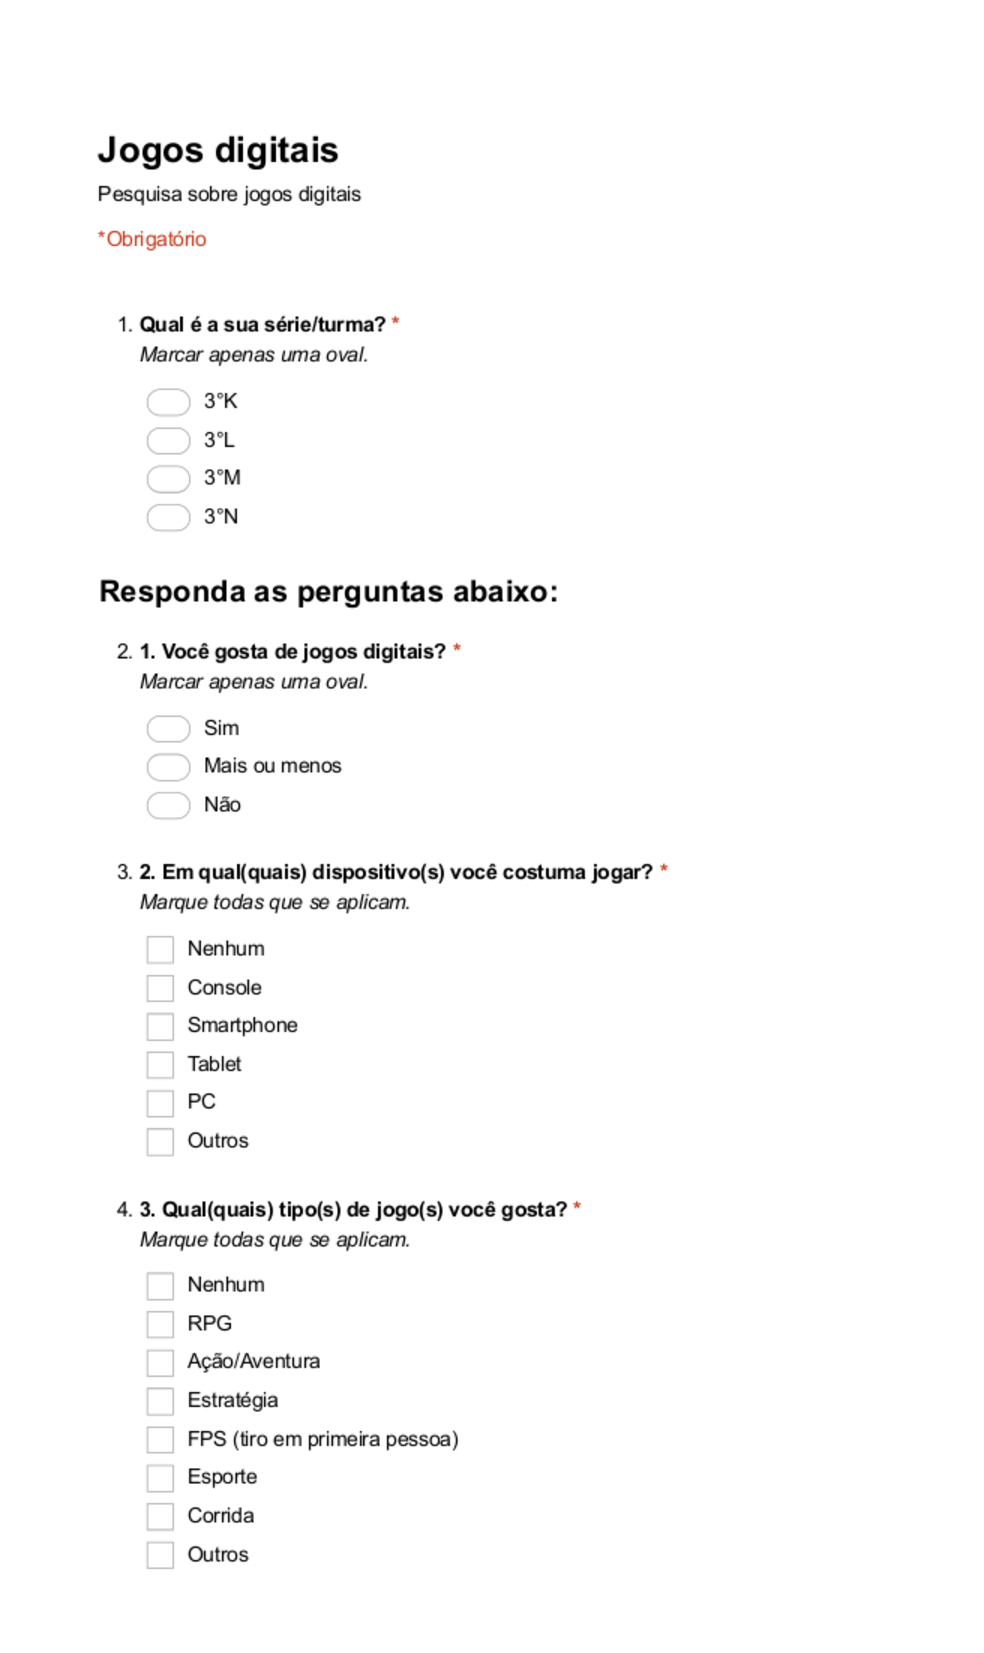
\includegraphics[width=0.69 \textwidth]{ApeB/Img_pesq_ini/pi_part1}
	\caption{Pesquisa inicial: parte 1}
	\label{appb_fig:pi_part1}
\end{figura}

\newpage

\begin{figura}[ht]
	\centering
	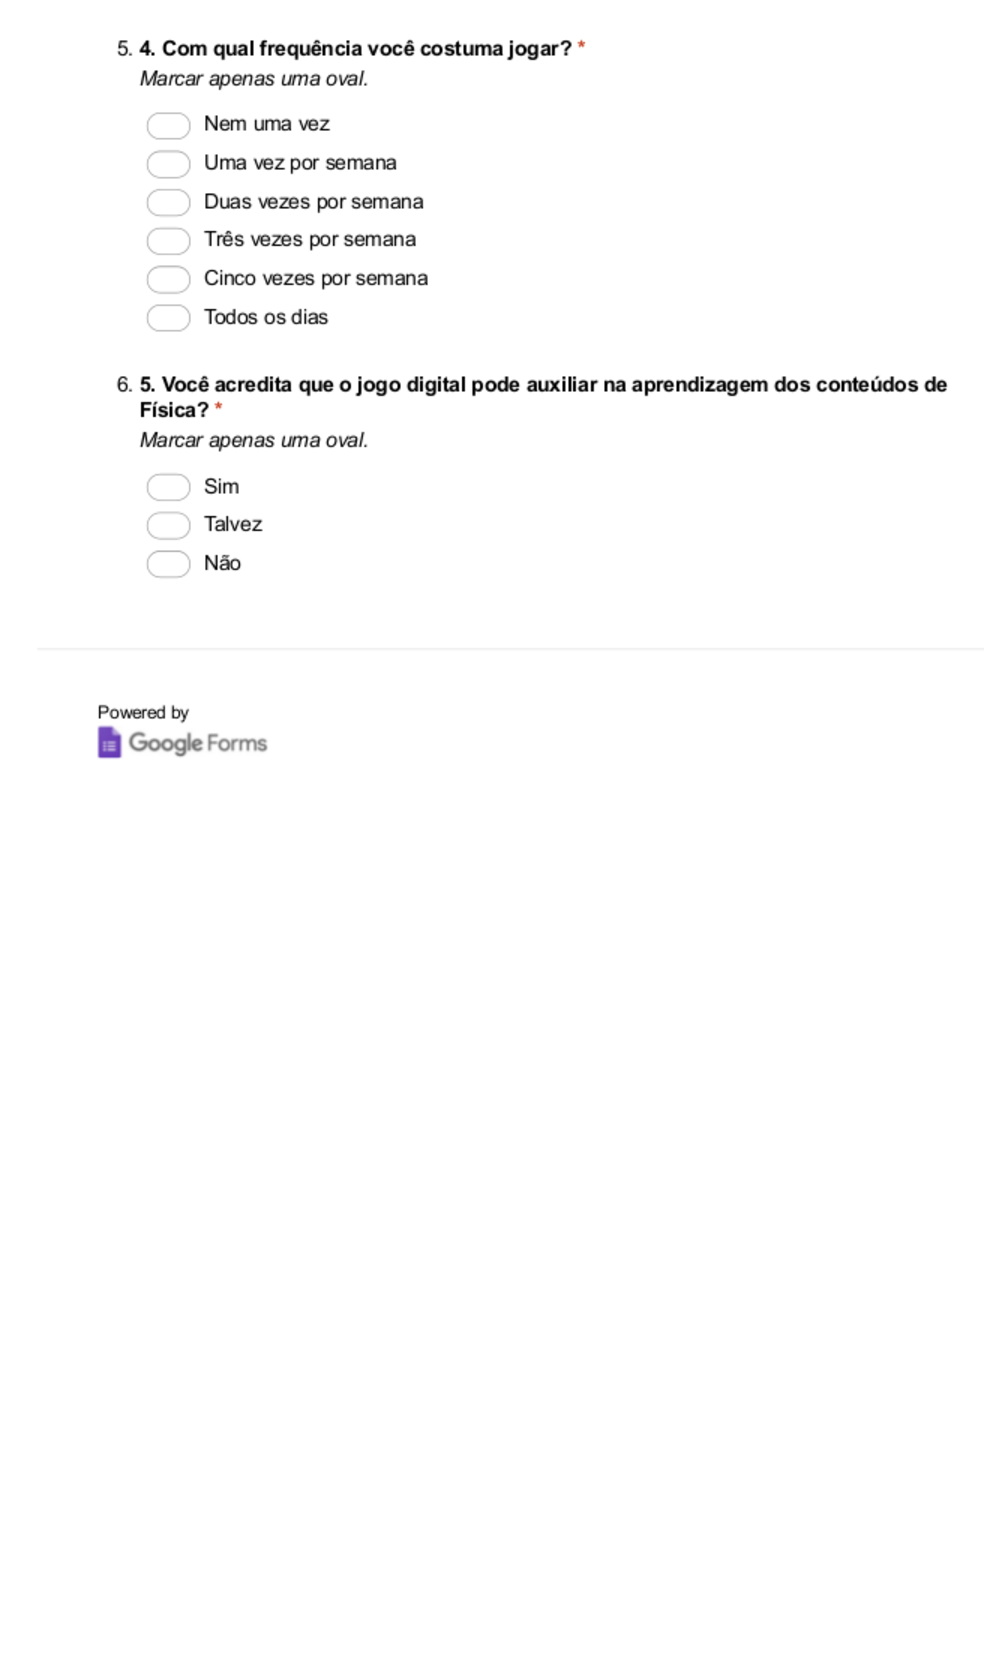
\includegraphics[width=0.69 \textwidth]{ApeB/Img_pesq_ini/pi_part2}
	\caption{Pesquisa inicial: parte 2}
	\label{appb_fig:pi_part2}
\end{figura}

\newpage

\section{Resultados da Pesquisa Inicial}\label{app_b:res_inicial}

\begin{grafico}[ht]
	\centering
	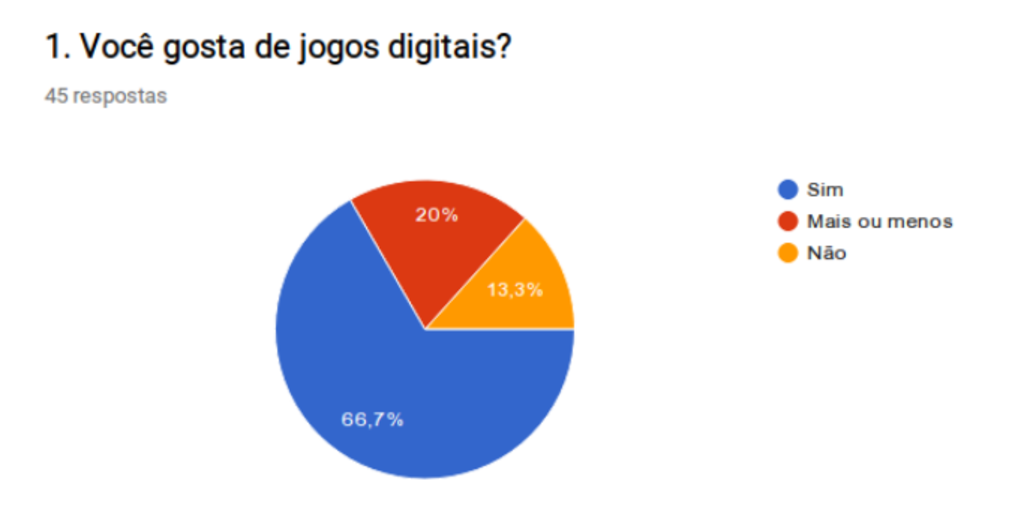
\includegraphics[width=0.9 \textwidth]{Resultados_e_Discussoes/Img_pesq_ini/resp_pesq_ini_02}
	\caption{Resultado da Pesquisa Inicial - Pergunta 1}
	\label{appb_fig:pi_res_perg1}
\end{grafico}

\begin{grafico}[ht]
	\centering
	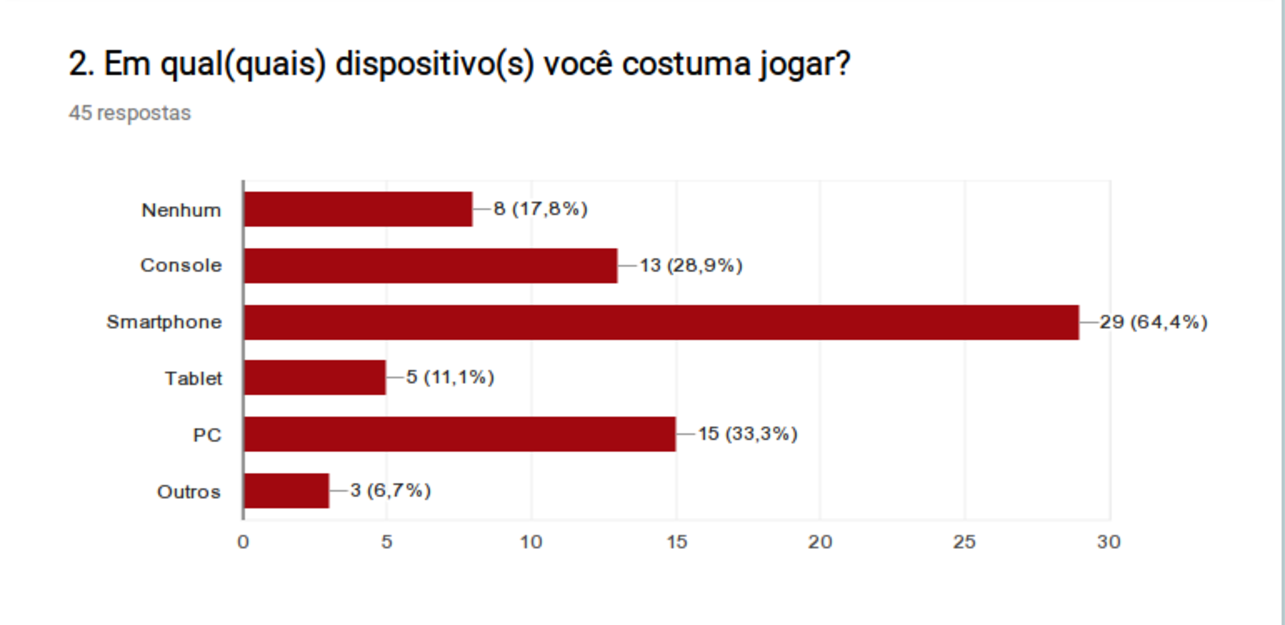
\includegraphics[width=1.0 \textwidth]{Resultados_e_Discussoes/Img_pesq_ini/resp_pesq_ini_03}
	\caption{Resultado da Pesquisa Inicial - Pergunta 2}
	\label{appb_fig:pi_res_perg2}
\end{grafico}

\newpage

\begin{grafico}[ht]
	\centering
	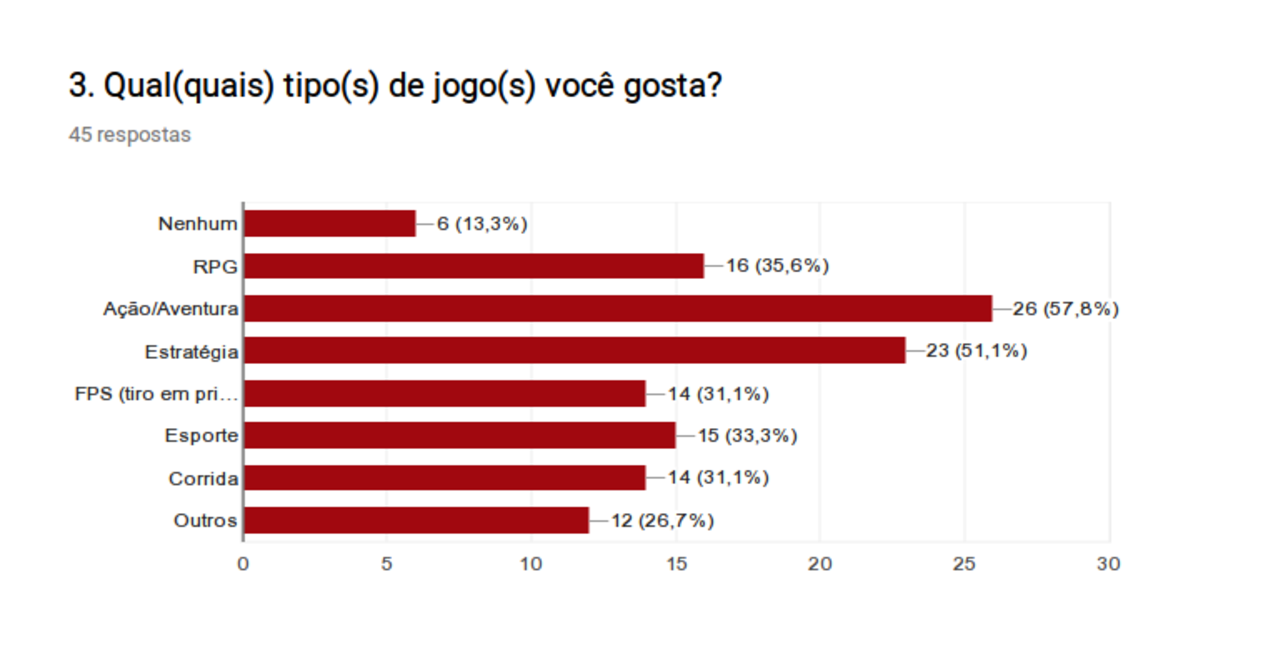
\includegraphics[width=1.0 \textwidth]{Resultados_e_Discussoes/Img_pesq_ini/resp_pesq_ini_04}
	\caption{Resultado da Pesquisa Inicial - Pergunta 3}
	\label{appb_fig:pi_res_perg3}
\end{grafico}

\begin{grafico}[ht]
	\centering
	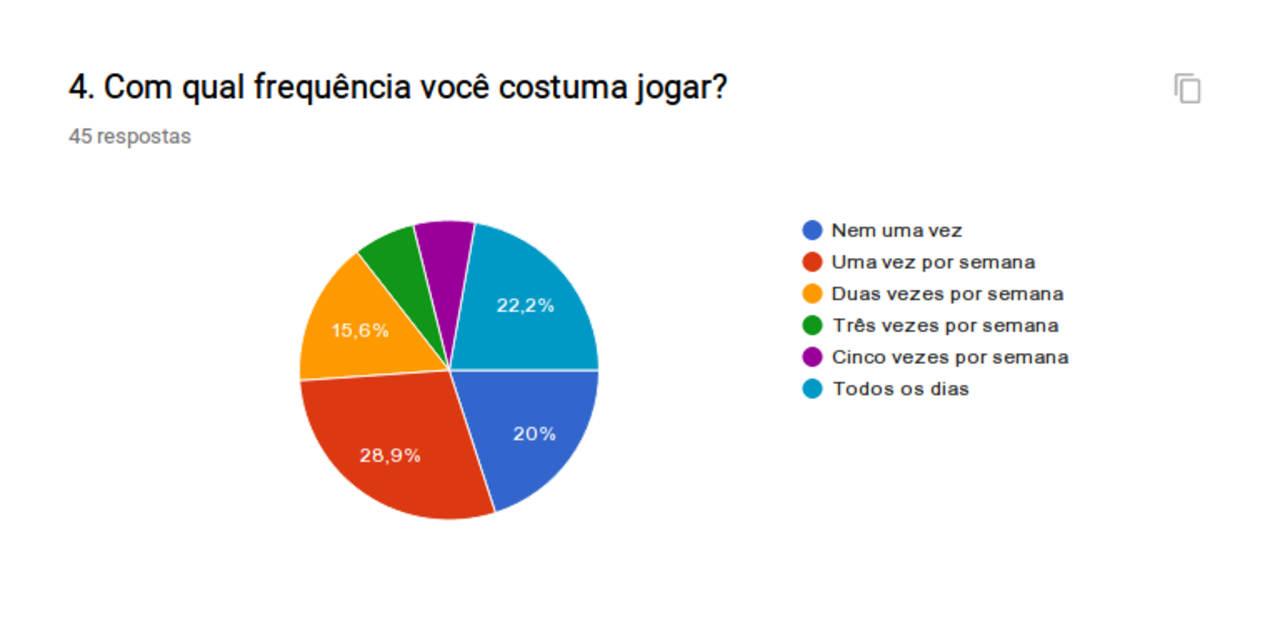
\includegraphics[width=1.0 \textwidth]{Resultados_e_Discussoes/Img_pesq_ini/resp_pesq_ini_05}
	\caption{Resultado da Pesquisa Inicial - Pergunta 4}
	\label{appb_fig:pi_res_perg4}
\end{grafico}

\newpage

\begin{grafico}[ht]
	\centering
	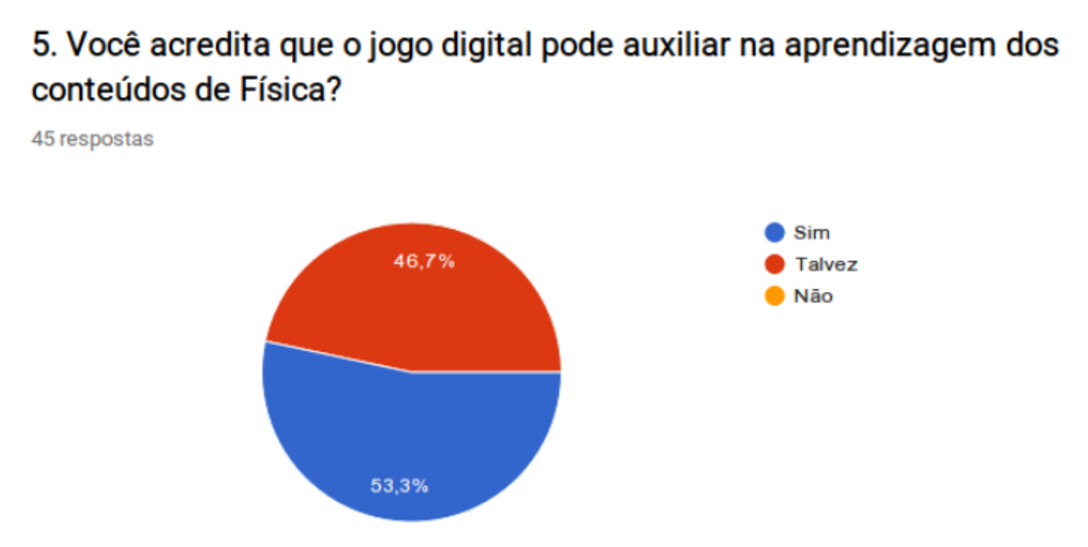
\includegraphics[width=0.9 \textwidth]{Resultados_e_Discussoes/Img_pesq_ini/resp_pesq_ini_06}
	\caption{Resultado da Pesquisa Inicial - Pergunta 5}
	\label{appb_fig:pi_res_perg5}
\end{grafico}

\newpage

\section{Testes}\label{app_b:teste}

\begin{figura}[h]
	\centering
	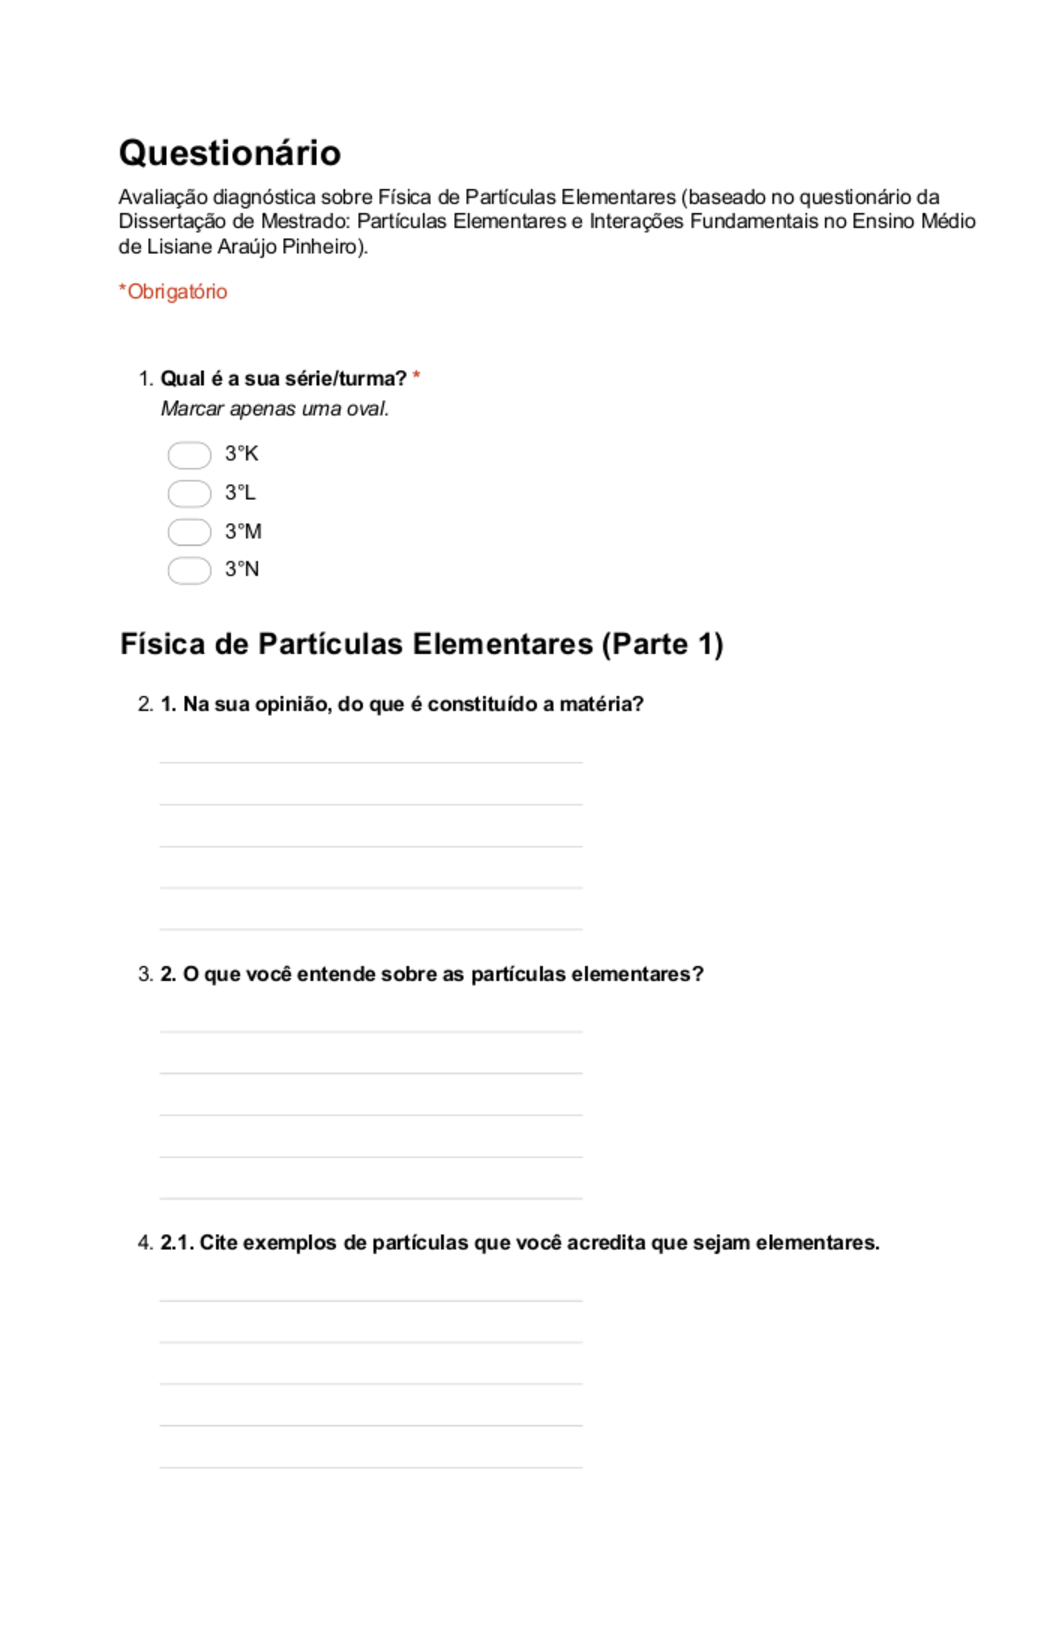
\includegraphics[width=0.70 \textwidth]{ApeB/Img_test/teste_part1}
	\caption{Teste: parte 1}
	\label{appb_fig:test_part1}
\end{figura}

\newpage

\begin{figura}[ht]
	\centering
	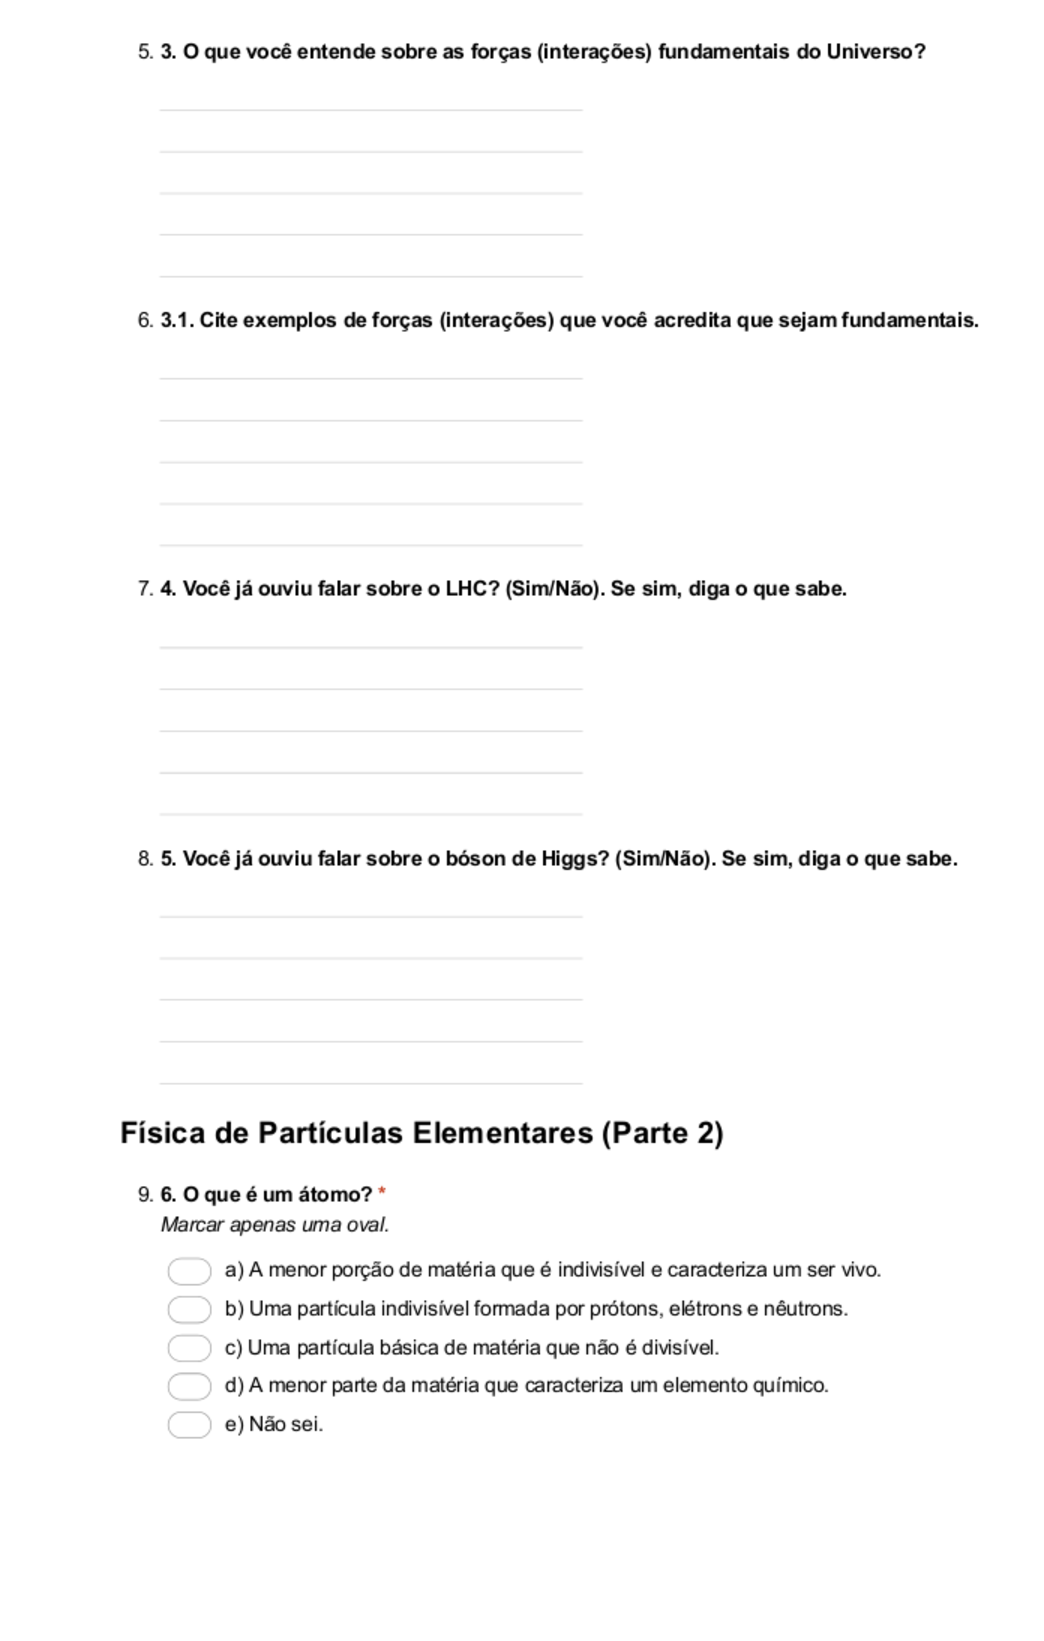
\includegraphics[width=0.70 \textwidth]{ApeB/Img_test/teste_part2}
	\caption{Teste: parte 2}
	\label{appb_fig:test_part2}
\end{figura}

\newpage

\begin{figura}[ht]
	\centering
	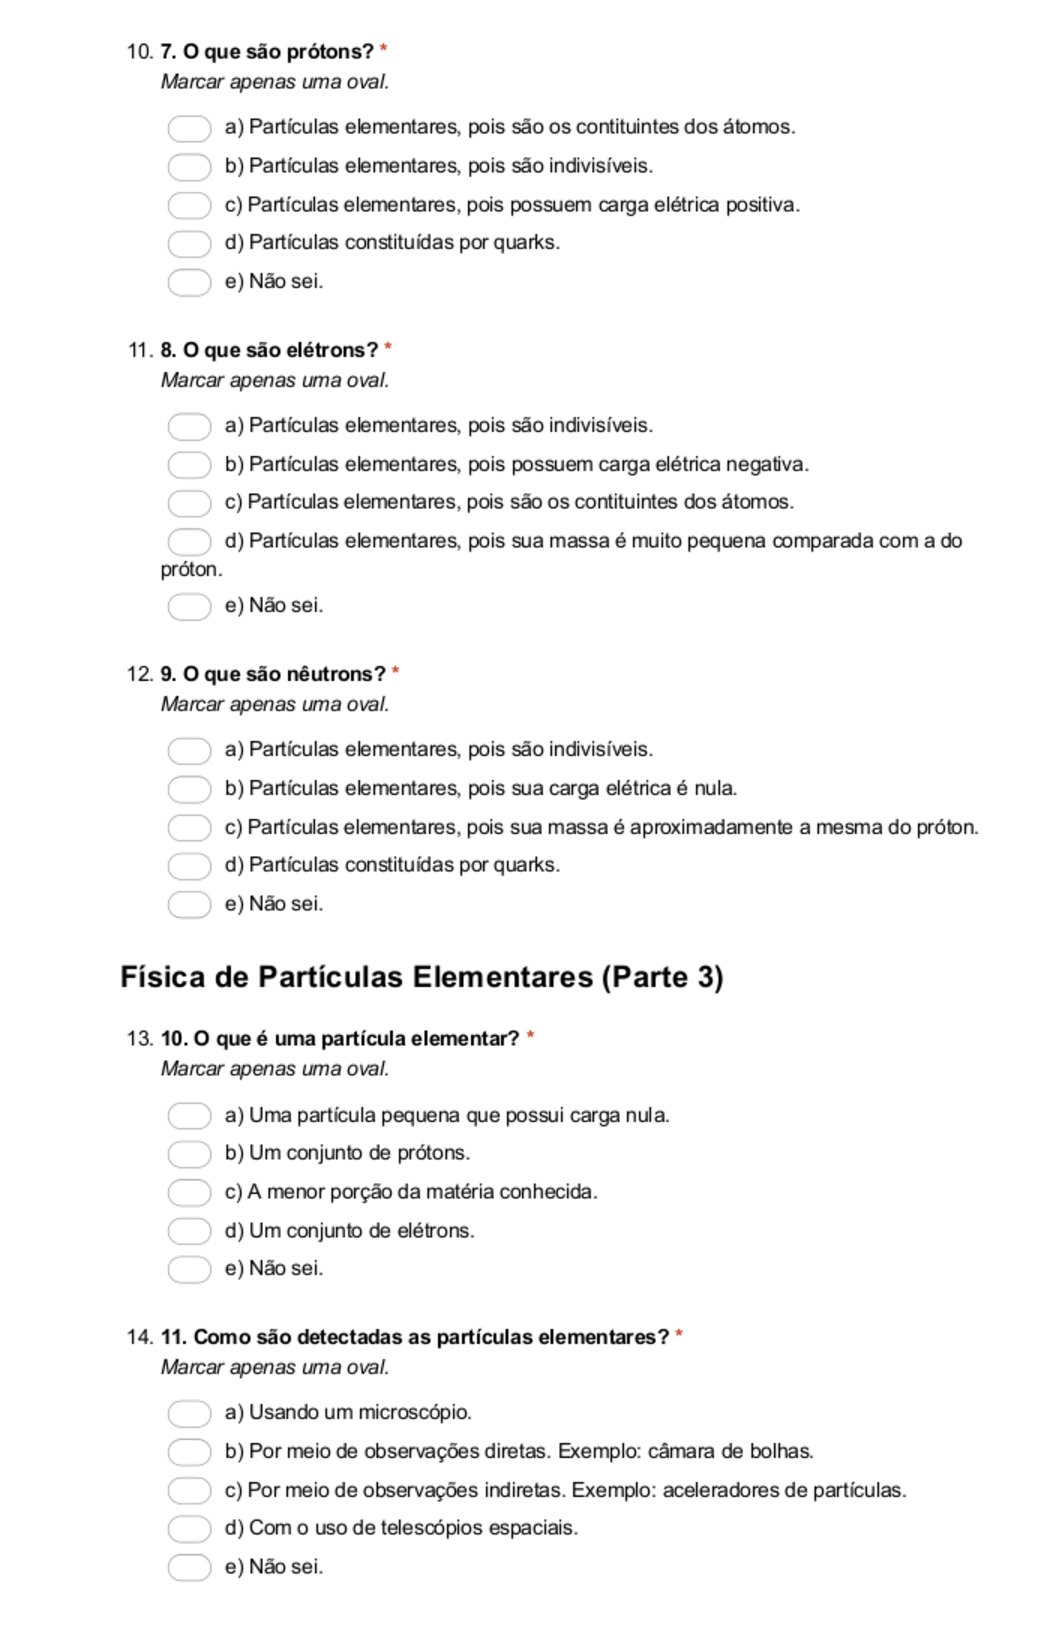
\includegraphics[width=0.70 \textwidth]{ApeB/Img_test/teste_part3}
	\caption{Teste: parte 3}
	\label{appb_fig:test_part3}
\end{figura}

\newpage

\begin{figura}[ht]
	\centering
	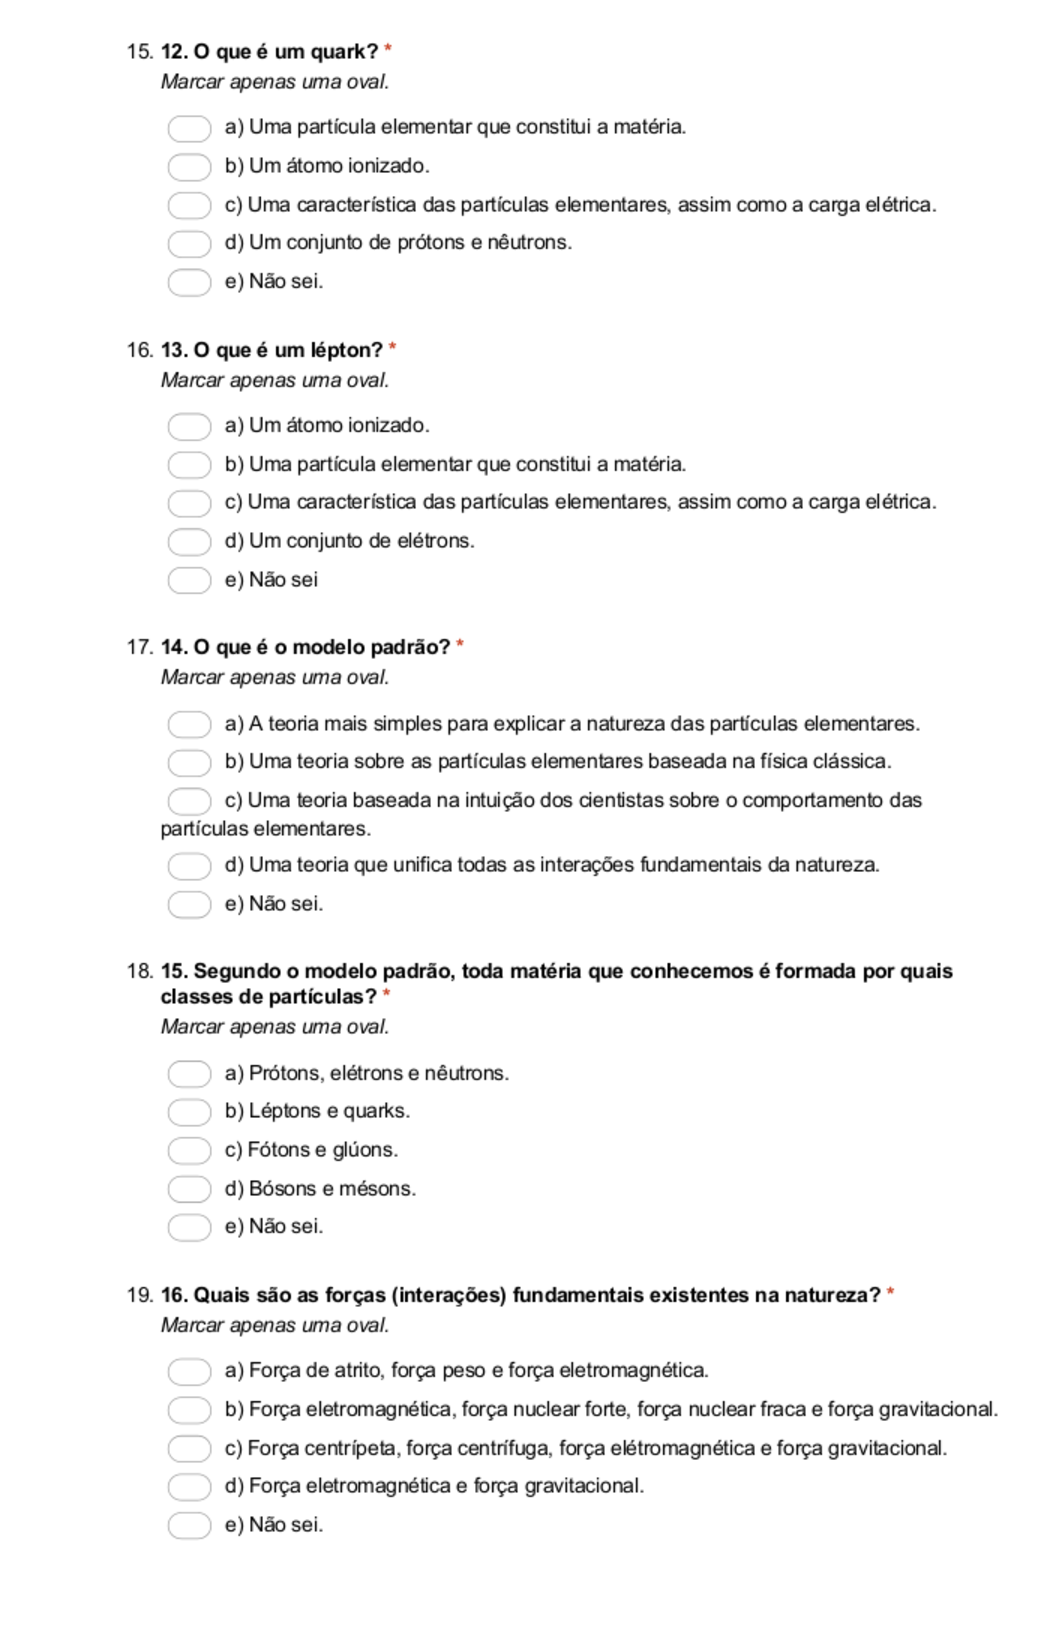
\includegraphics[width=0.70 \textwidth]{ApeB/Img_test/teste_part4}
	\caption{Teste: parte 4}
	\label{appb_fig:test_part4}
\end{figura}

\newpage

\begin{figura}[ht]
	\centering
	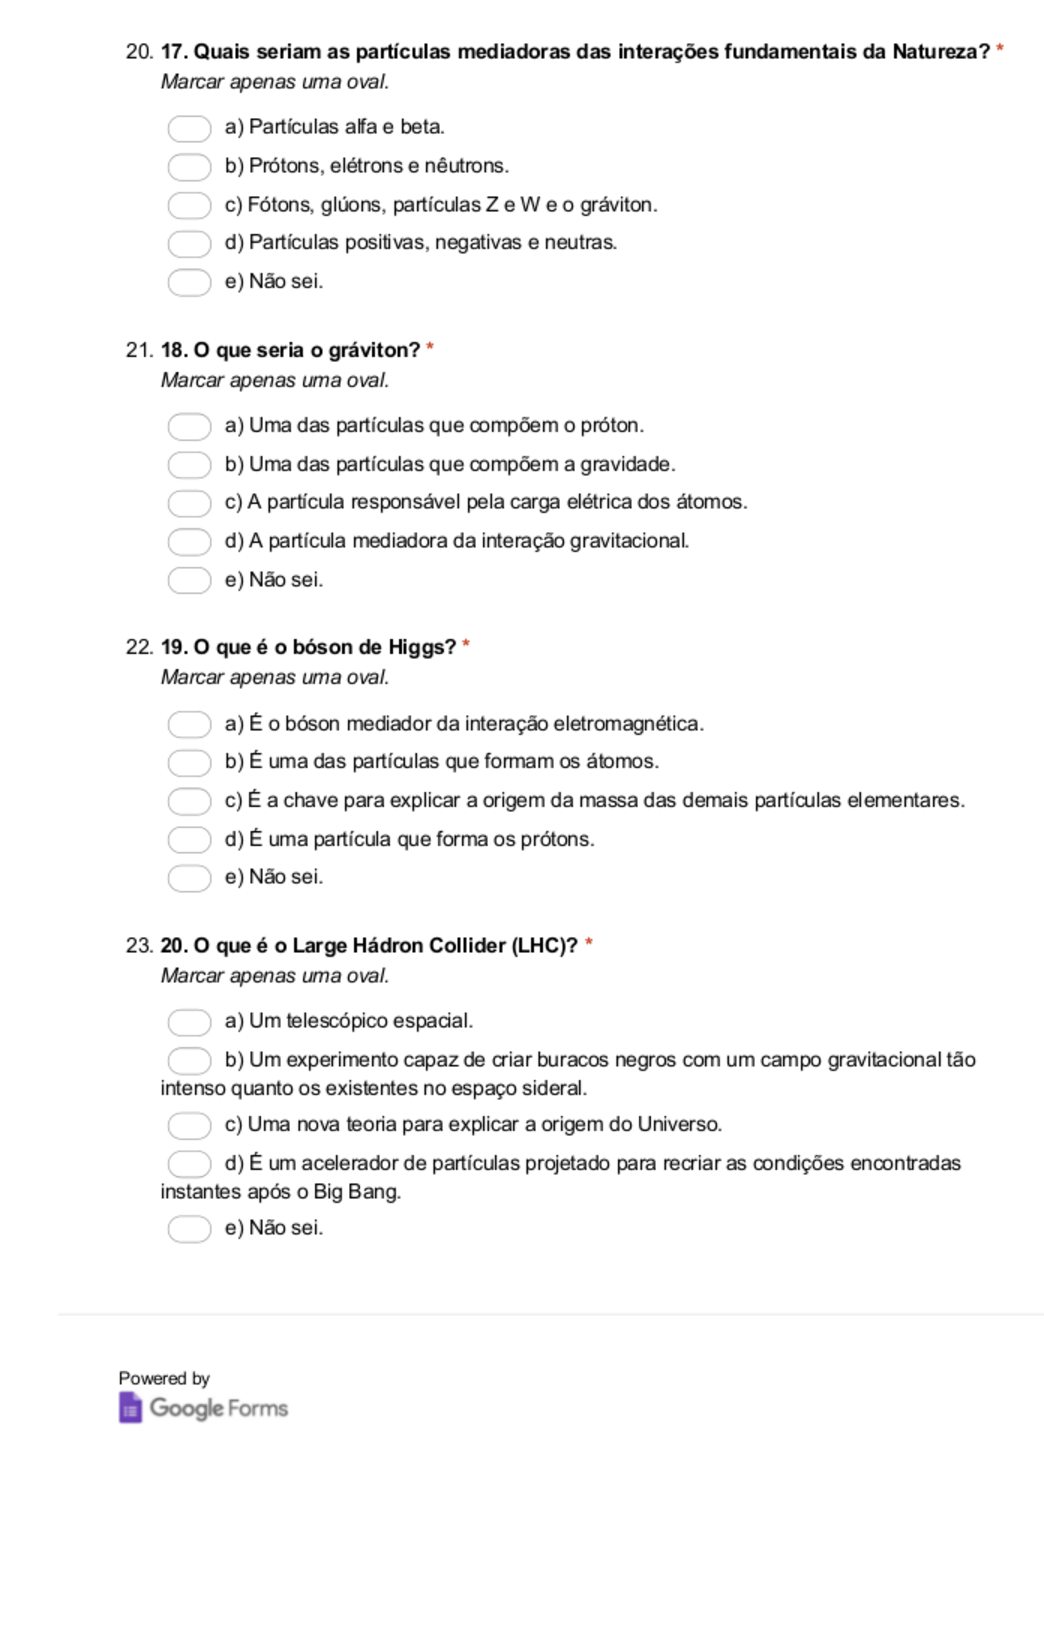
\includegraphics[width=0.70 \textwidth]{ApeB/Img_test/teste_part5}
	\caption{Teste: parte 5}
	\label{appb_fig:test_part5}
\end{figura}

\newpage

\section{Resultados dos Testes}\label{app_b:res_teste}

\begin{tabela}[ht]
	\centering
	\caption{Resultado dos Testes - Pergunta 1}
	\label{my-label}
	\begin{tabular}{@{}lcc@{}}
		\toprule
		& Pr�-Teste (\%) & P�s-Teste (\%) \\ \midrule
		�tomos                       & 21,2           & 42,5           \\
		Pr�tons, el�trons e n�utrons & 3,0            & 4,3            \\
		Part�culas elementares       & 0,0            & 21,3           \\
		Outras respostas             & 36,4           & 12,8           \\
		Respostas em branco          & 39,4           & 19,1           \\ \bottomrule
	\end{tabular}
\end{tabela}

\begin{tabela}[ht]
	\centering
	\caption{Resultado dos Testes - Pergunta 2}
	\label{my-label}
	\begin{tabular}{@{}lcc@{}}
		\toprule
		& Pr�-Teste (\%) & P�s-Teste (\%) \\ \midrule
		�tomos                       & 3,0            & 8,5            \\
		Pr�tons, el�trons e n�utrons & 9,1            & 8,5            \\
		Part�culas sem subestruturas & 18,2           & 46,8           \\
		Outras respostas             & 24,2           & 8,5            \\
		Branco                       & 45,5           & 27,7           \\ \bottomrule
	\end{tabular}
\end{tabela}

\begin{tabela}[ht]
	\centering
	\caption{Resultado dos Testes - Pergunta 3}
	\label{my-label}
	\begin{tabular}{@{}lcc@{}}
		\toprule
		& Pr�-Teste (\%) & P�s-Teste (\%) \\ \midrule
		Citou as 4 intera��es          & 9,1            & 36,2           \\
		Citou 2 intera��es             & 12,1           & 8,5            \\
		Citou pelo menos uma intera��o & 3,0            & 2,1            \\
		Outras respostas               & 9,1            & 40,4           \\
		Resposta em branco             & 66,7           & 12,8           \\ \bottomrule
	\end{tabular}
\end{tabela}

\newpage

\begin{tabela}[ht]
	\centering
	\caption{Resultado dos Testes - Pergunta 4}
	\label{my-label}
	\begin{tabular}{@{}lcc@{}}
		\toprule
		& Pr�-Teste (\%) & P�s-Teste (\%) \\ \midrule
		N�o                         & 54,5           & 12,8           \\
		Sim                         & 0,0            & 14,9           \\
		Sim com resposta adequada   & 6,1            & 42,5           \\
		Sim com resposta inadequada & 0,0            & 6,4            \\
		Resposta em branco          & 39,4           & 23,4           \\ \bottomrule
	\end{tabular}
\end{tabela}

\begin{grafico}[ht]
	\centering
	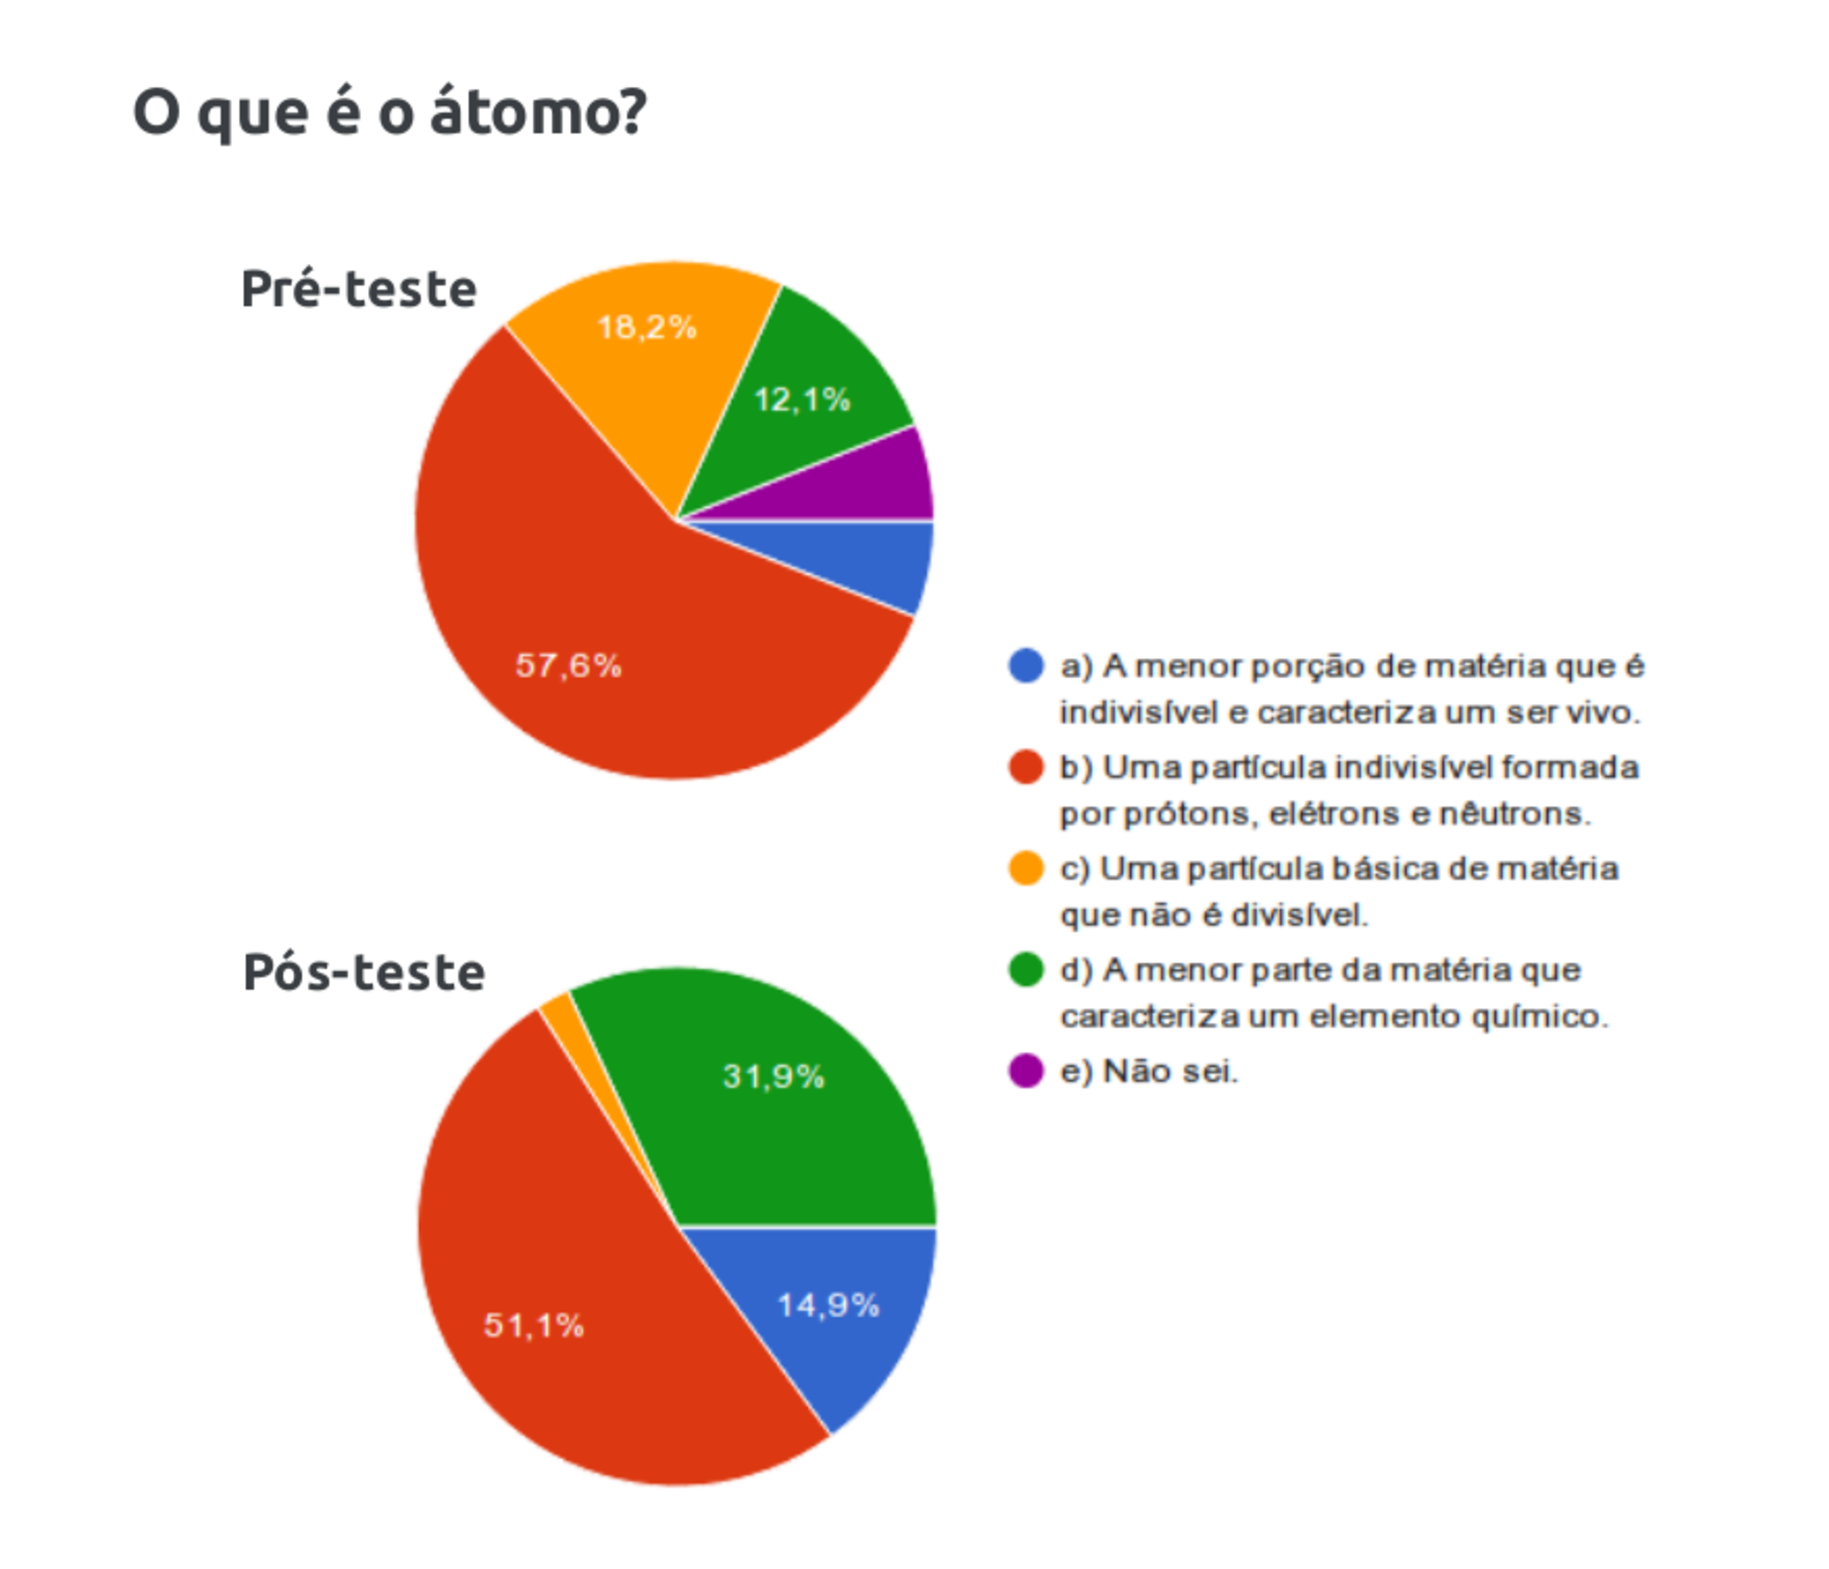
\includegraphics[width=0.61 \textwidth]{Resultados_e_Discussoes/Teste/q5_1}
	\caption{Resultado dos Testes - Pergunta 5}
	\label{appb_fig:test_res_perg5}
\end{grafico}

\begin{grafico}[ht]
	\centering
	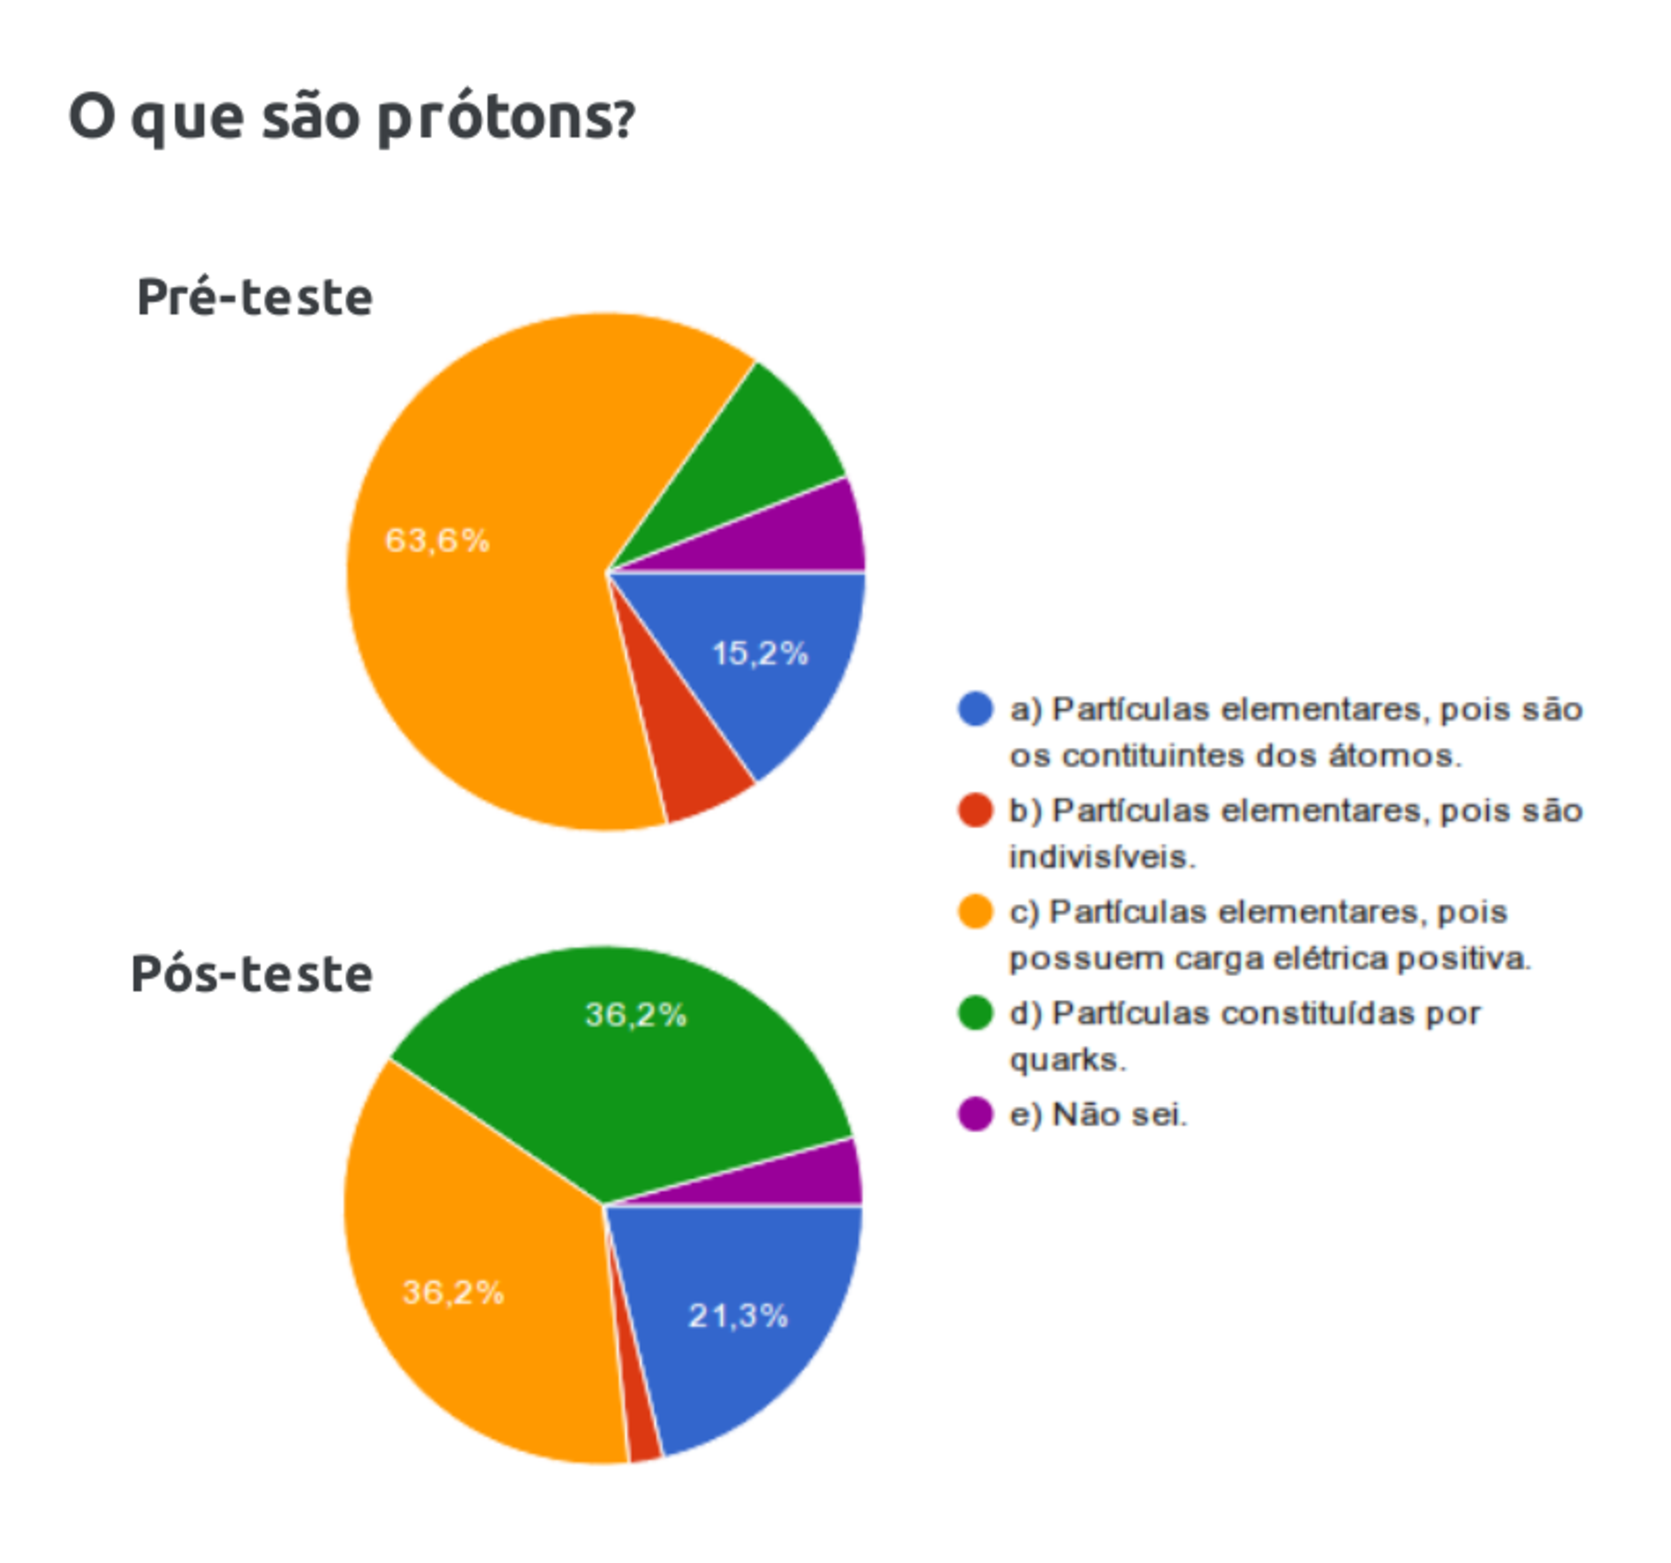
\includegraphics[width=0.56 \textwidth]{Resultados_e_Discussoes/Teste/q6_1}
	\caption{Resultado dos Testes - Pergunta 6}
	\label{appb_fig:test_res_perg6}
\end{grafico}

\newpage

\begin{grafico}[ht]
	\centering
	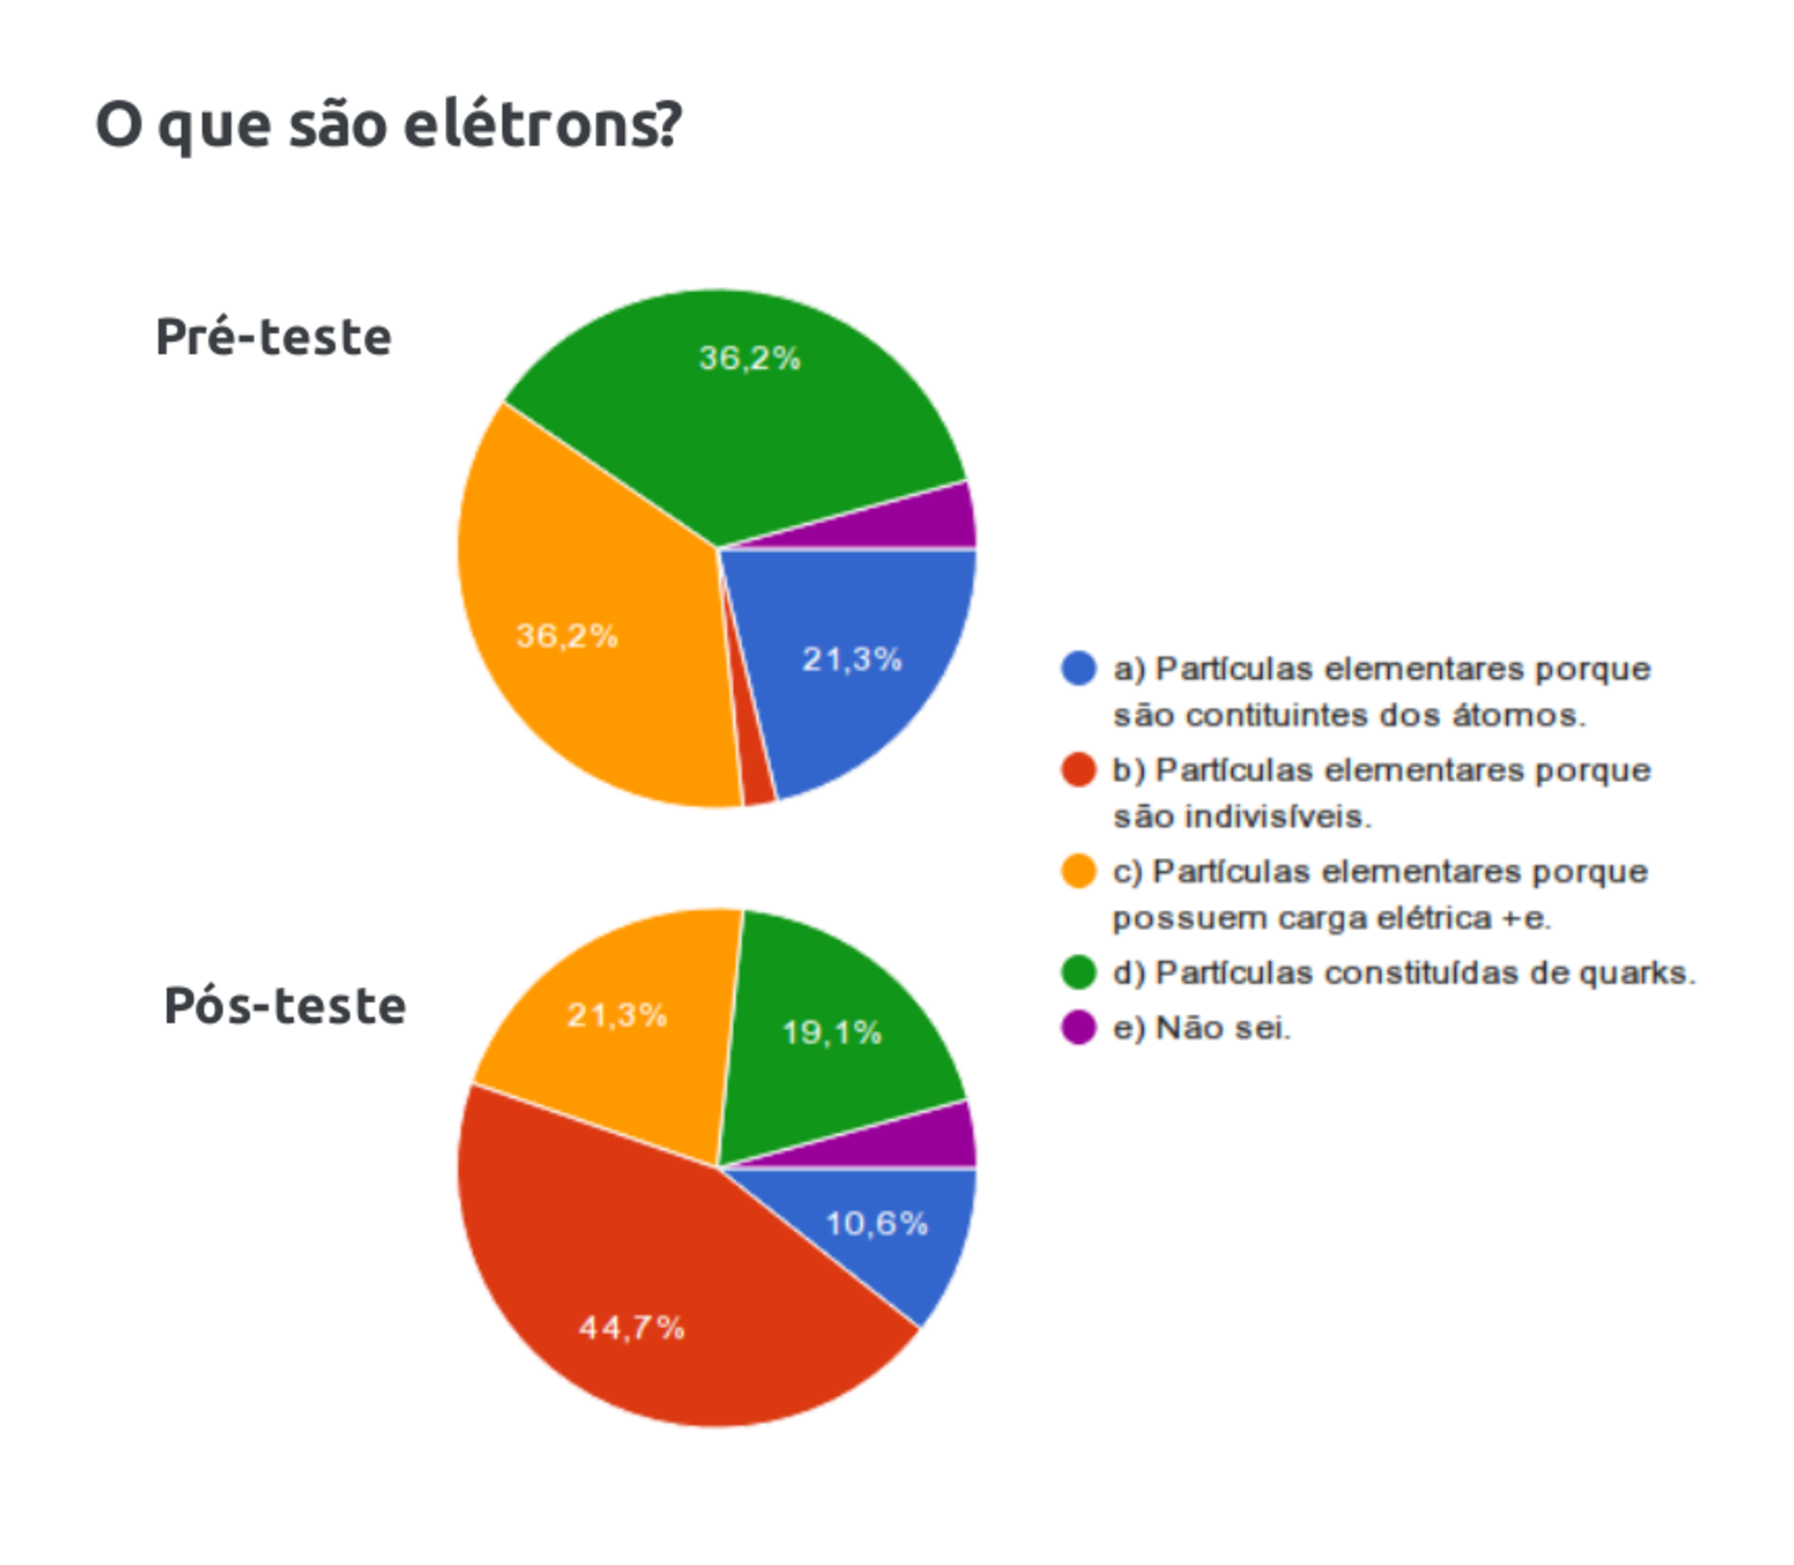
\includegraphics[width=0.62 \textwidth]{Resultados_e_Discussoes/Teste/q7_1}
	\caption{Resultado dos Testes - Pergunta 7}
	\label{appb_fig:test_res_perg7}
\end{grafico}


\begin{grafico}[ht]
	\centering
	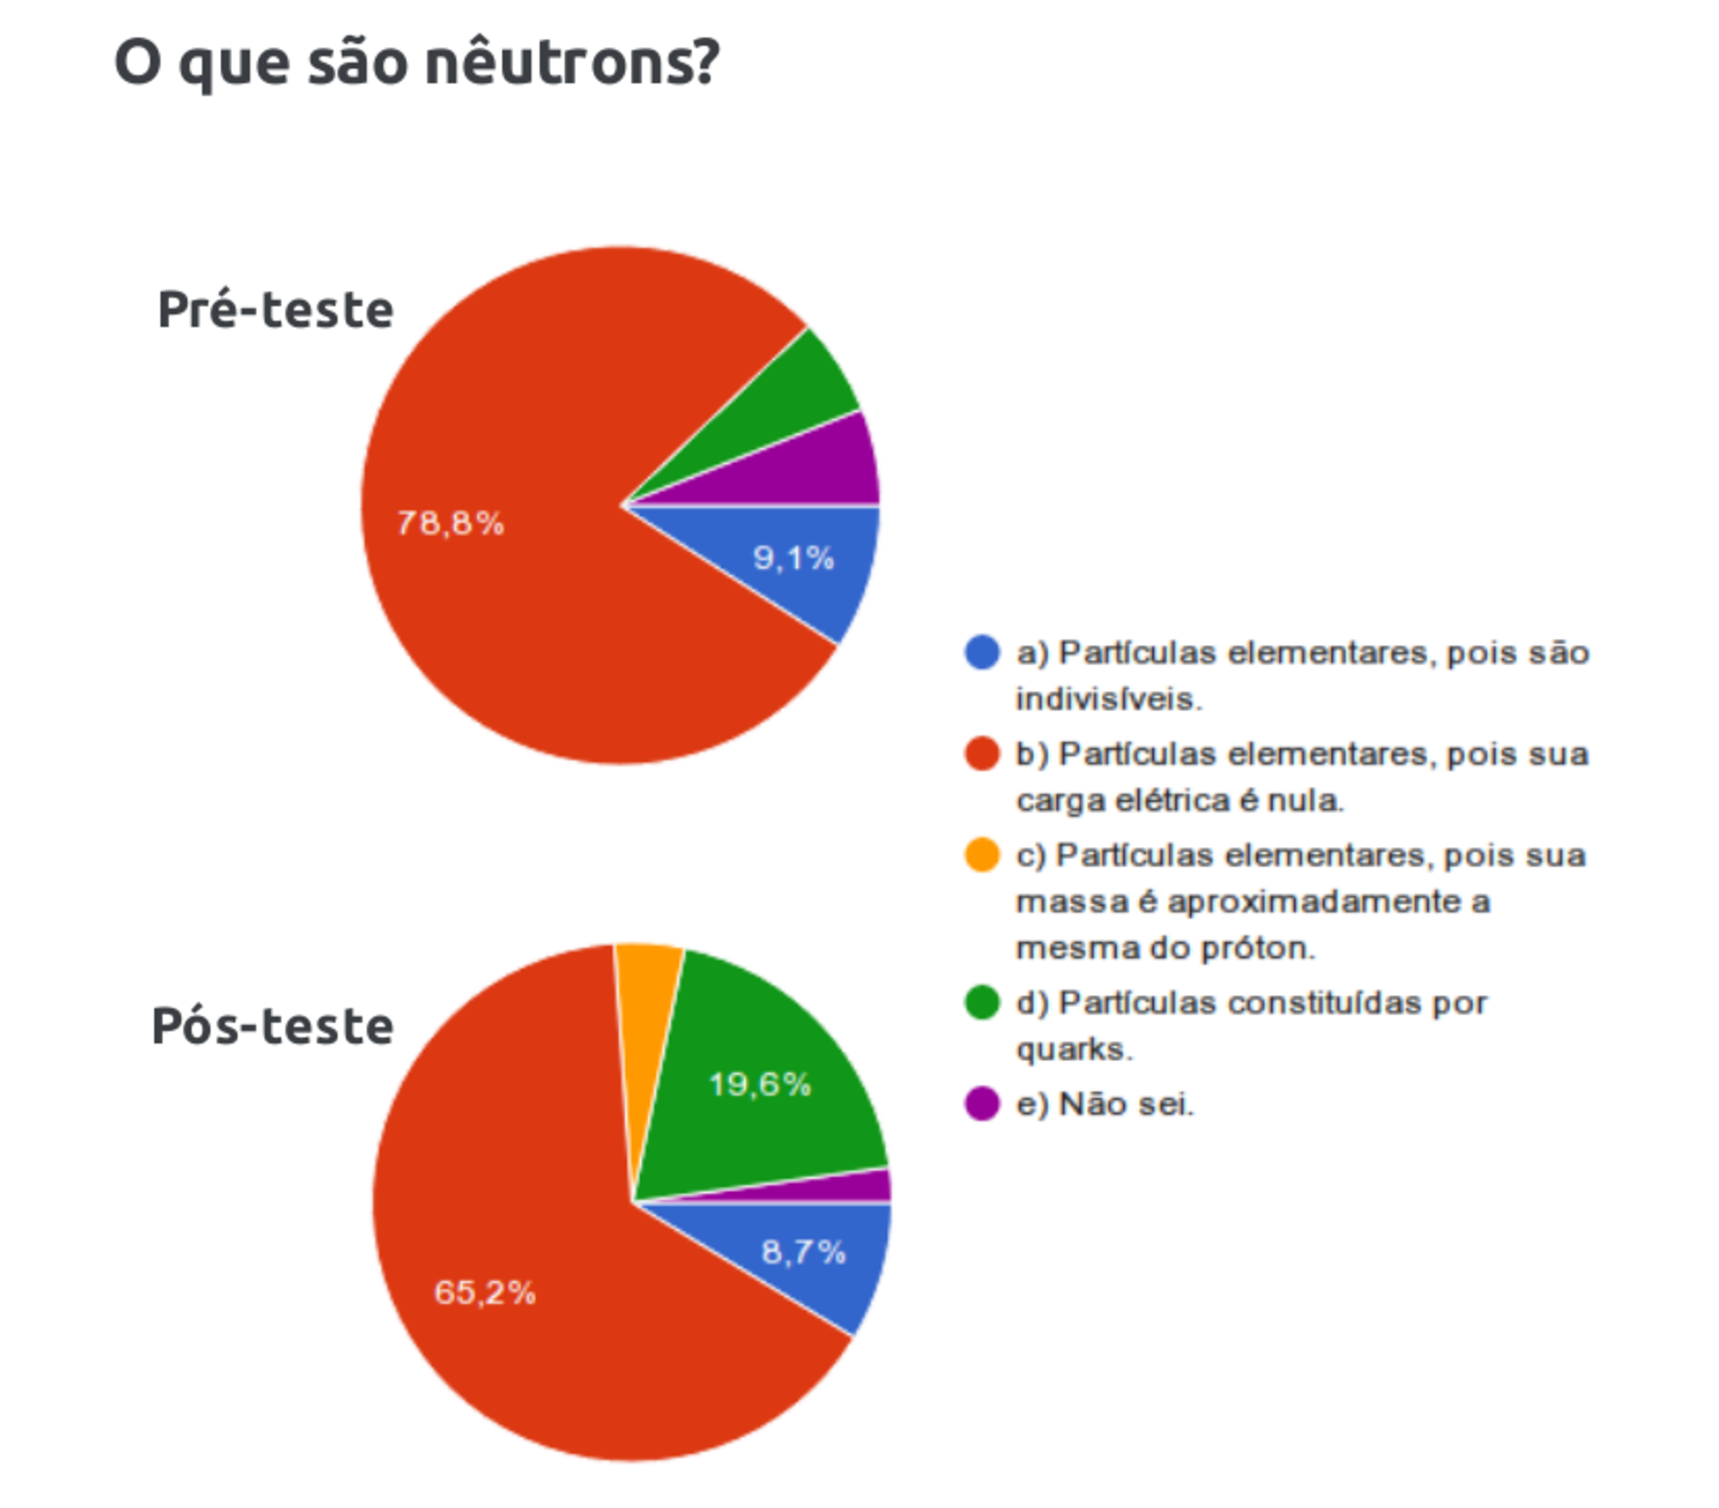
\includegraphics[width=0.57 \textwidth]{Resultados_e_Discussoes/Teste/q8_1}
	\caption{Resultado dos Testes - Pergunta 8}
	\label{appb_fig:test_res_perg8}
\end{grafico}

\newpage

\begin{grafico}[ht]
	\centering
	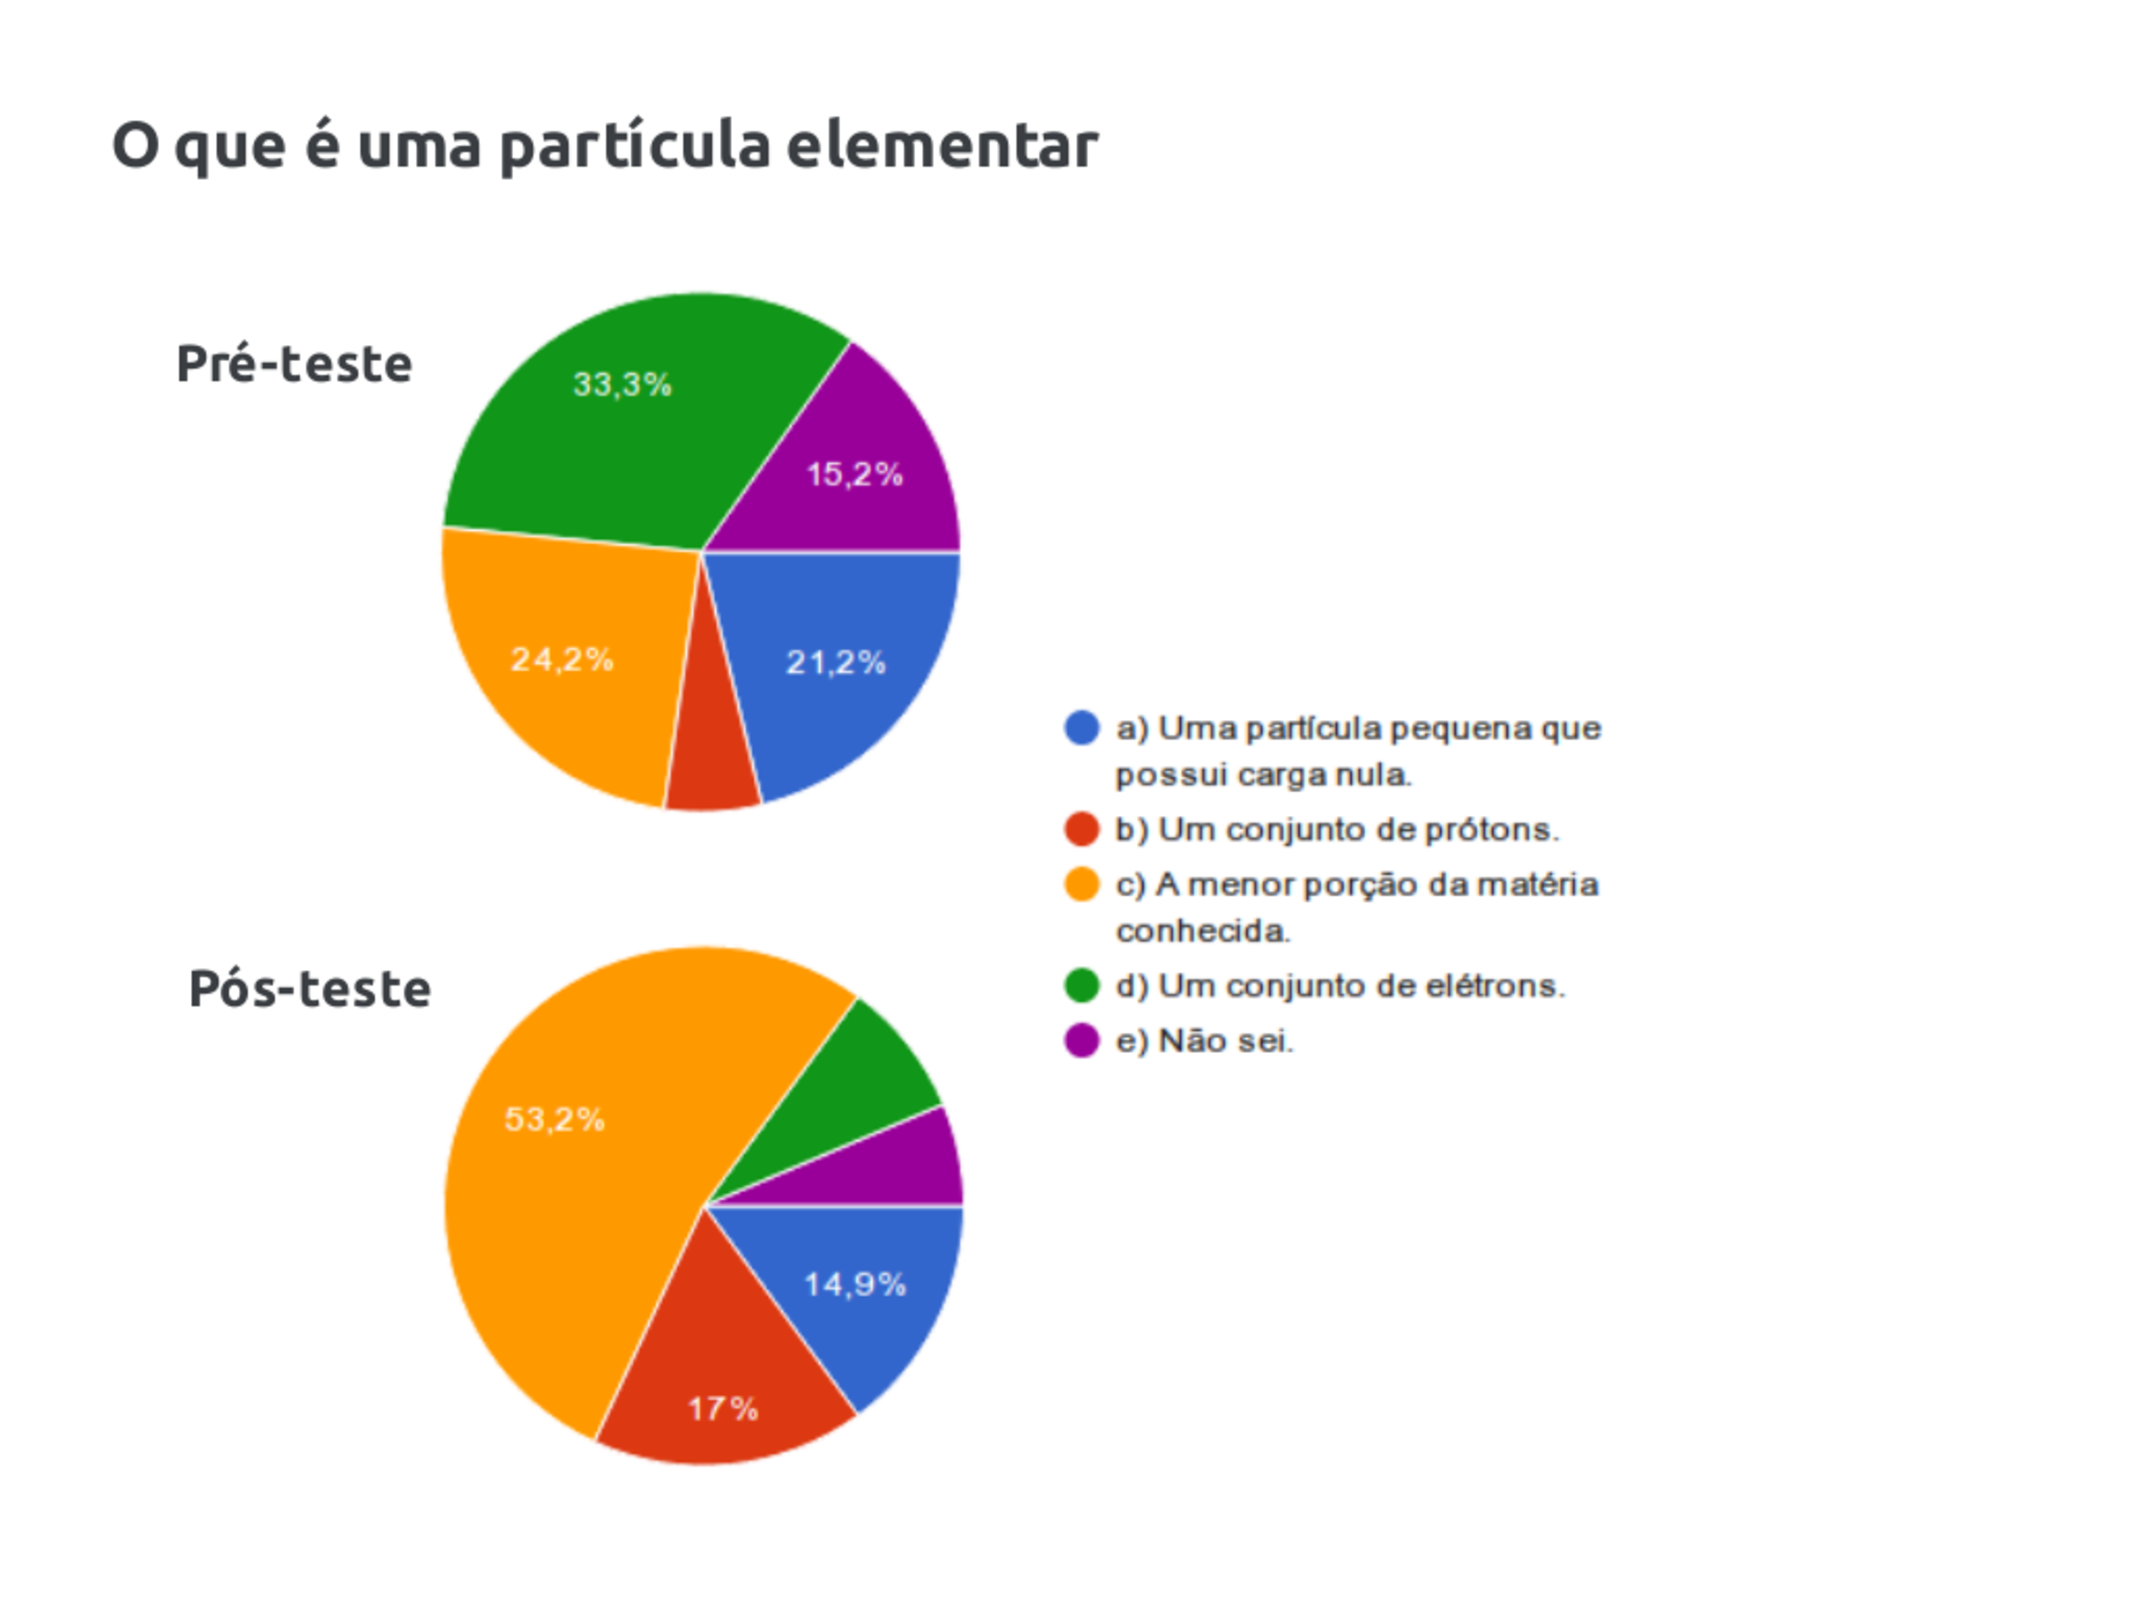
\includegraphics[width=0.71 \textwidth]{Resultados_e_Discussoes/Teste/q10_1}
	\caption{Resultado dos Testes - Pergunta 9}
	\label{appb_fig:test_res_perg9}
\end{grafico}


\begin{grafico}[ht]
	\centering
	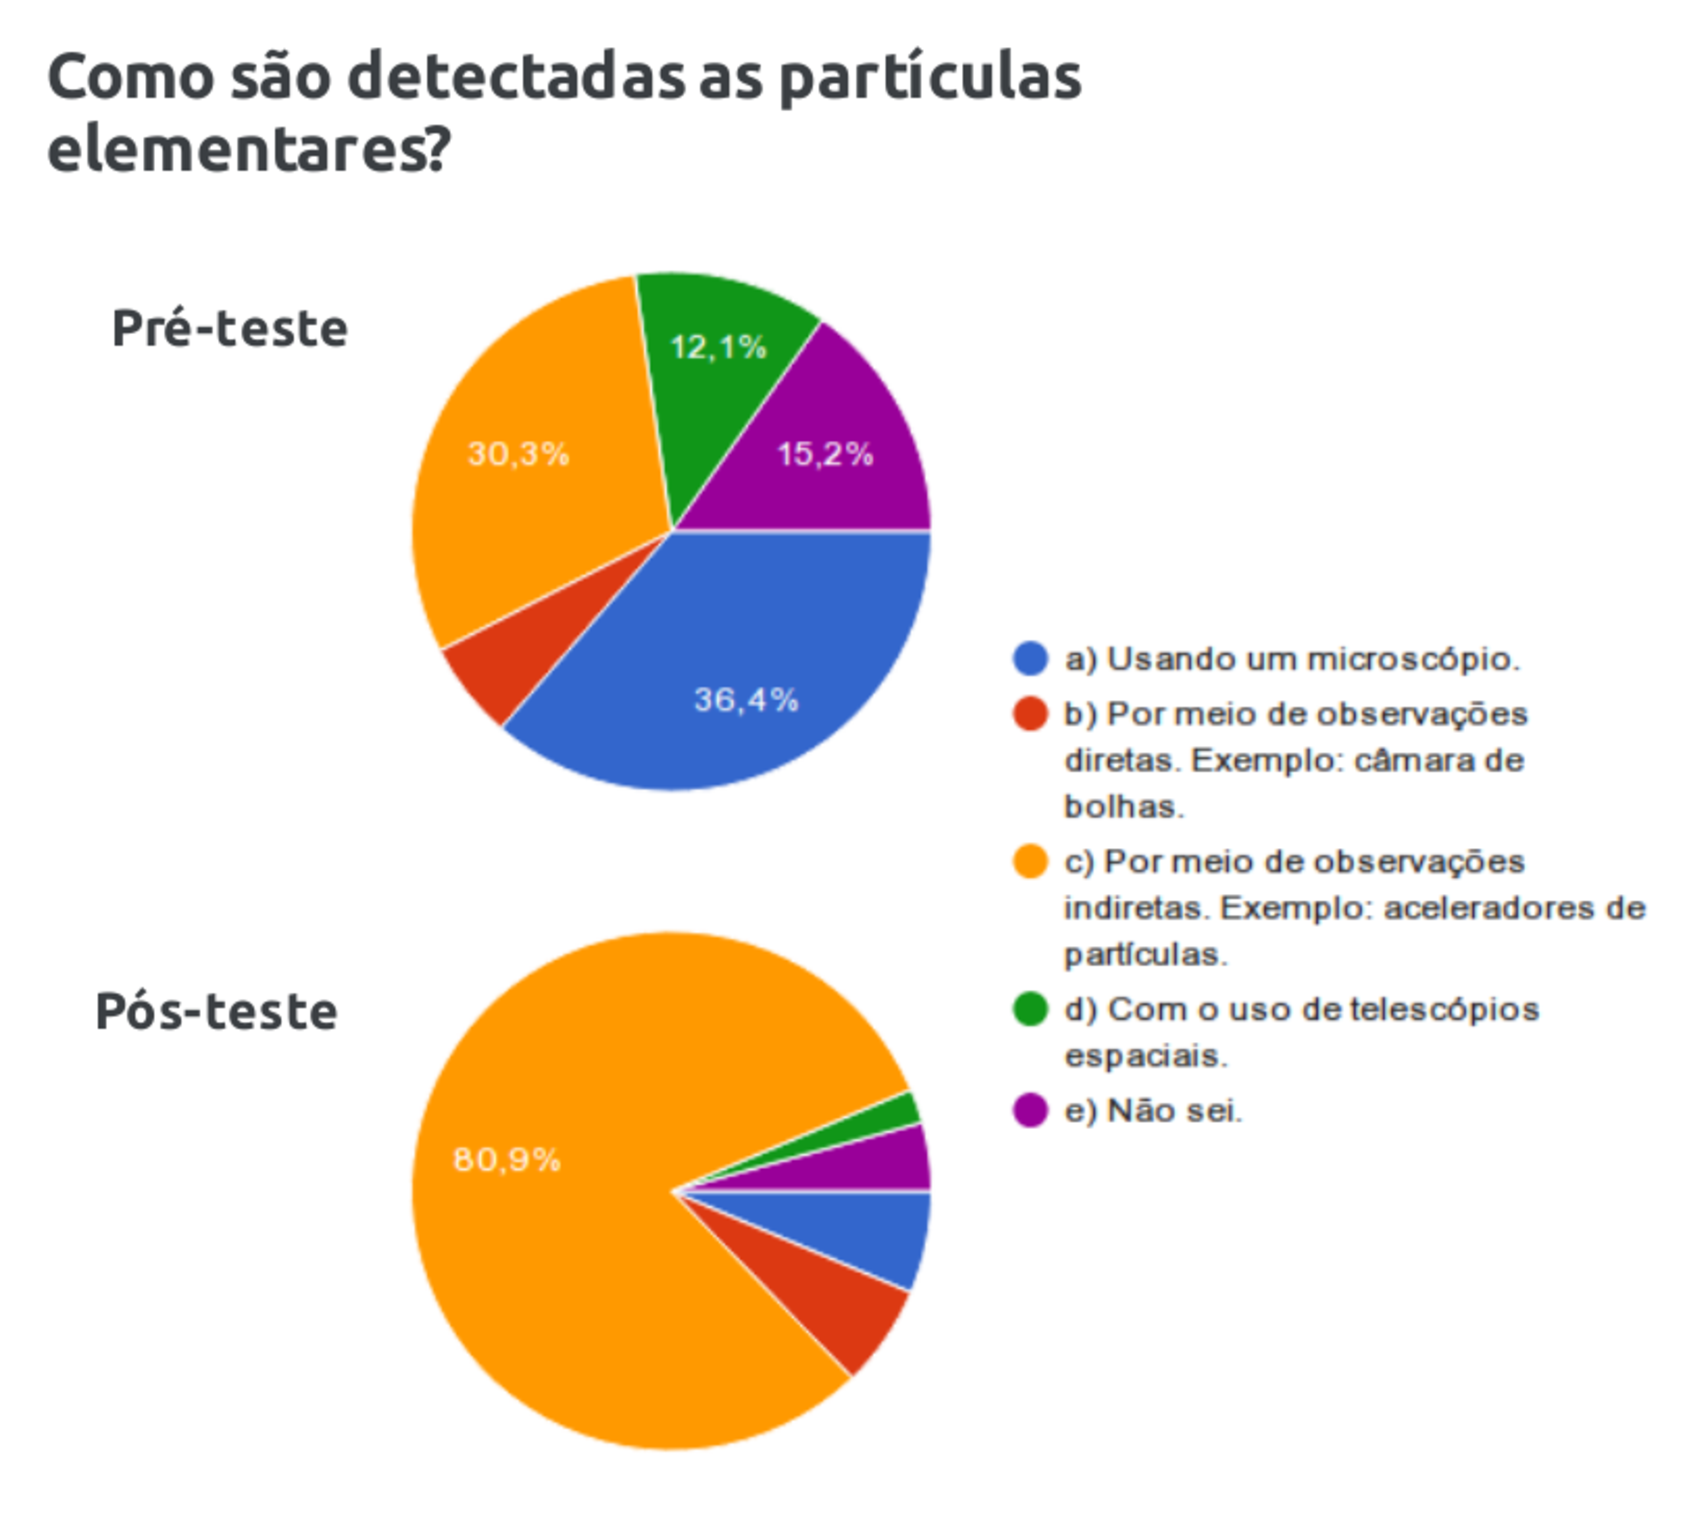
\includegraphics[width=0.57 \textwidth]{Resultados_e_Discussoes/Teste/q11_1}
	\caption{Resultado dos Testes - Pergunta 10}
	\label{appb_fig:test_res_perg10}
\end{grafico}

\newpage

\begin{grafico}[ht]
	\centering
	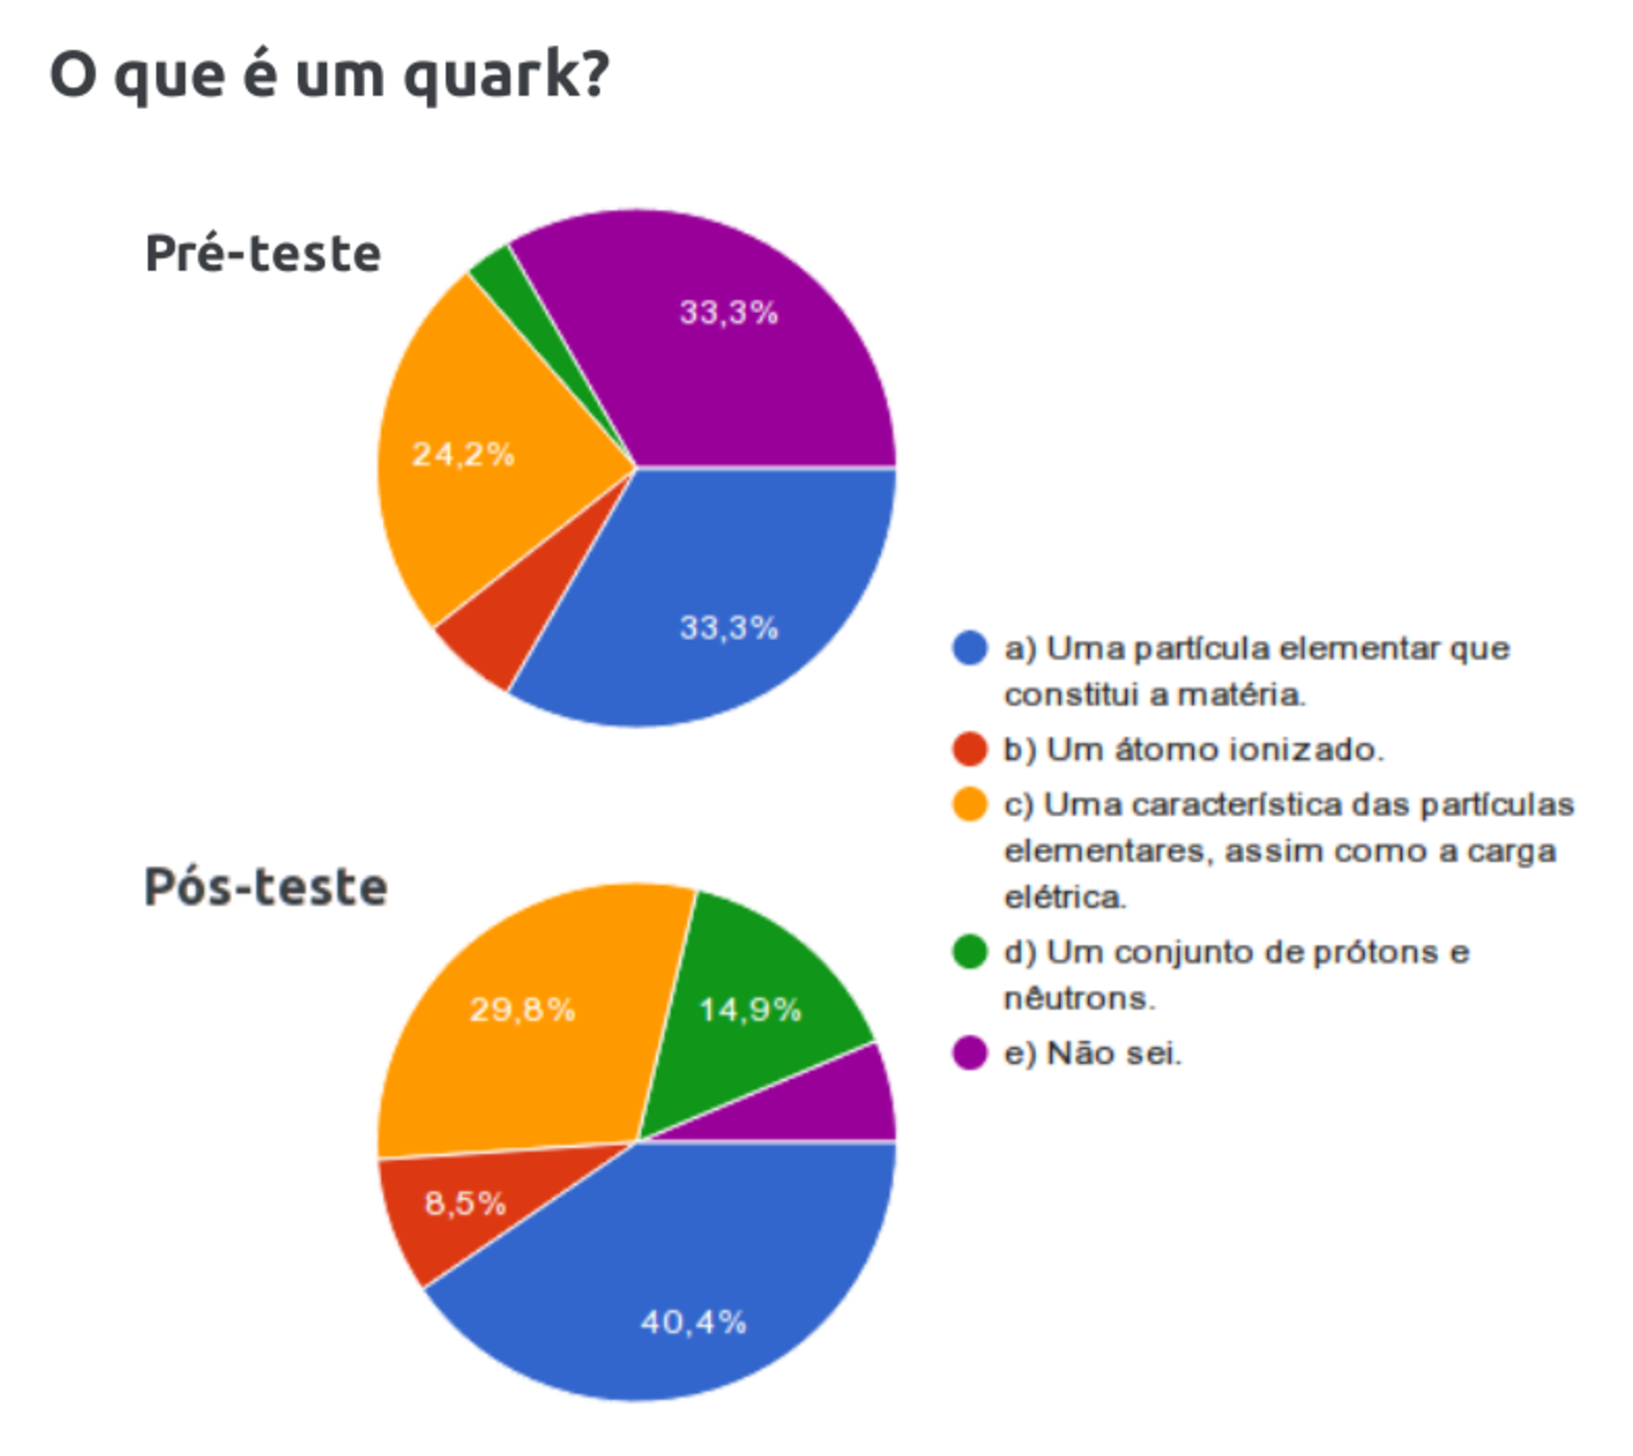
\includegraphics[width=0.57 \textwidth]{Resultados_e_Discussoes/Teste/q12_1}
	\caption{Resultado dos Testes - Pergunta 11}
	\label{appb_fig:test_res_perg11}
\end{grafico}

\begin{grafico}[ht]
	\centering
	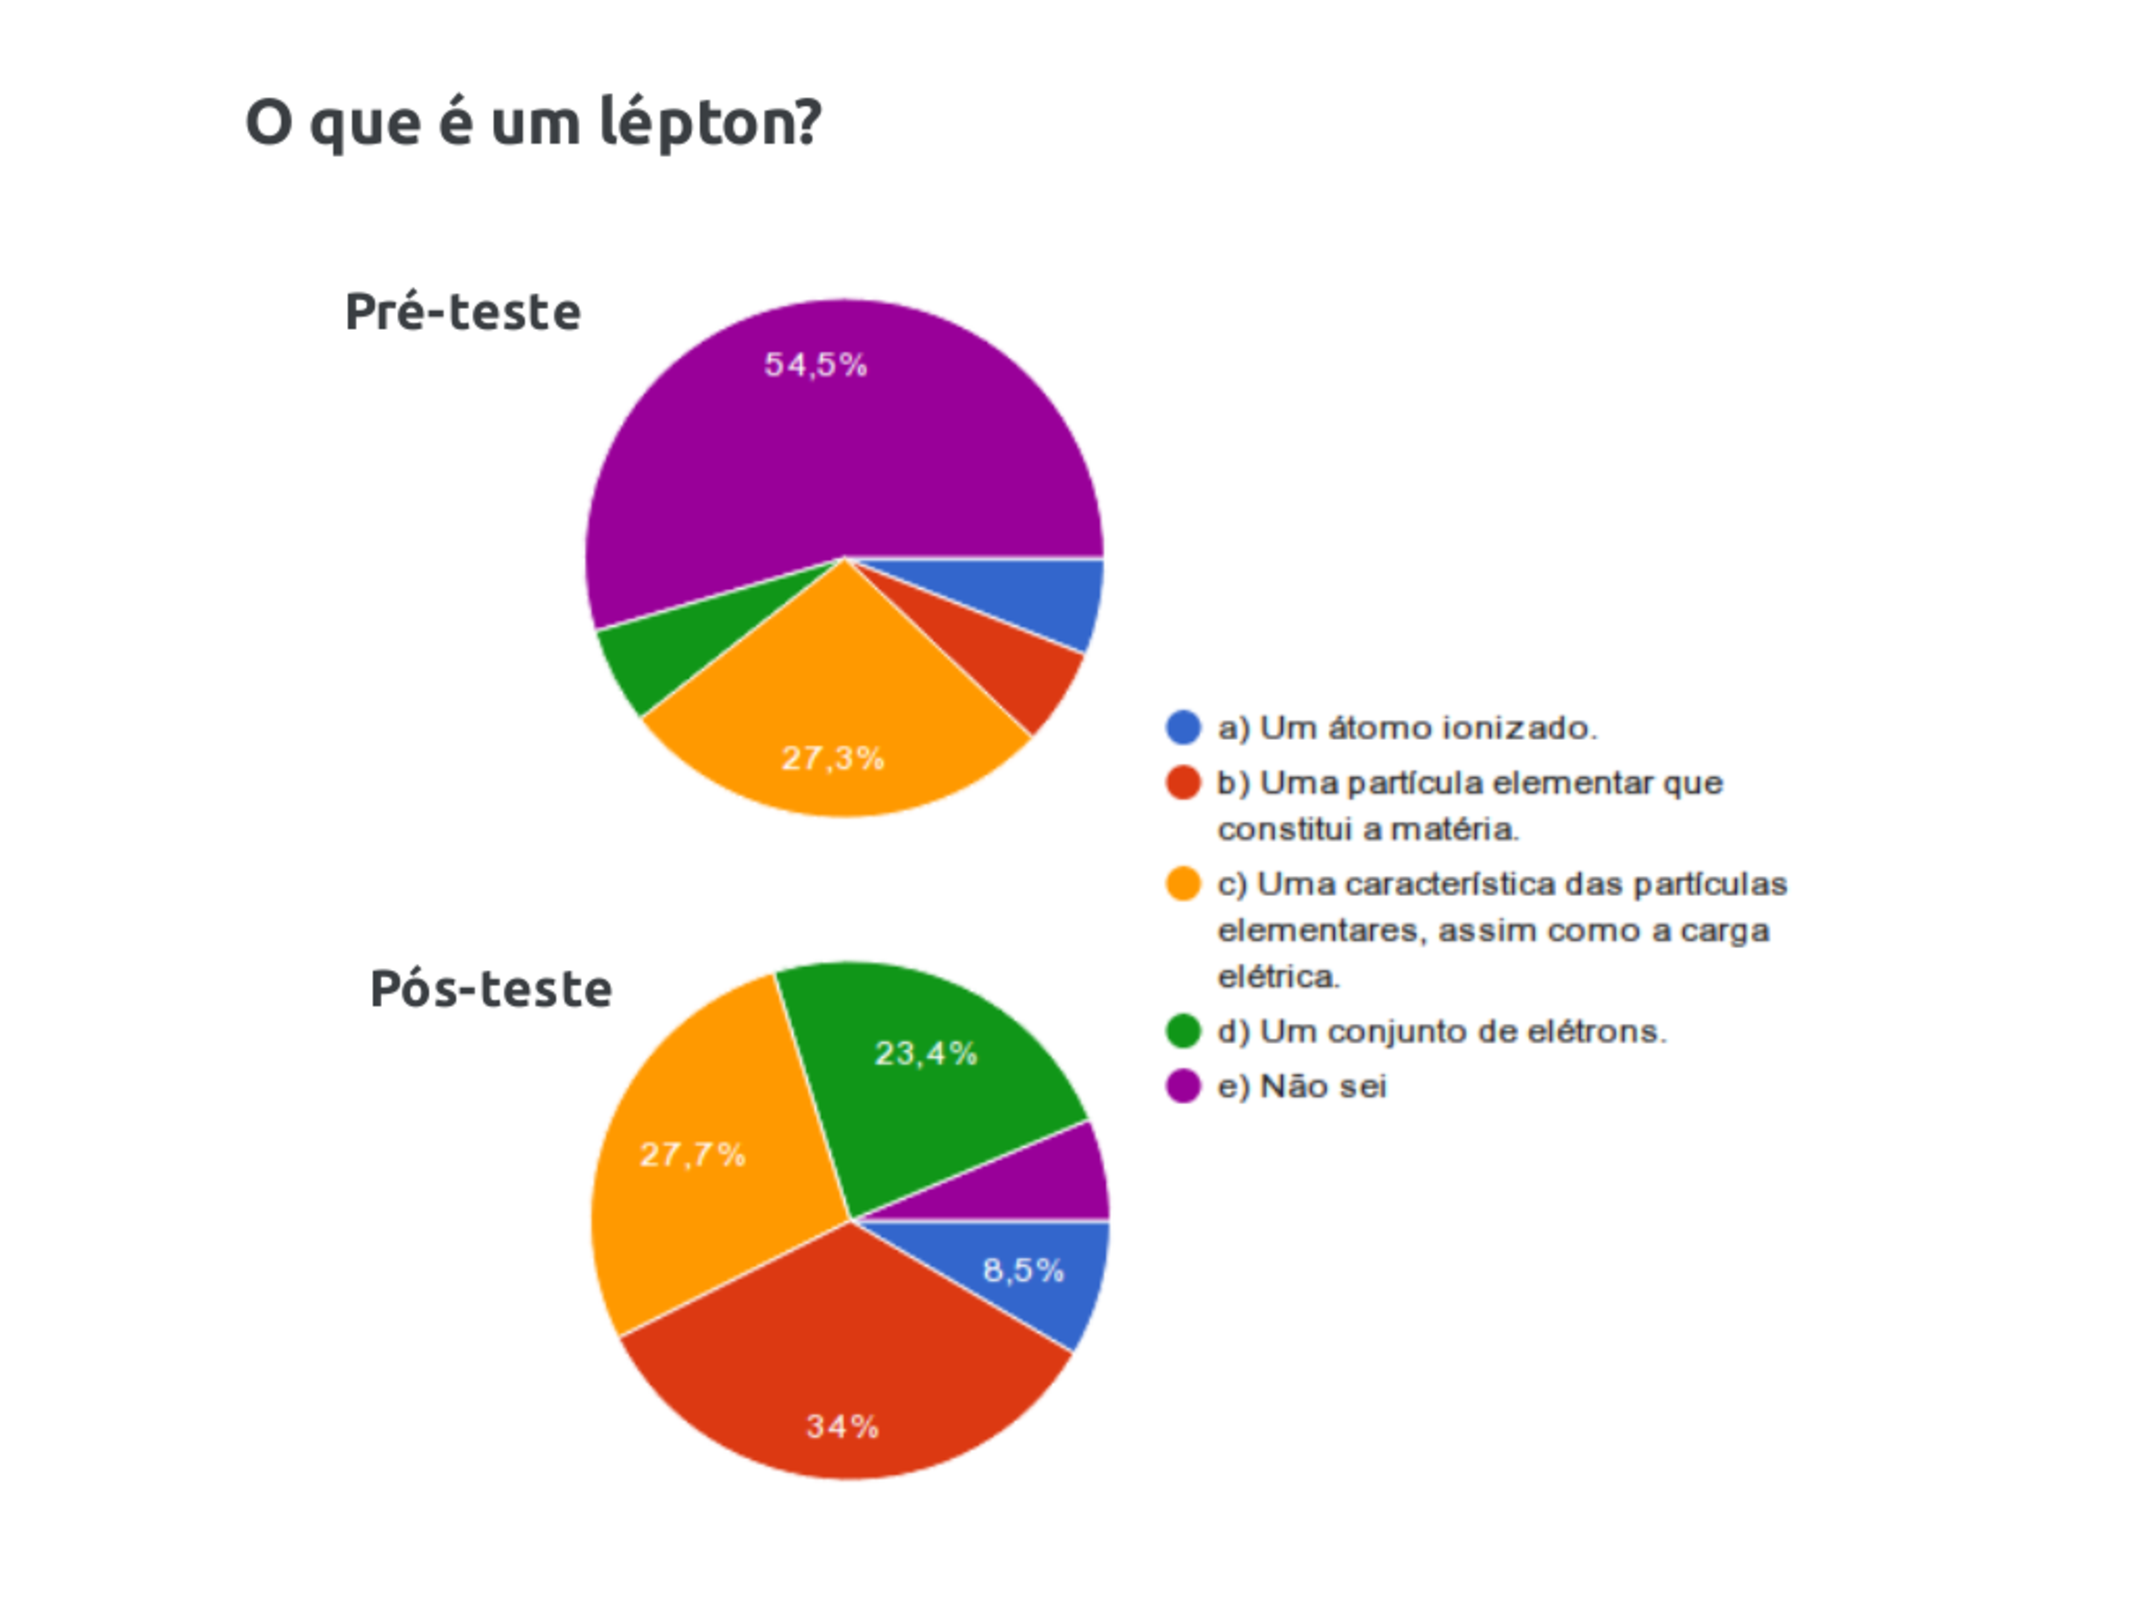
\includegraphics[width=0.72 \textwidth]{Resultados_e_Discussoes/Teste/q13_1}
	\caption{Resultado dos Testes - Pergunta 12}
	\label{appb_fig:test_res_perg12}
\end{grafico}

\newpage

\begin{grafico}[ht]
	\centering
	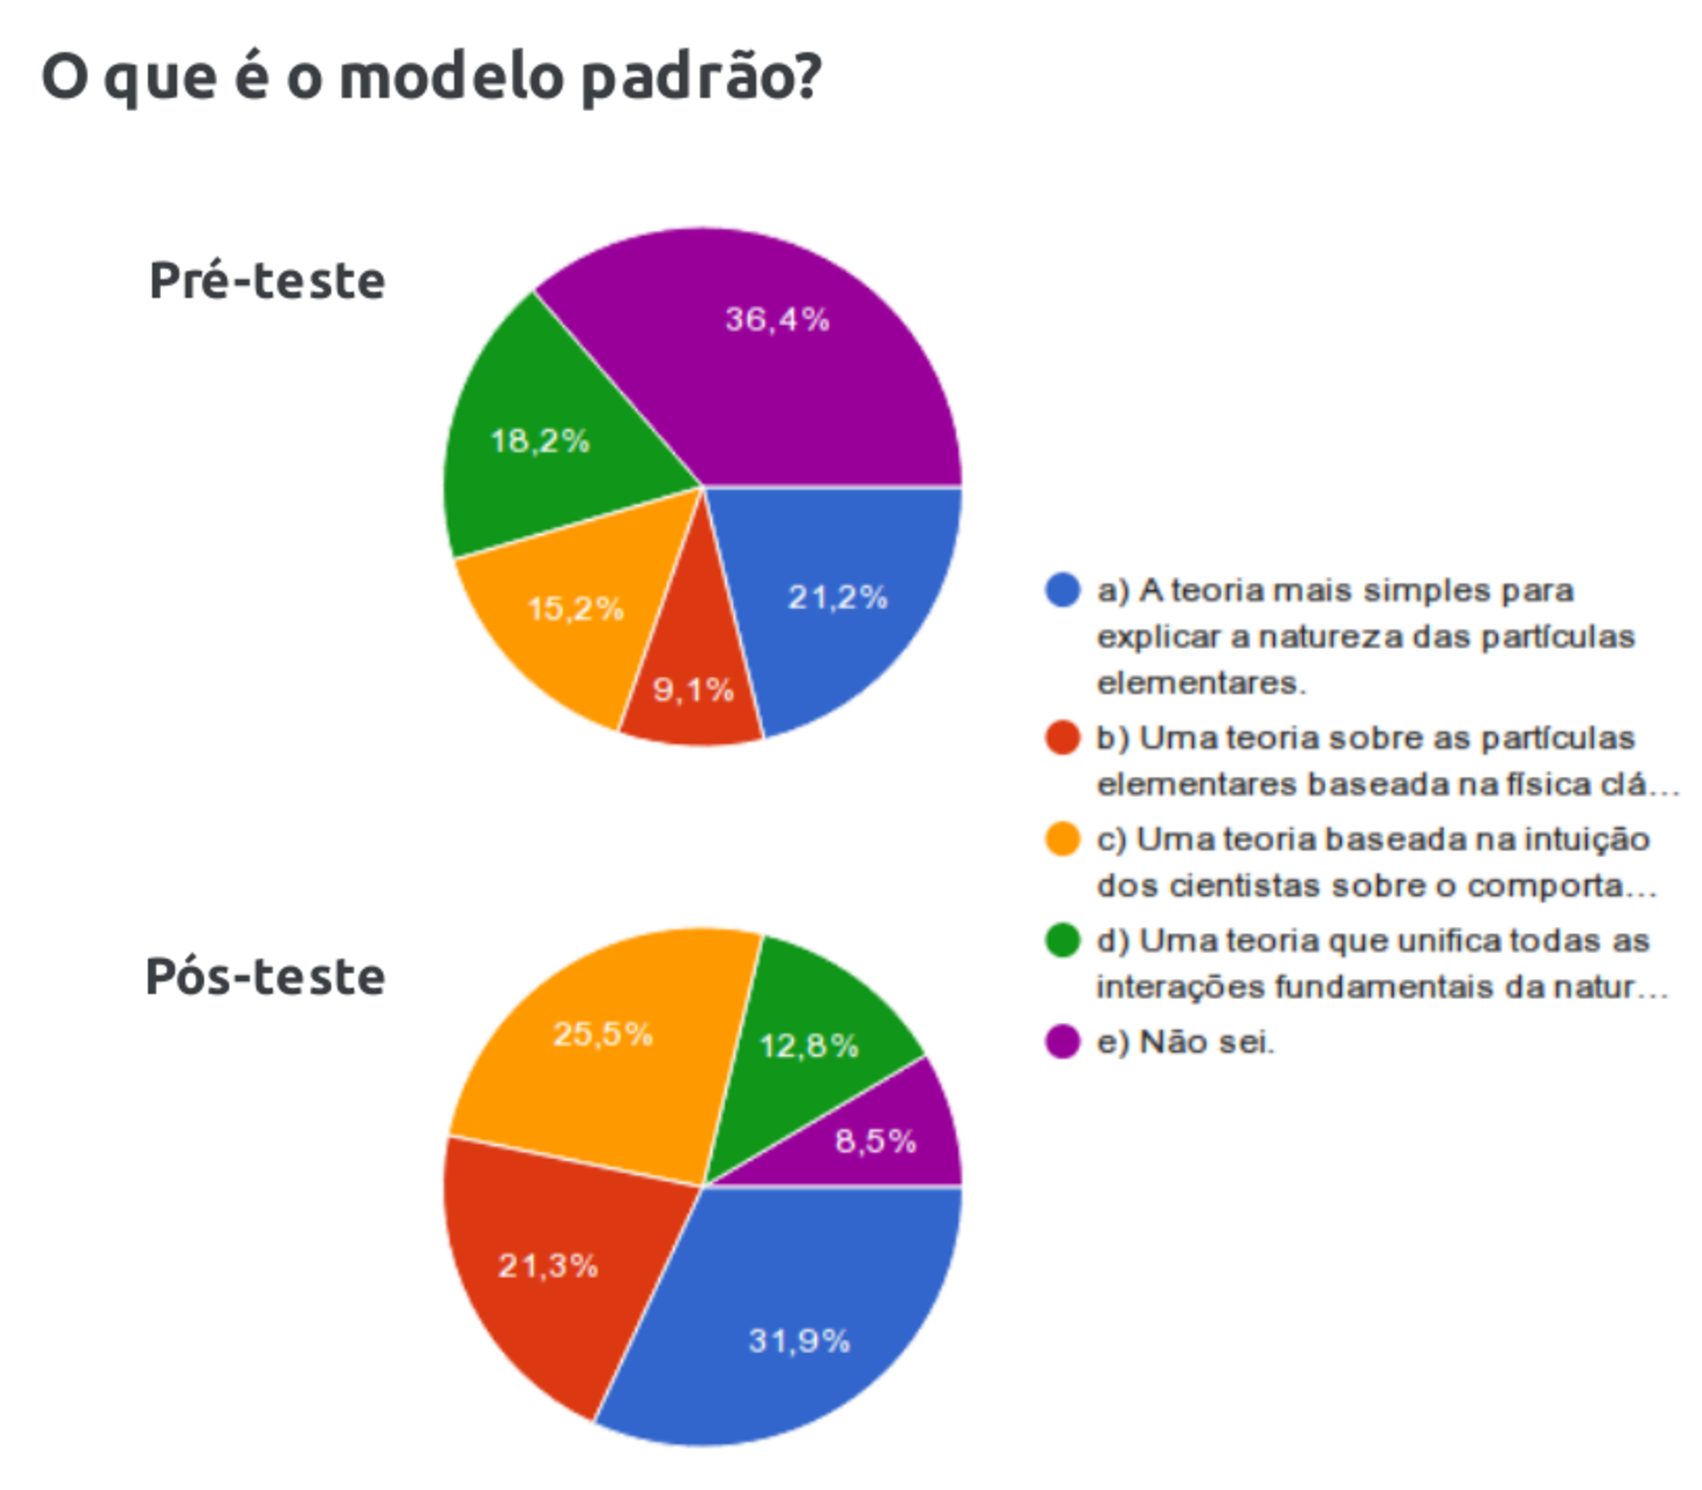
\includegraphics[width=0.58 \textwidth]{Resultados_e_Discussoes/Teste/q14_1}
	\caption{Resultado dos Testes - Pergunta 13}
	\label{appb_fig:test_res_perg13}
\end{grafico}

\begin{grafico}[ht]
	\centering
	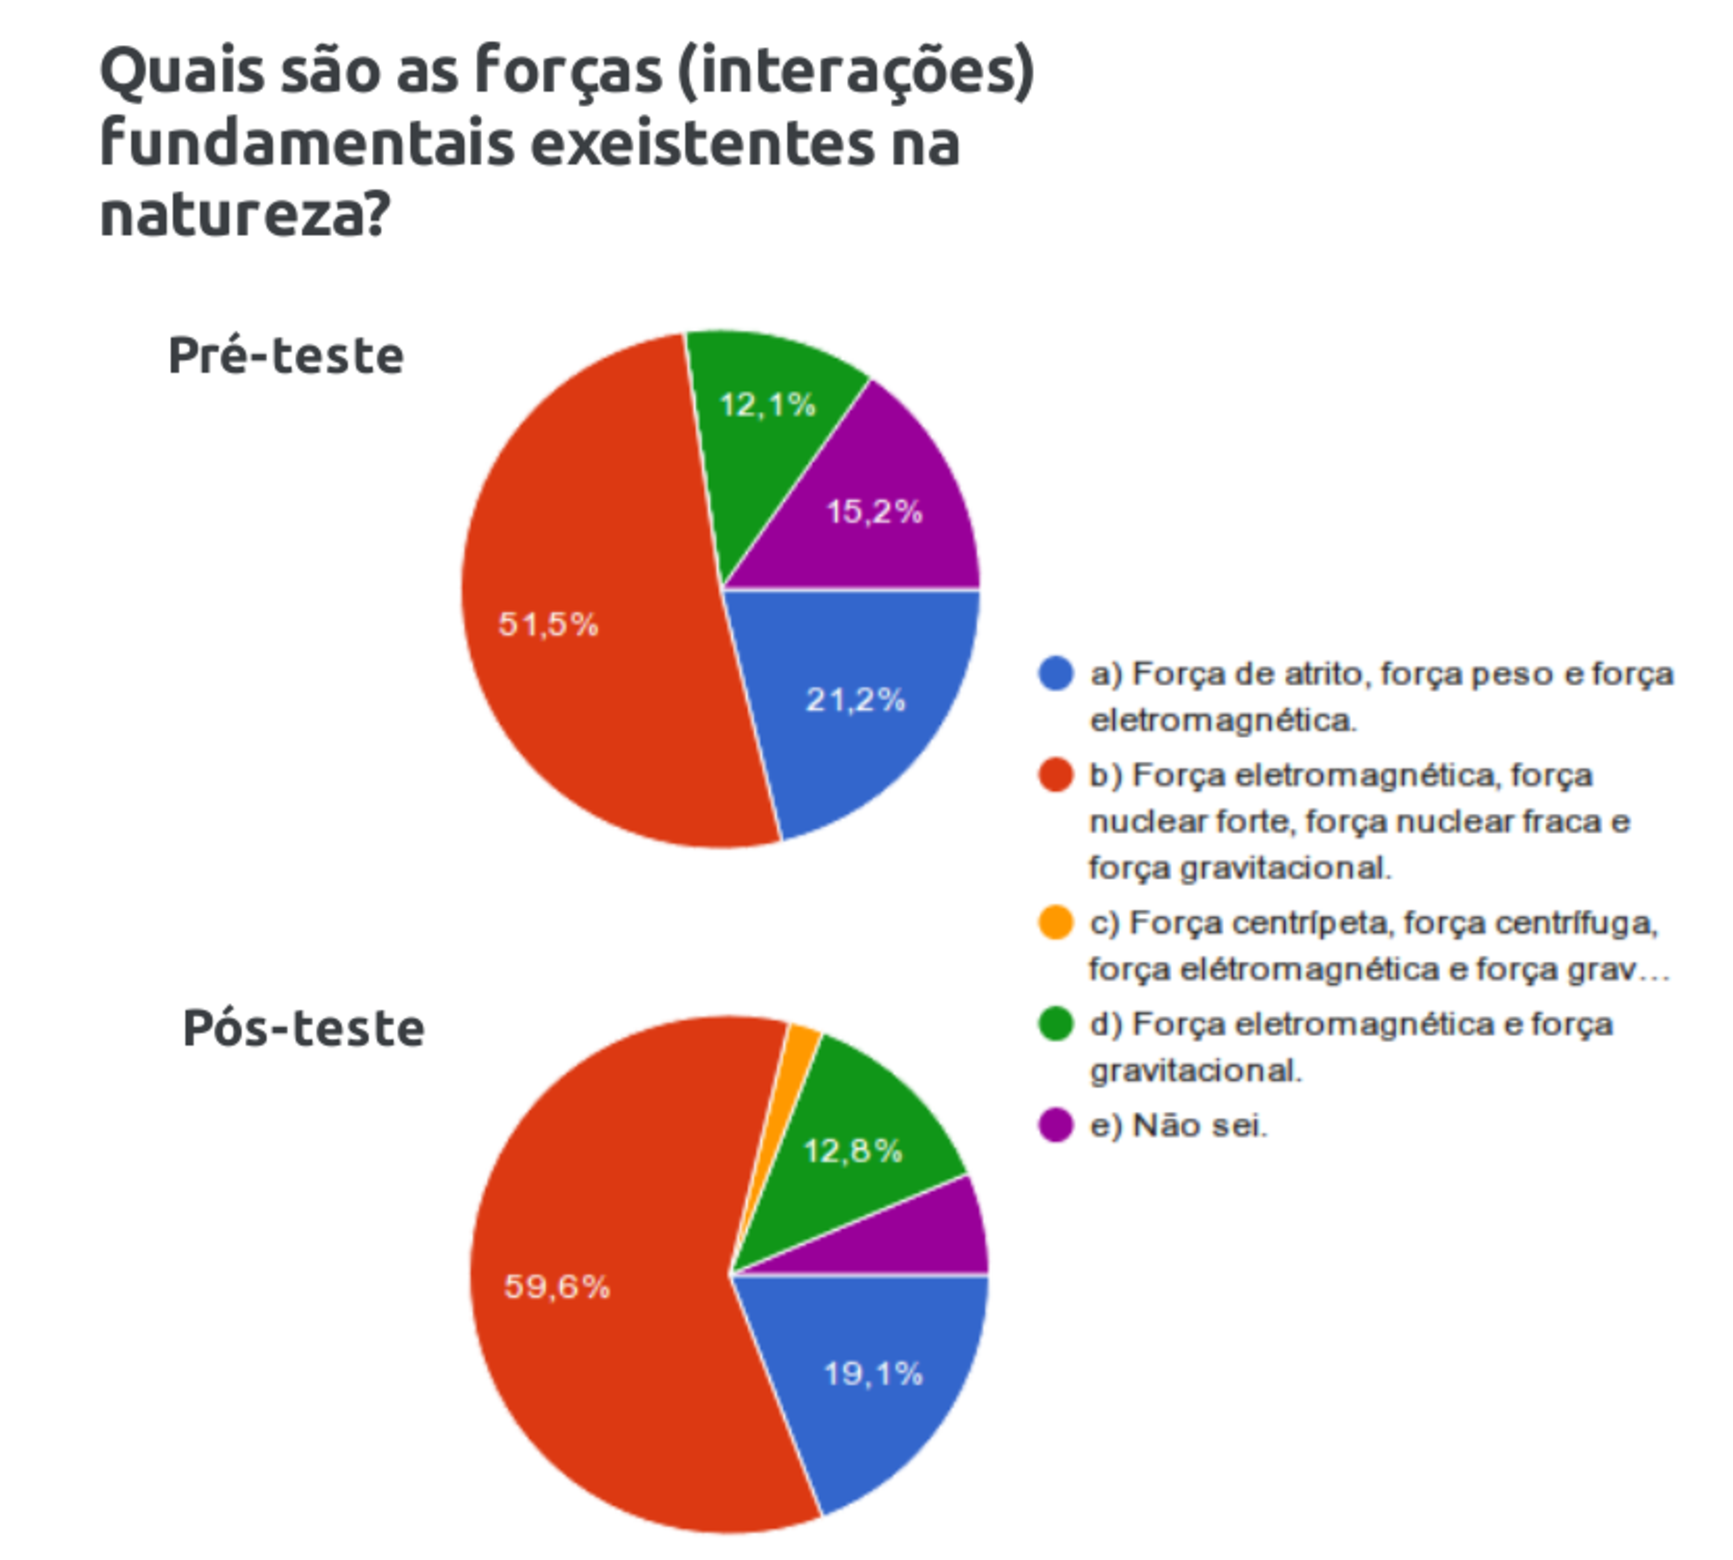
\includegraphics[width=0.58 \textwidth]{Resultados_e_Discussoes/Teste/q16_1}
	\caption{Resultado dos Testes - Pergunta 14}
	\label{appb_fig:test_res_perg14}
\end{grafico}

\newpage

\begin{grafico}[ht]
	\centering
	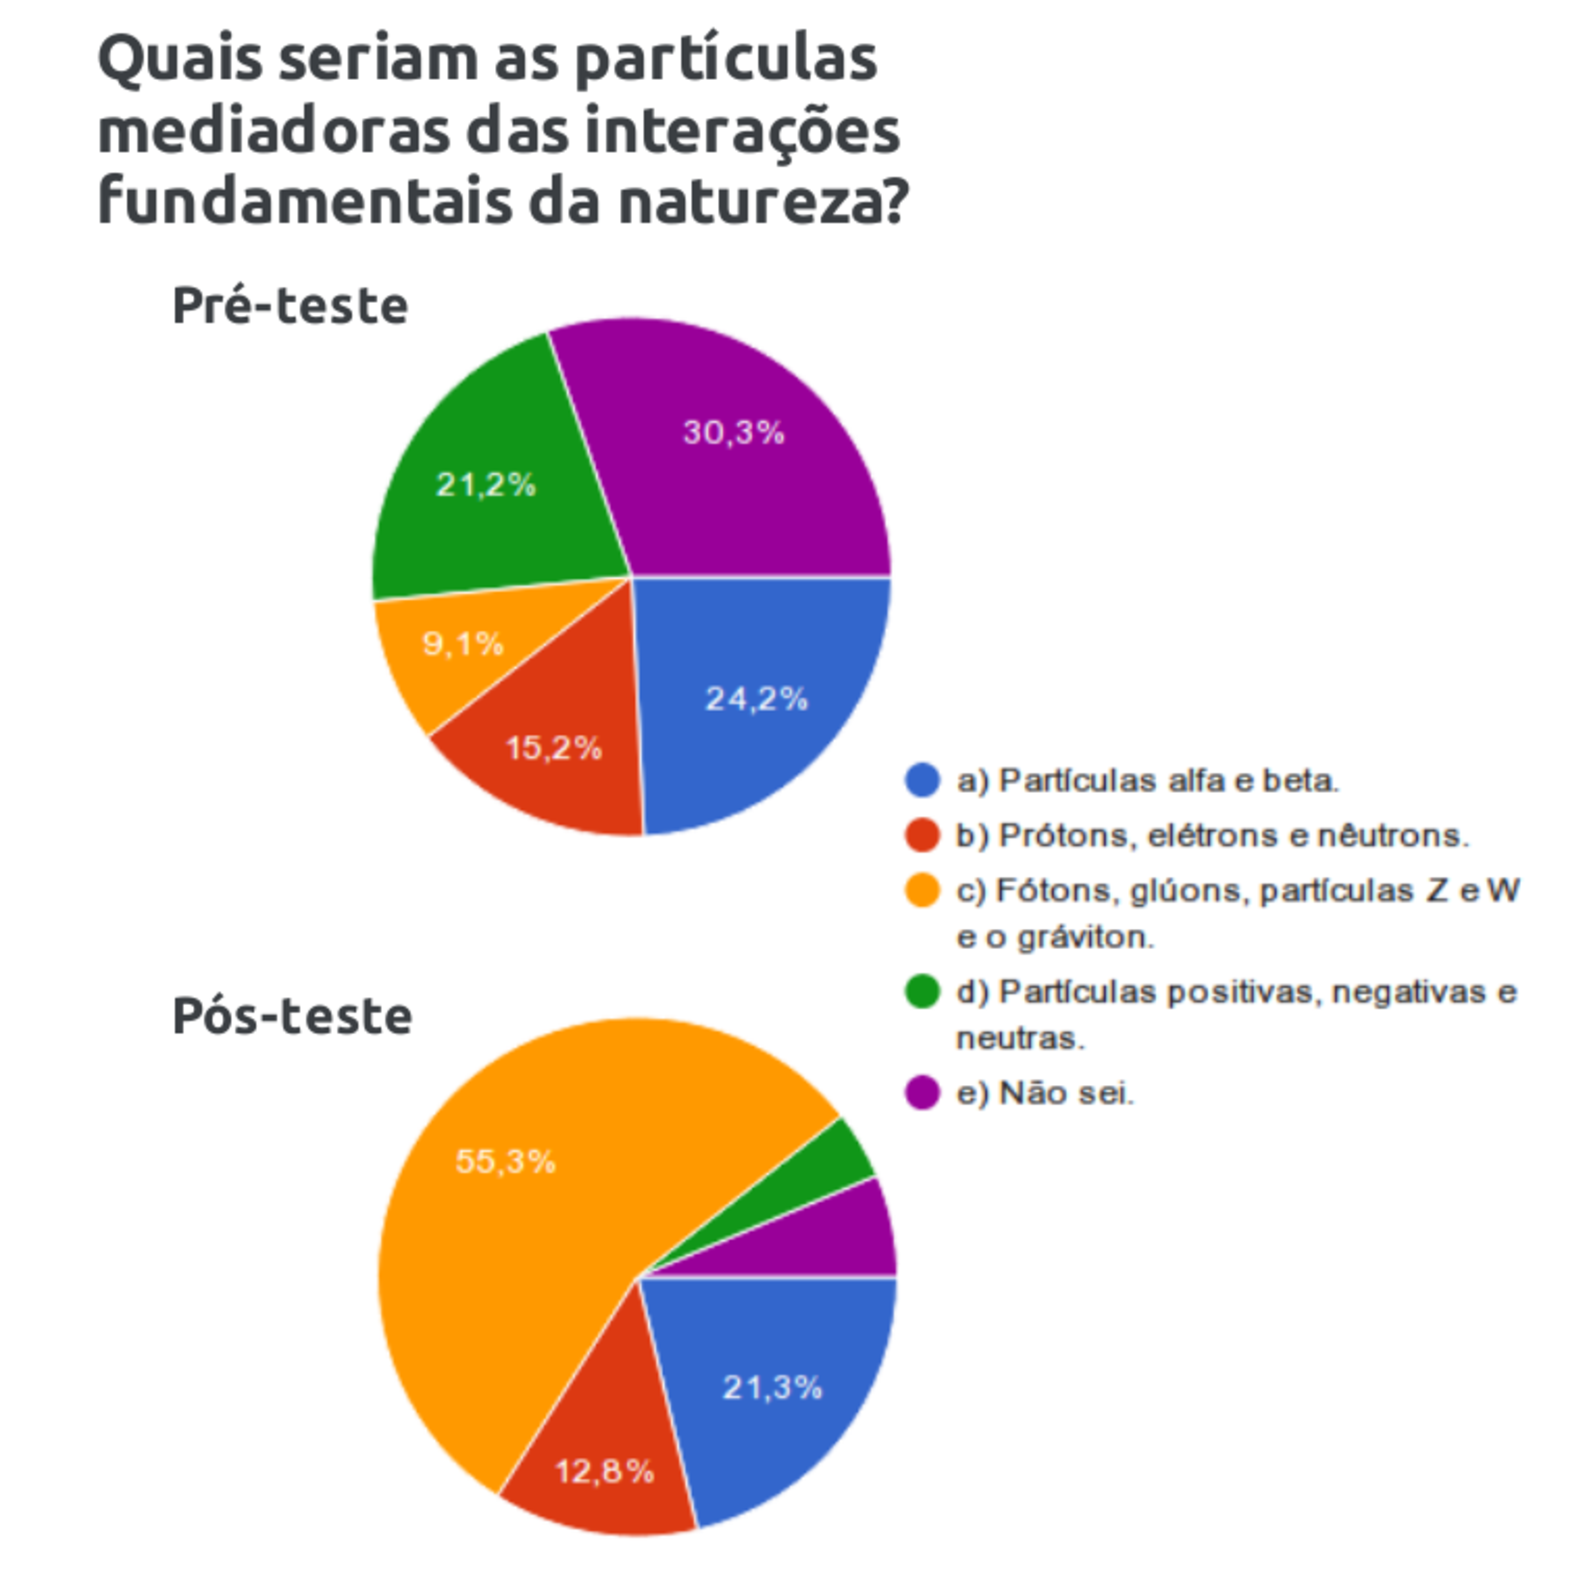
\includegraphics[width=0.52 \textwidth]{Resultados_e_Discussoes/Teste/q17_1}
	\caption{Resultado dos Testes - Pergunta 15}
	\label{appb_fig:test_res_perg15}
\end{grafico}

\begin{grafico}[ht]
	\centering
	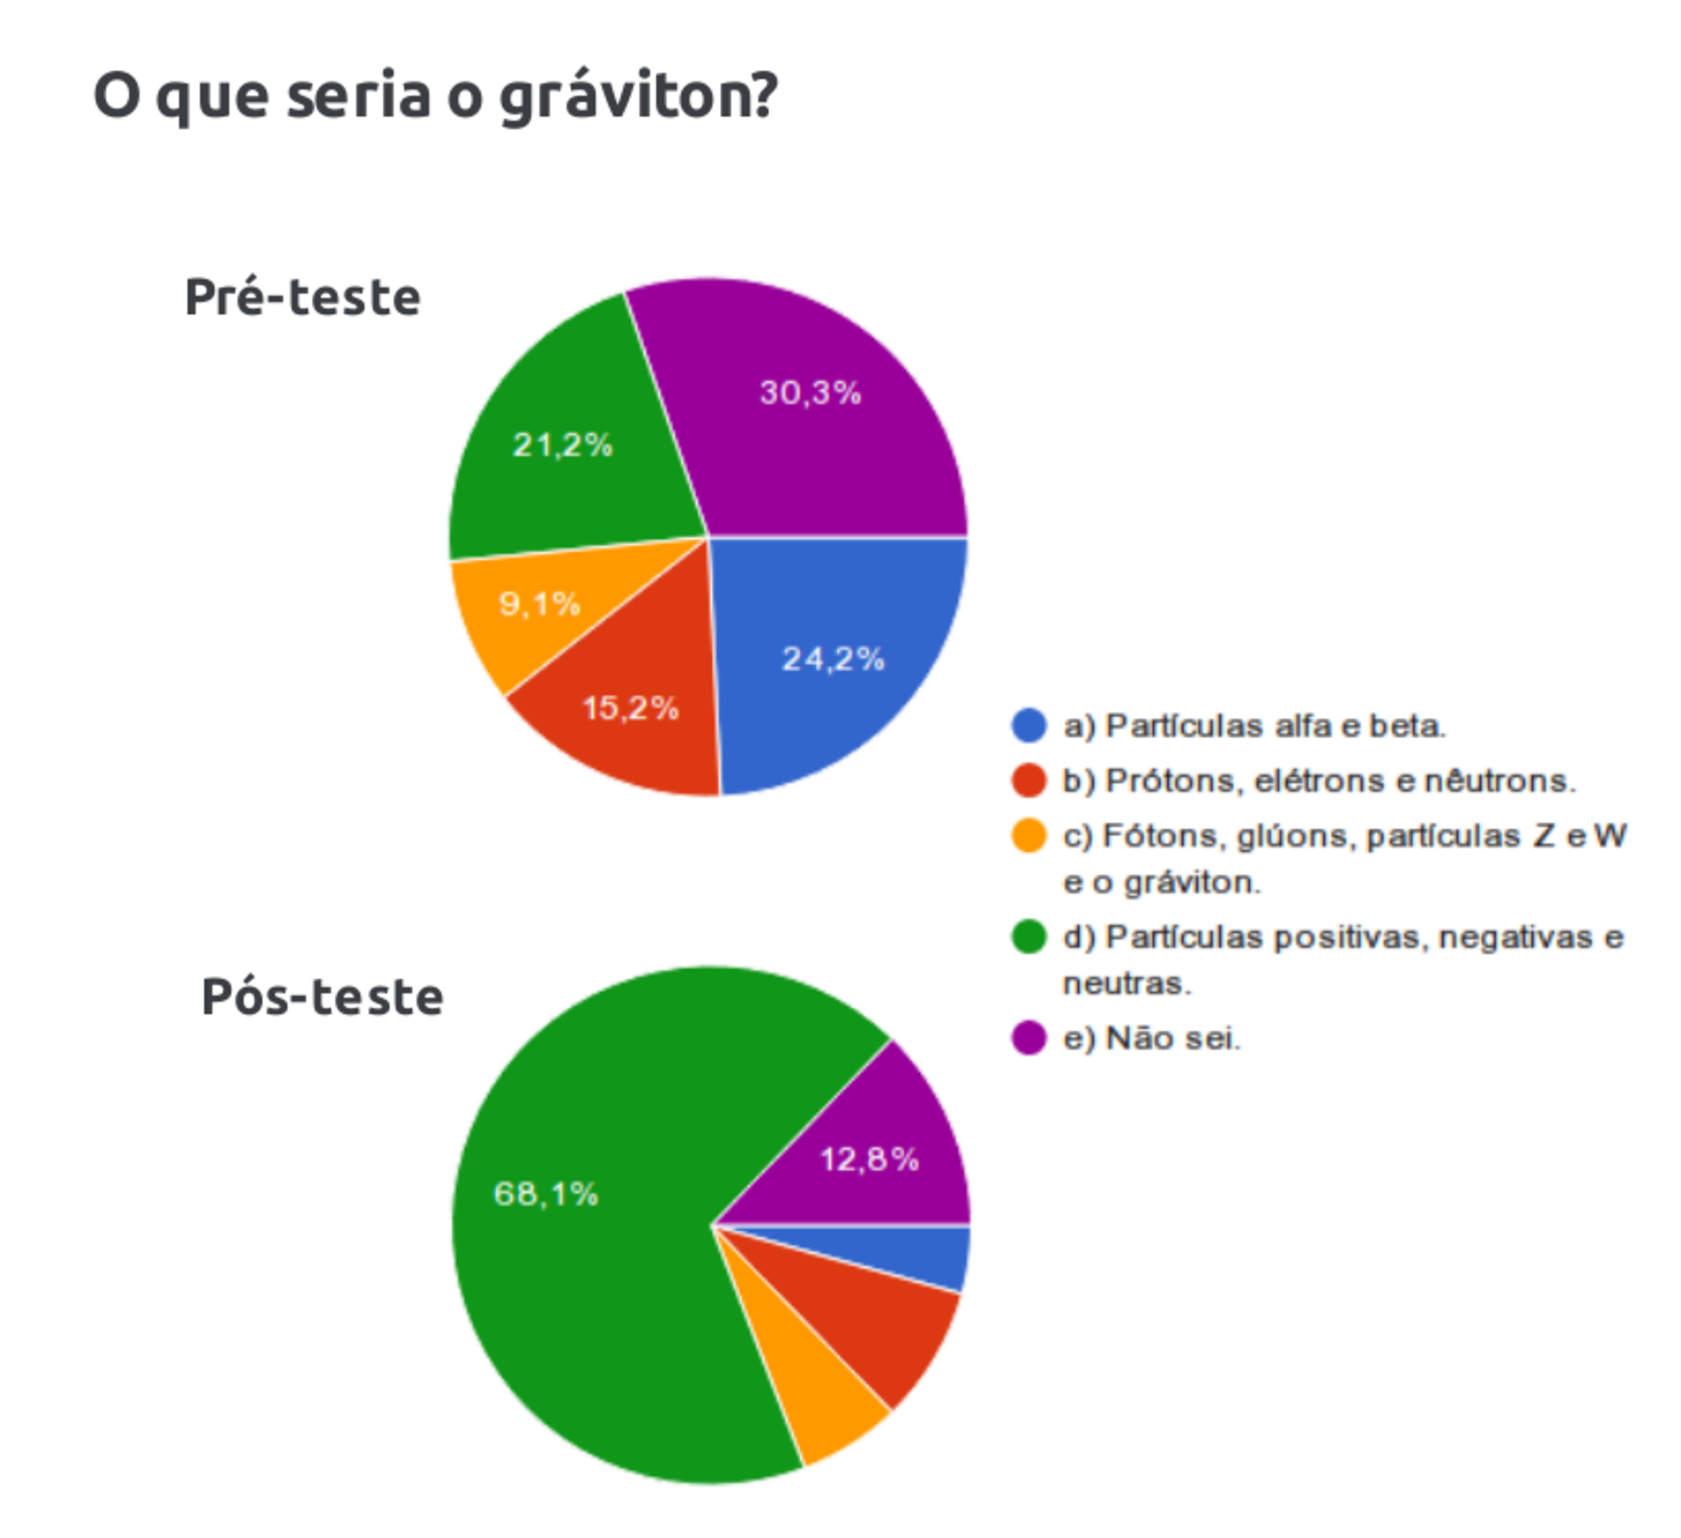
\includegraphics[width=0.57 \textwidth]{Resultados_e_Discussoes/Teste/q18_1}
	\caption{Resultado dos Testes - Pergunta 16}
	\label{appb_fig:test_res_perg16}
\end{grafico}

\newpage

\begin{grafico}[ht]
	\centering
	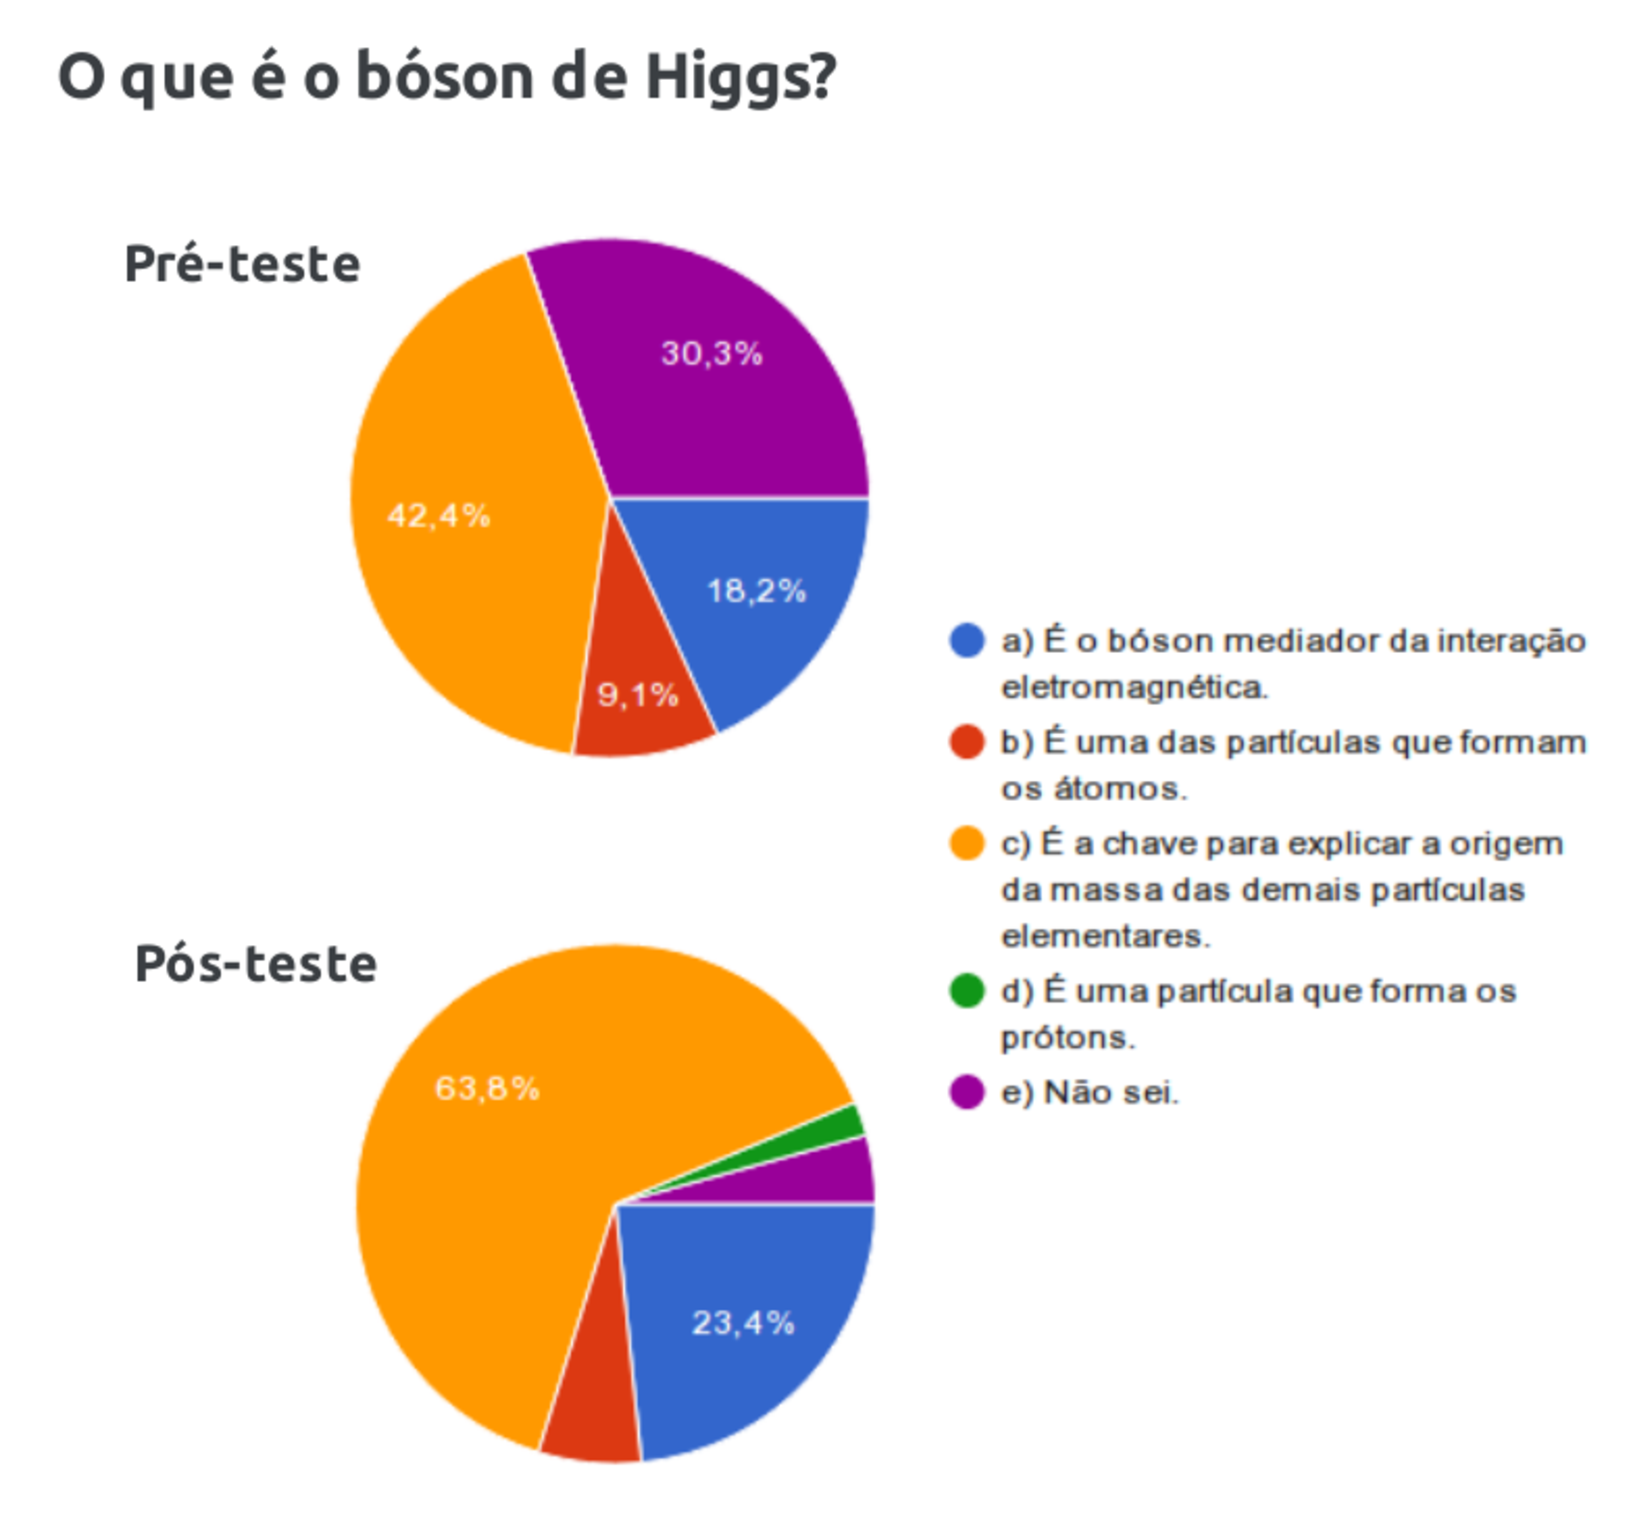
\includegraphics[width=0.58 \textwidth]{Resultados_e_Discussoes/Teste/q19_1}
	\caption{Resultado dos Testes - Pergunta 17}
	\label{appb_fig:test_res_perg17}
\end{grafico}

\begin{grafico}[ht]
	\centering
	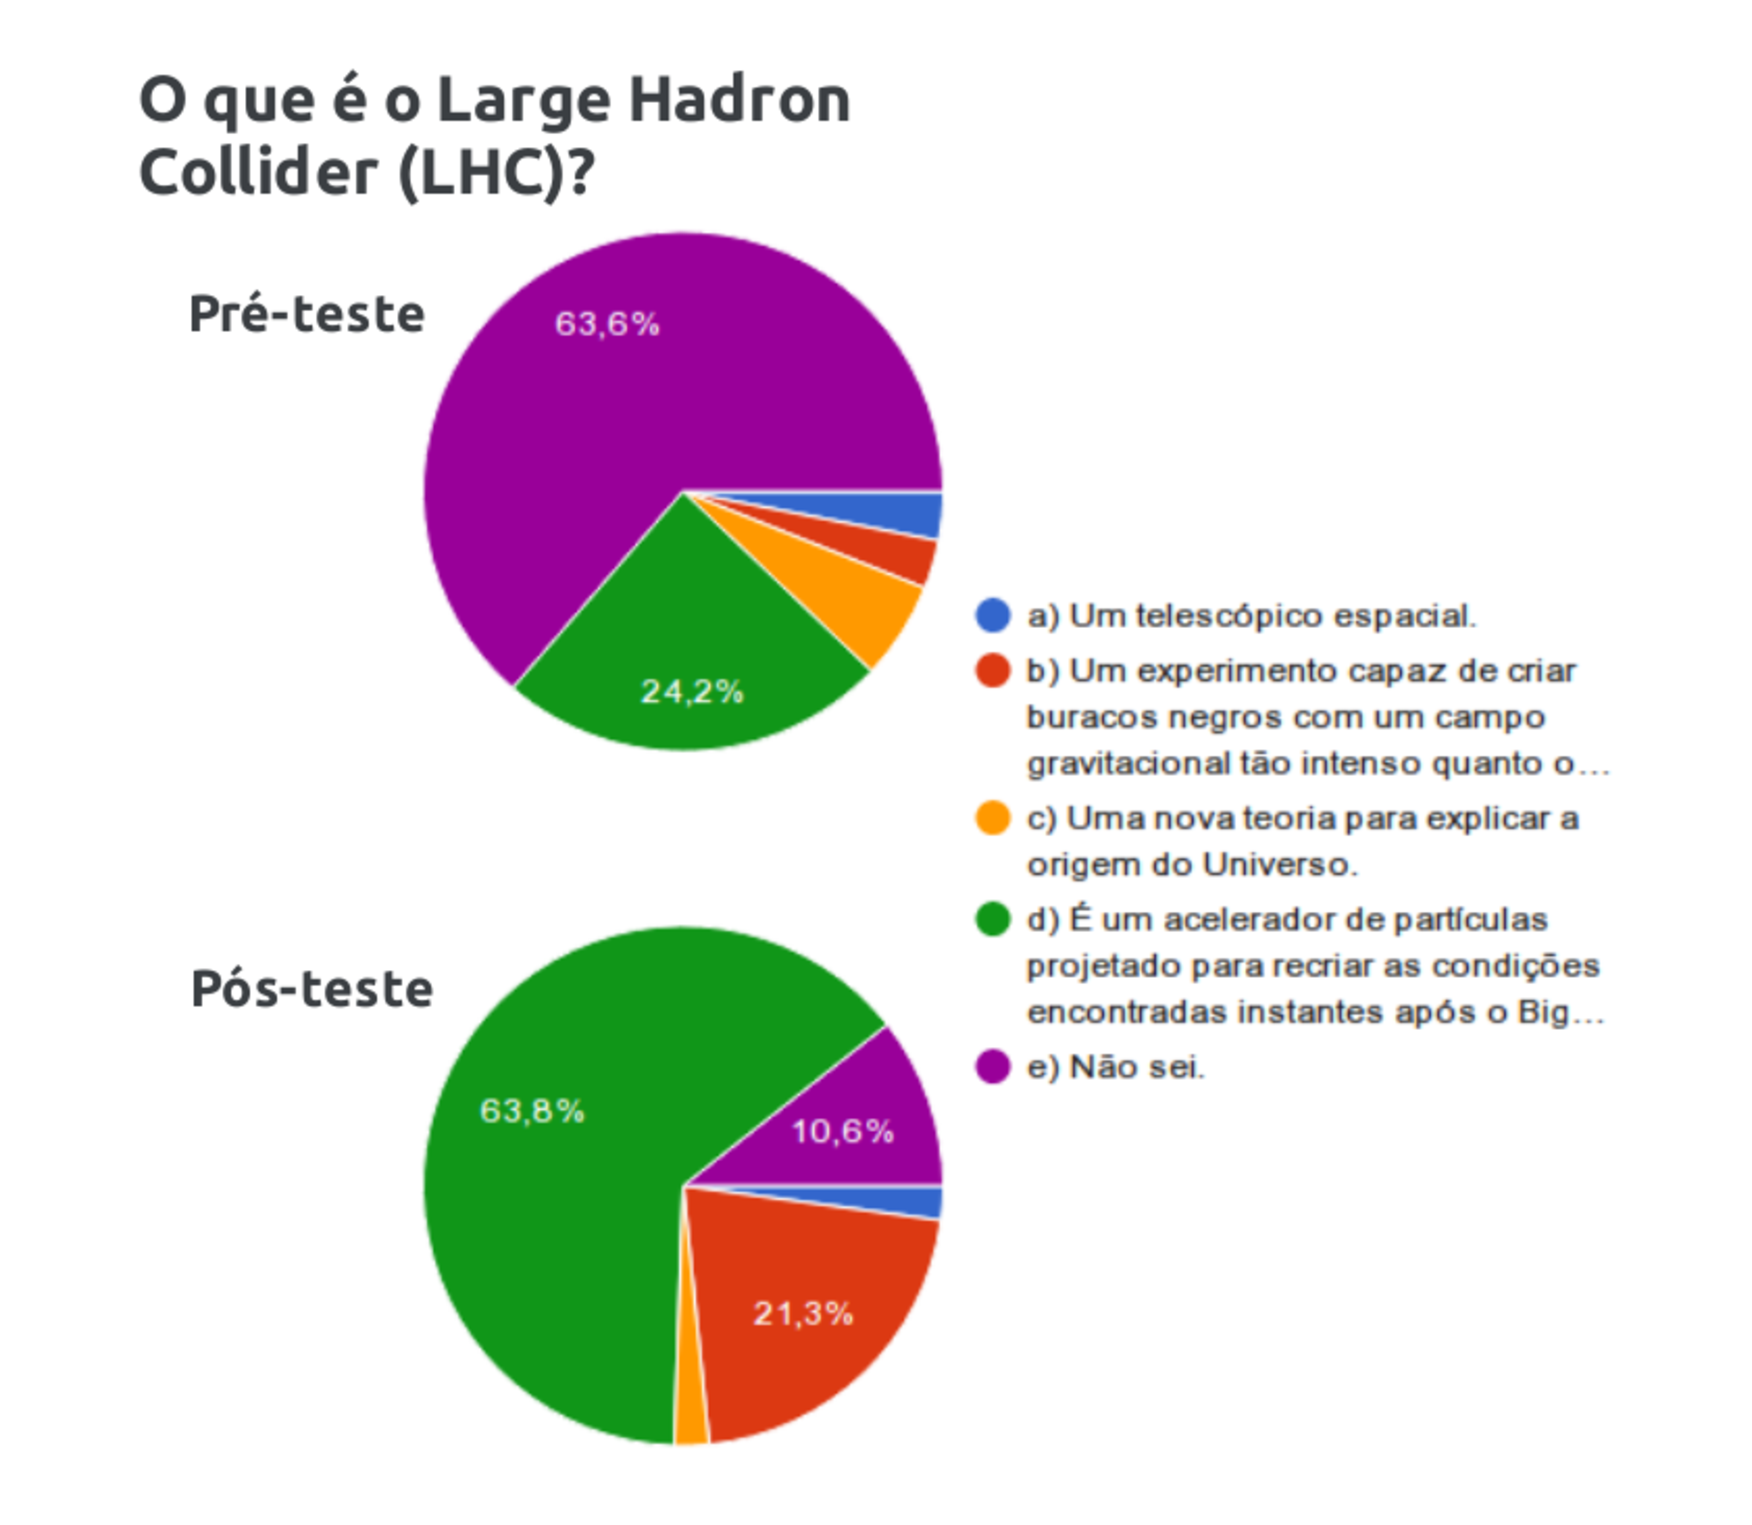
\includegraphics[width=0.58 \textwidth]{Resultados_e_Discussoes/Teste/q20_1}
	\caption{Resultado dos Testes - Pergunta 18}
	\label{appb_fig:test_res_perg18}
\end{grafico}

\newpage

\section{Pesquisa Final}\label{app_b:final}

\begin{figura}[h]
	\centering
	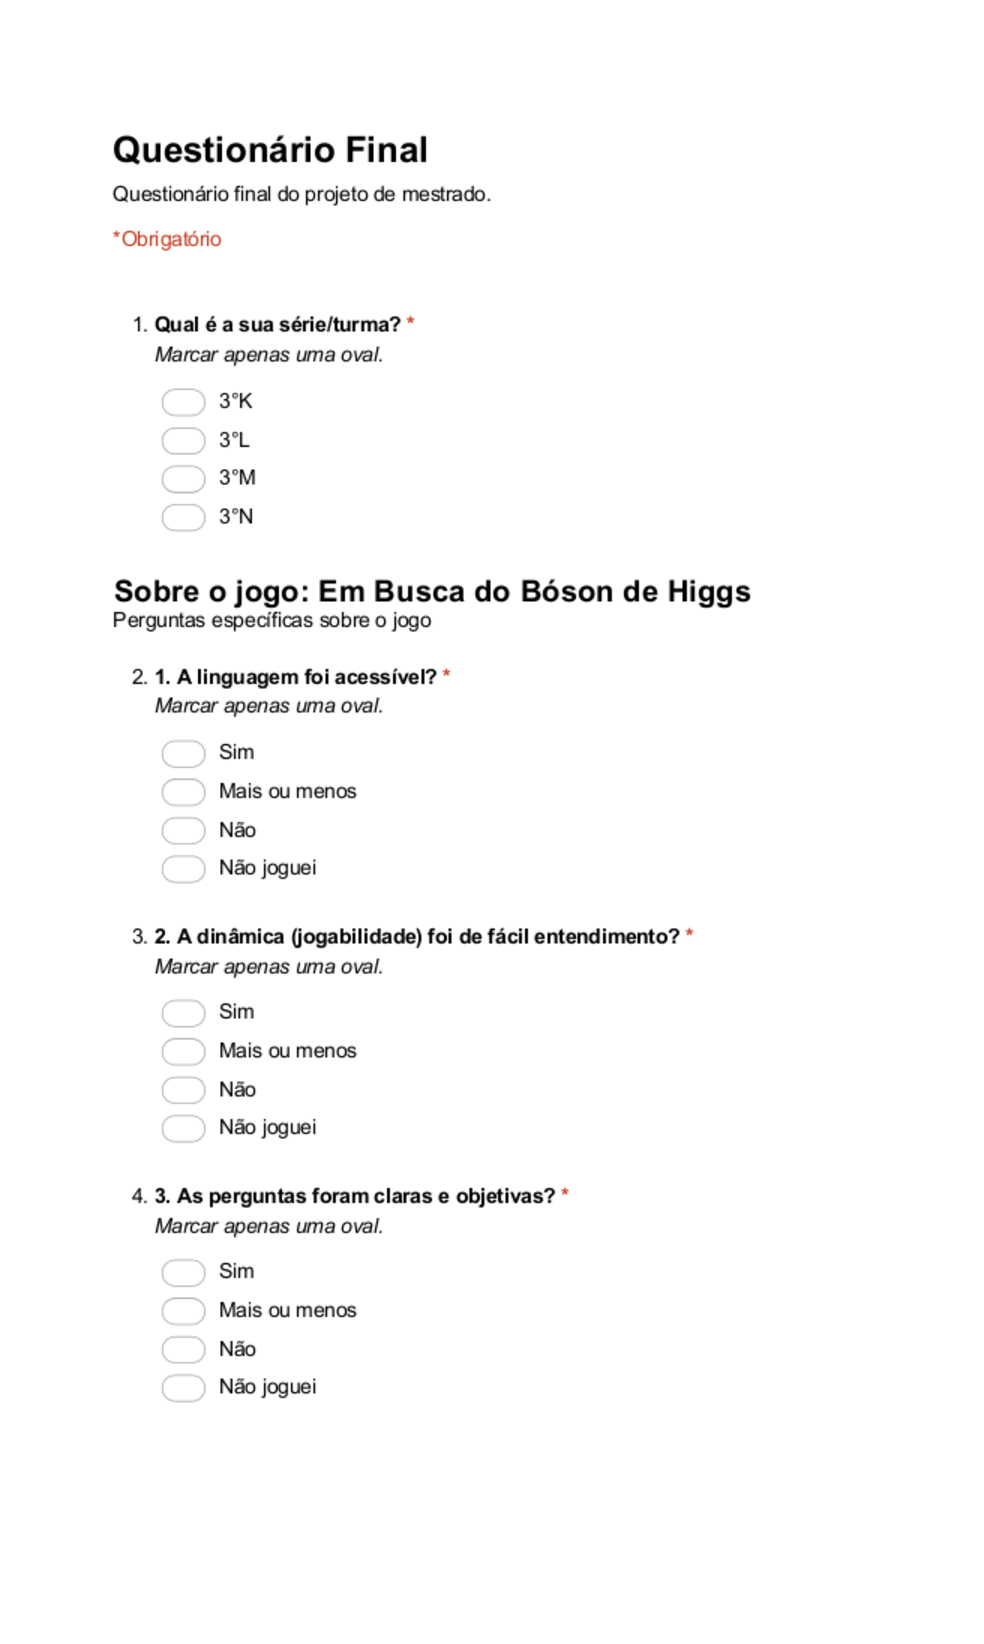
\includegraphics[width=0.69 \textwidth]{ApeB/Img_pesq_fin/pf_part1}
	\caption{Pesquisa final: parte 1}
	\label{appb_fig:pf_part1}
\end{figura}

\newpage

\begin{figura}[h]
	\centering
	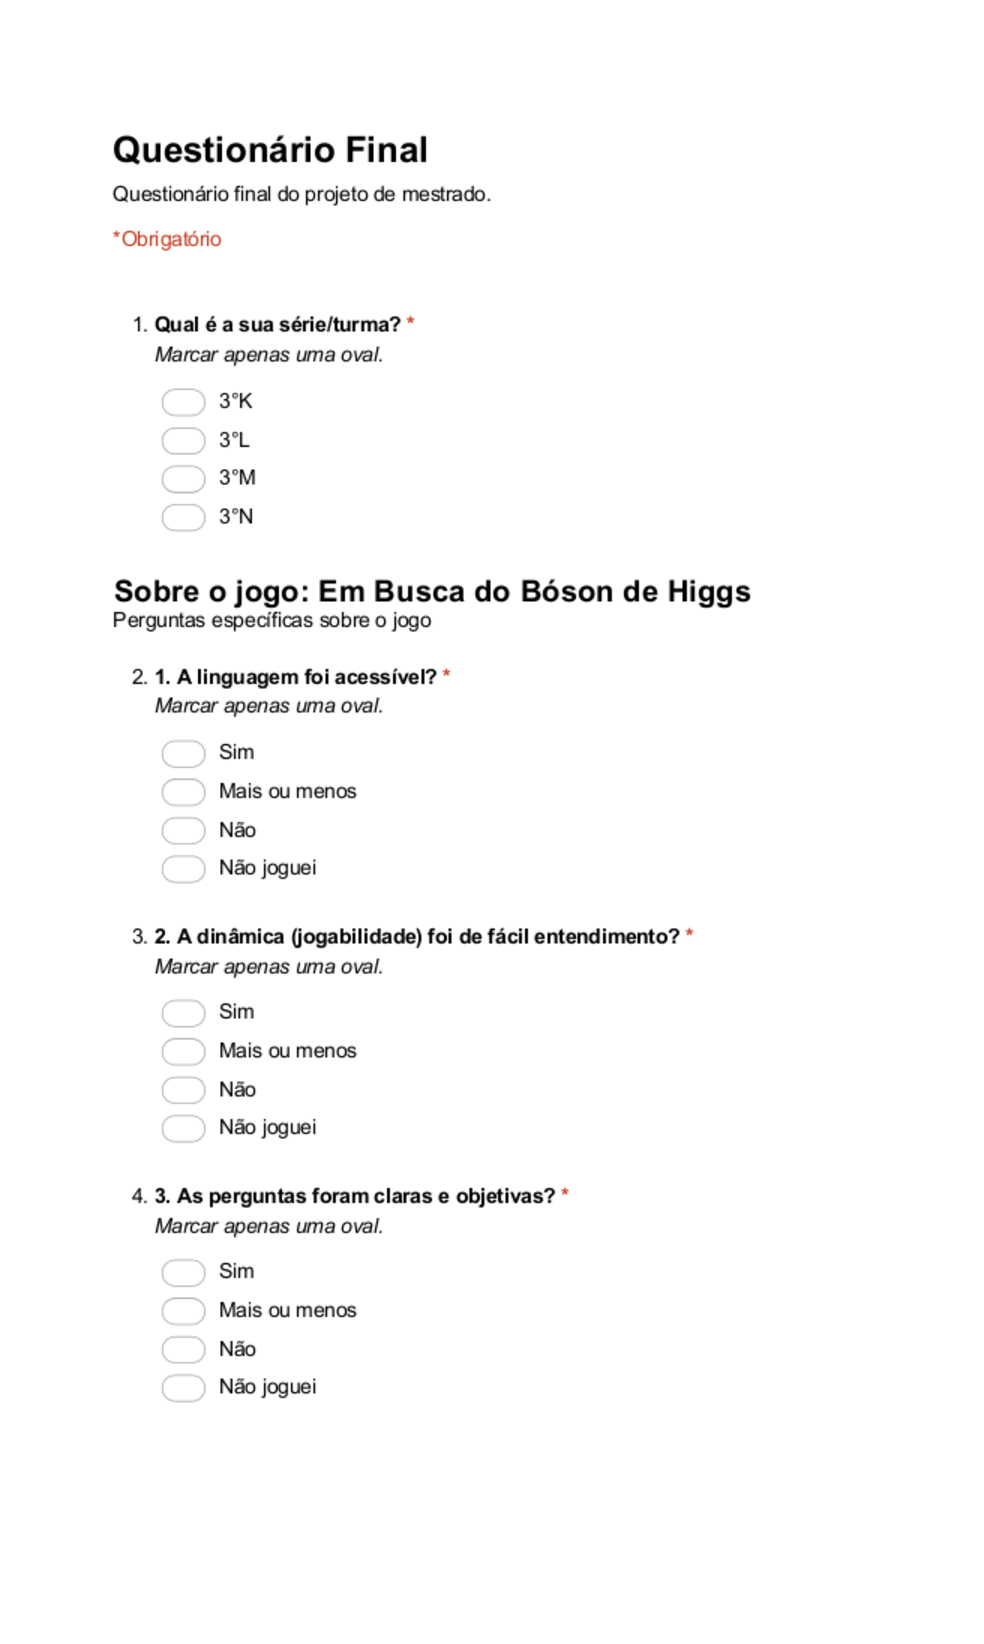
\includegraphics[width=0.69 \textwidth]{ApeB/Img_pesq_fin/pf_part1}
	\caption{Pesquisa final: parte 2}
	\label{appb_fig:pf_part2}
\end{figura}

\newpage

\begin{figura}[h]
	\centering
	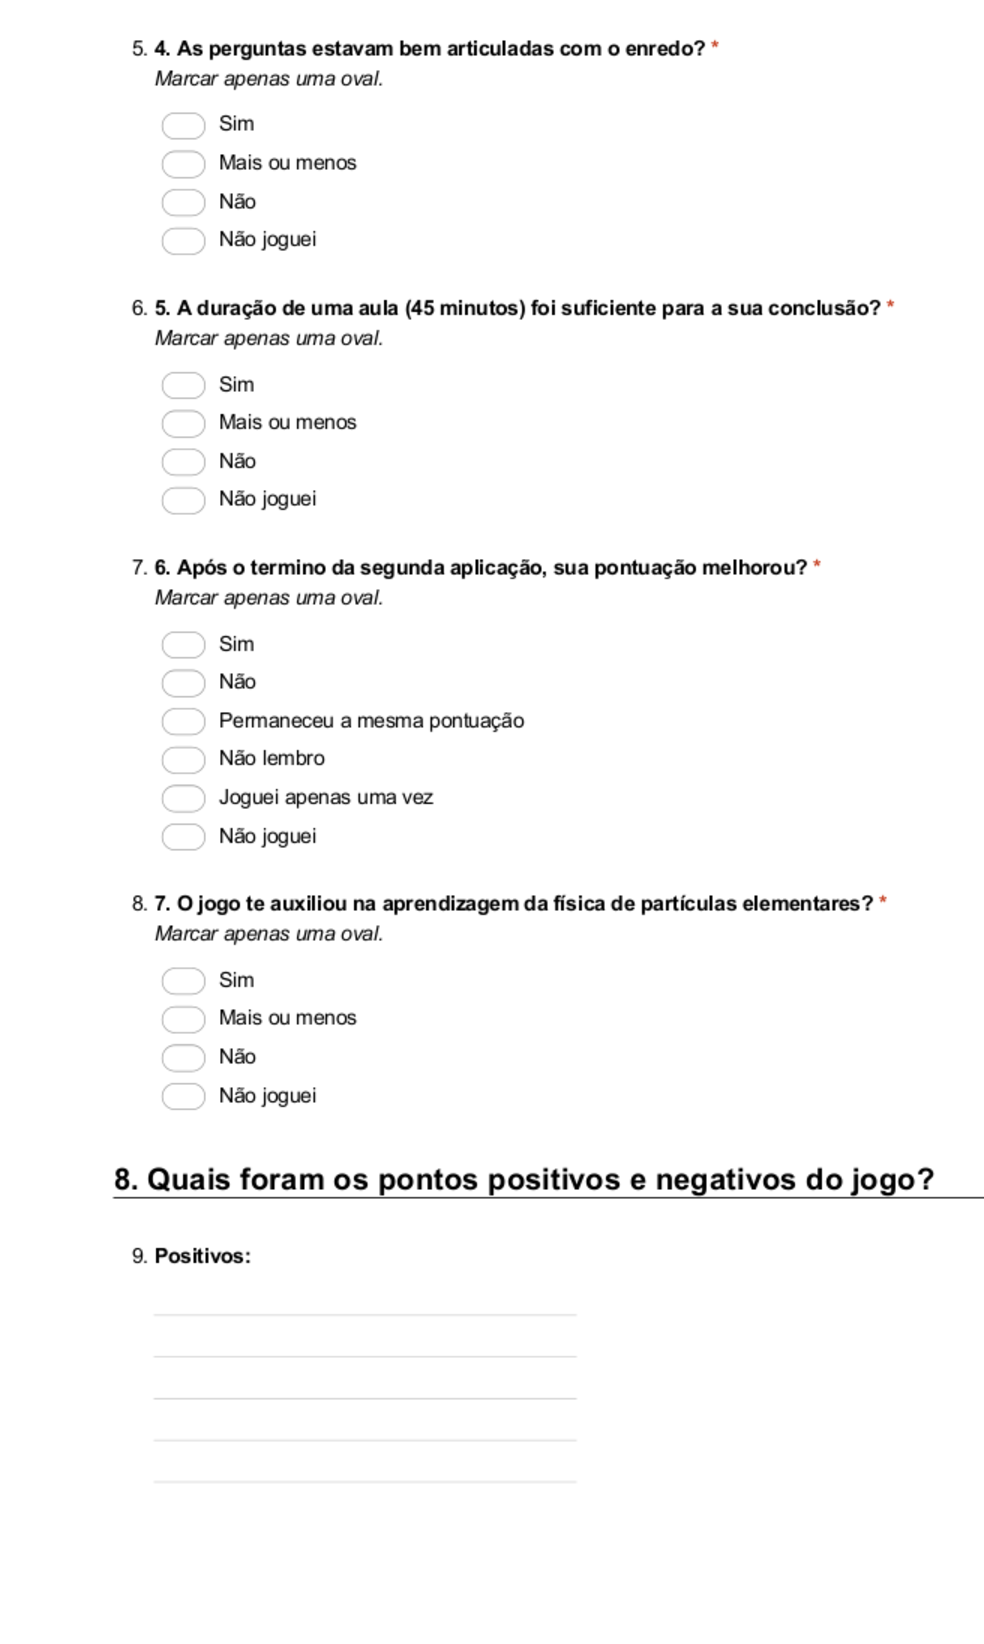
\includegraphics[width=0.69 \textwidth]{ApeB/Img_pesq_fin/pf_part2}
	\caption{Pesquisa final: parte 3}
	\label{appb_fig:pf_part3}
\end{figura}

\newpage

\begin{figura}[h]
	\centering
	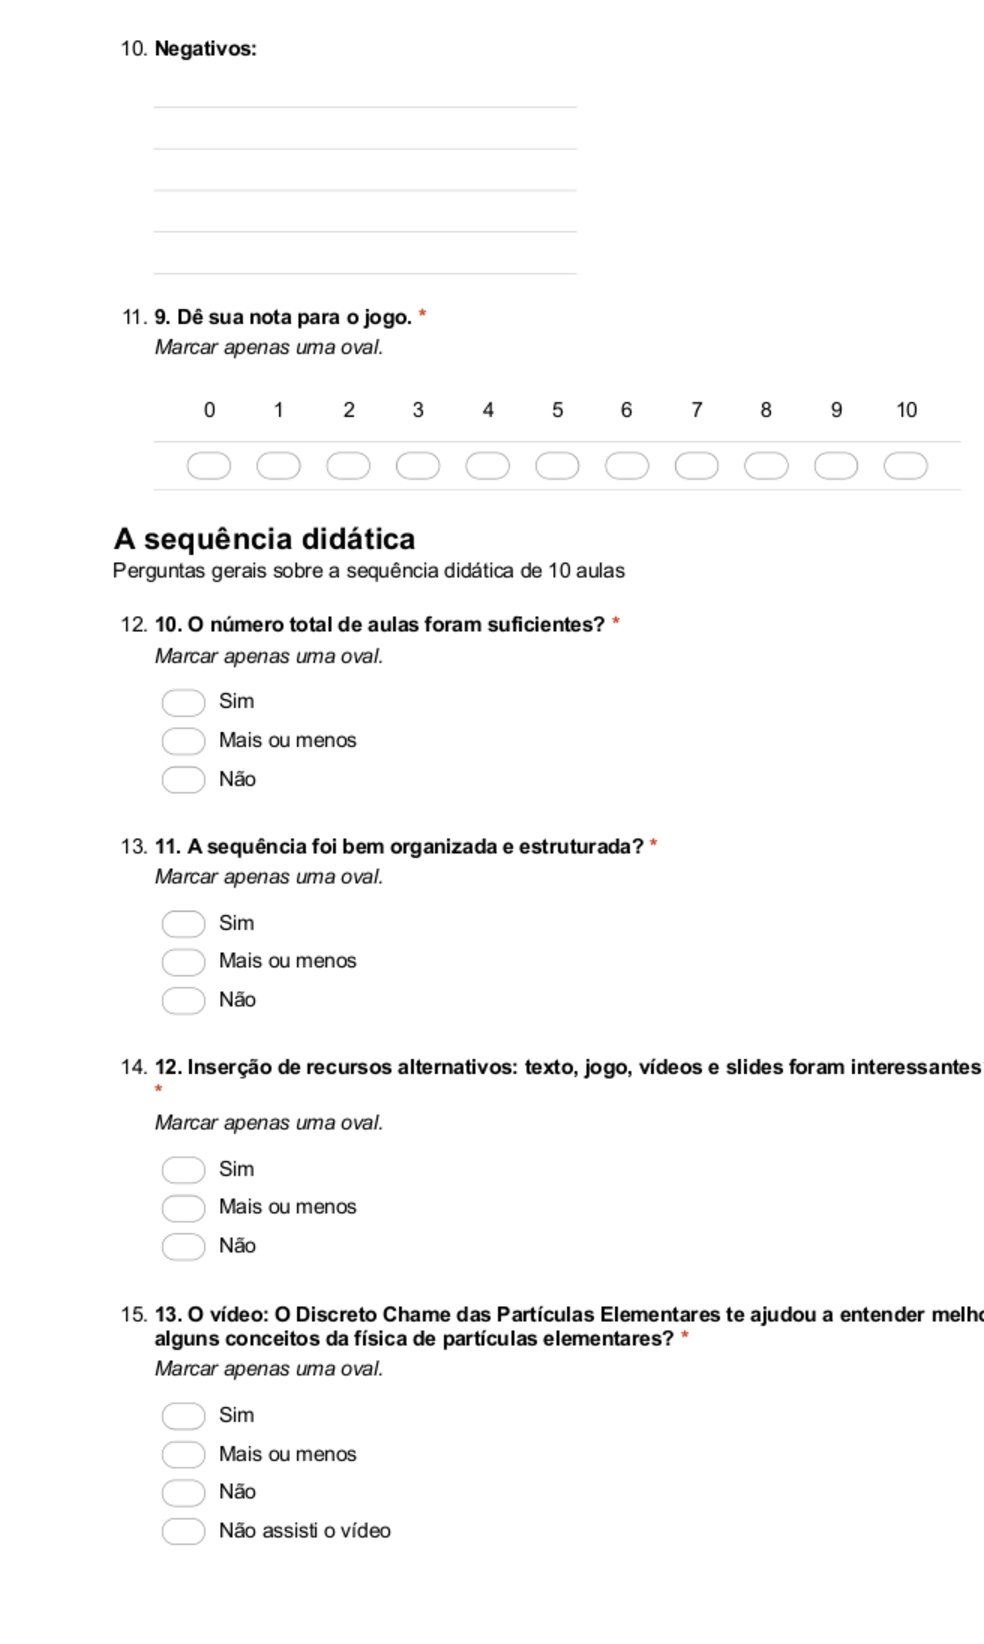
\includegraphics[width=0.69 \textwidth]{ApeB/Img_pesq_fin/pf_part3}
	\caption{Pesquisa final: parte 4}
	\label{appb_fig:pf_part4}
\end{figura}

\newpage

\begin{figura}[h]
	\centering
	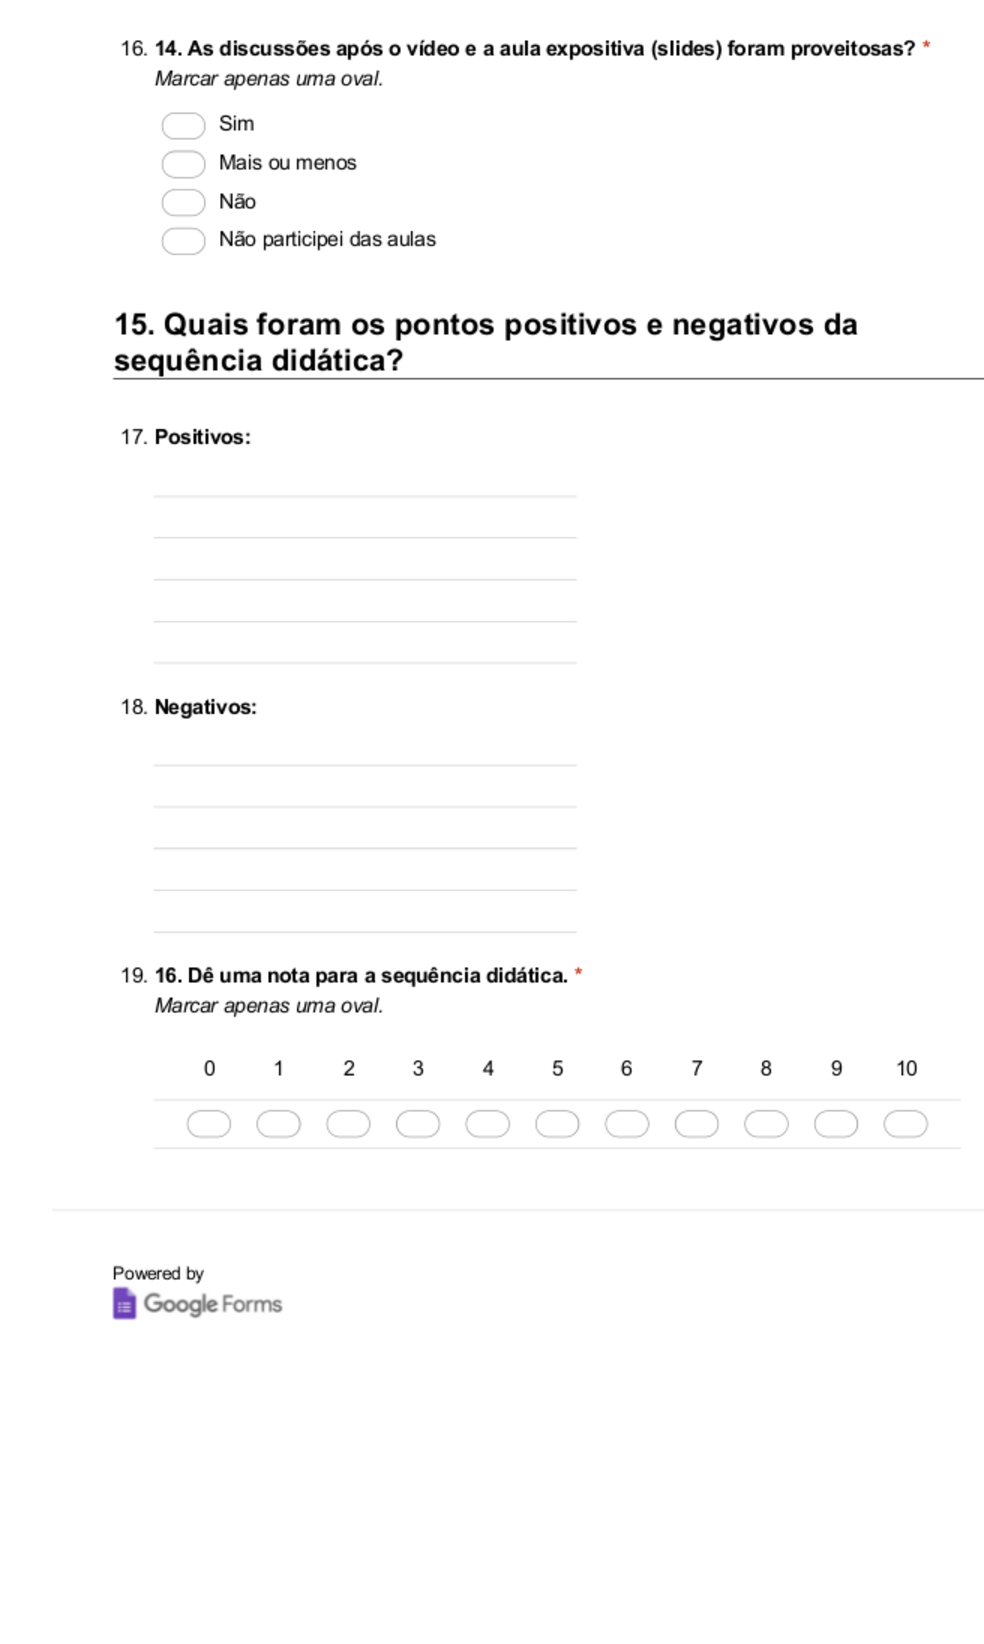
\includegraphics[width=0.69 \textwidth]{ApeB/Img_pesq_fin/pf_part4}
	\caption{Pesquisa final: parte 5}
	\label{appb_fig:pf_part5}
\end{figura}

\newpage

\section{Resultados da Pesquisa Final}\label{app_b:final}

\begin{grafico}[ht]
	\centering
	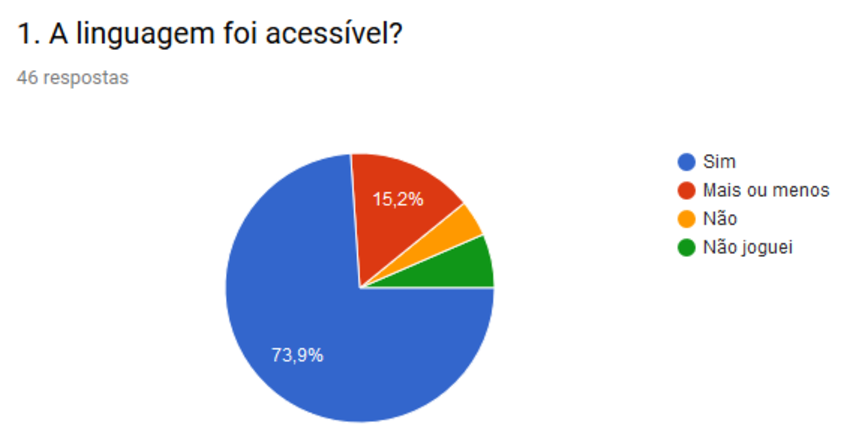
\includegraphics[width=0.9 \textwidth]{Resultados_e_Discussoes/Img_pesq_fin/resp_pesq_fin_02}
	\caption{Resultado da Pesquisa Final - Pergunta 1}
	\label{appb_fig:pf_res_perg1}
\end{grafico}

\begin{grafico}[ht]
	\centering
	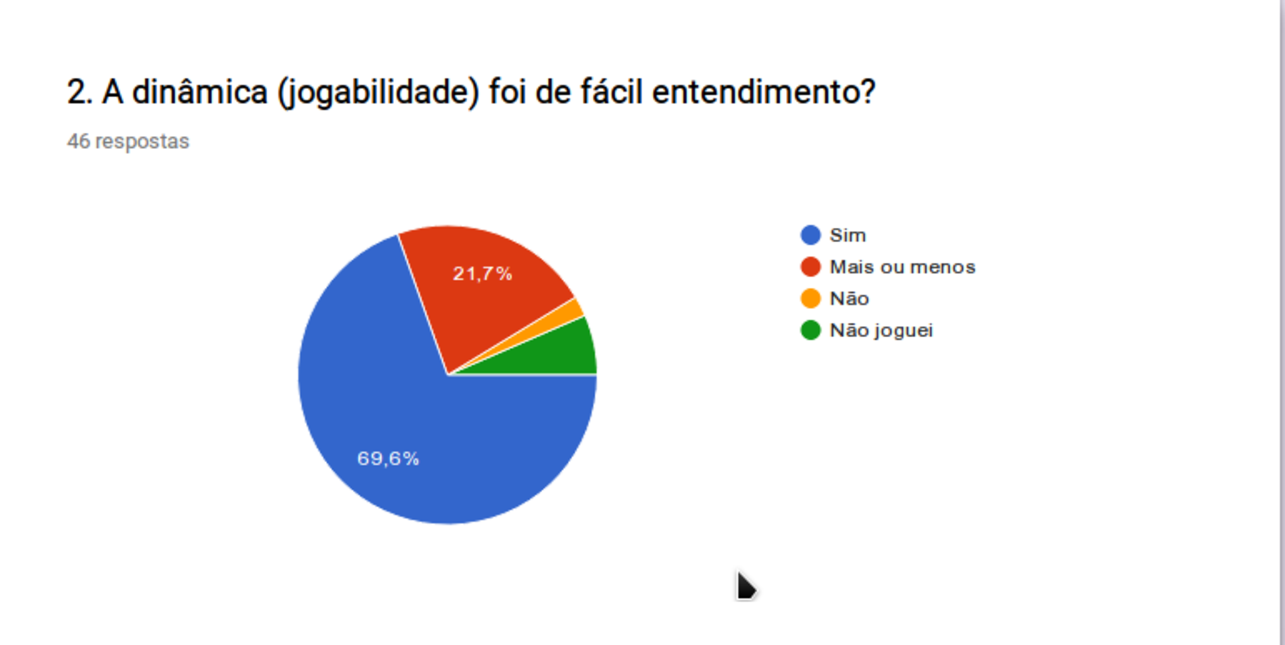
\includegraphics[width=0.9 \textwidth]{Resultados_e_Discussoes/Img_pesq_fin/resp_pesq_fin_03}
	\caption{Resultado da Pesquisa Final - Pergunta 2}
	\label{appb_fig:pf_res_perg2}
\end{grafico}

\newpage 

\begin{grafico}[ht]
	\centering
	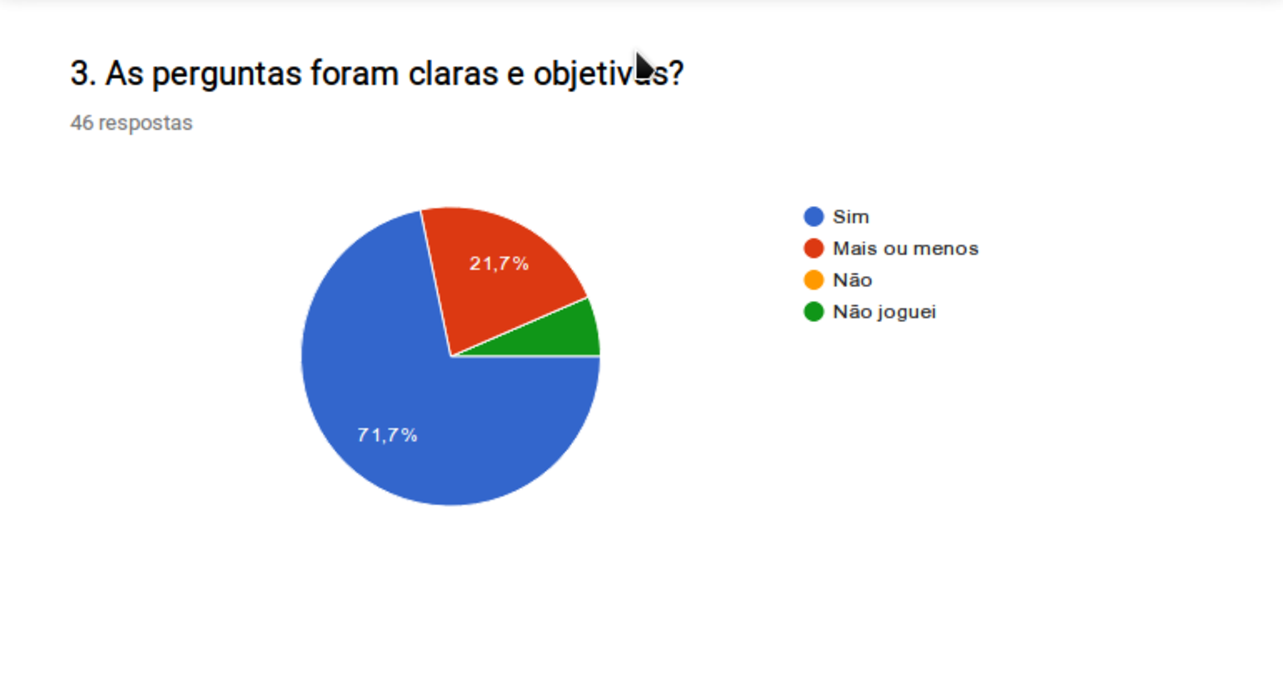
\includegraphics[width=0.9 \textwidth]{Resultados_e_Discussoes/Img_pesq_fin/resp_pesq_fin_04}
	\caption{Resultado da Pesquisa Final - Pergunta 3}
	\label{appb_fig:pf_res_perg3}
\end{grafico}

\begin{grafico}[ht]
	\centering
	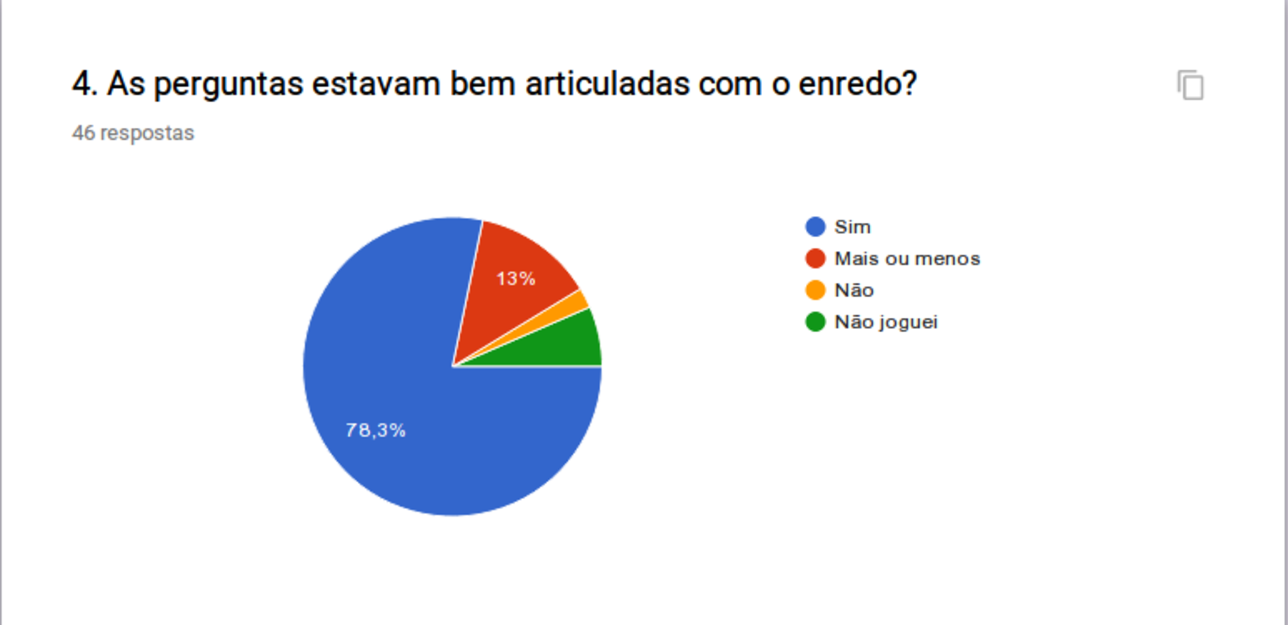
\includegraphics[width=0.9 \textwidth]{Resultados_e_Discussoes/Img_pesq_fin/resp_pesq_fin_05}
	\caption{Resultado da Pesquisa Final - Pergunta 4}
	\label{appb_fig:pf_res_perg4}
\end{grafico}

\newpage 

\begin{grafico}[ht]
	\centering
	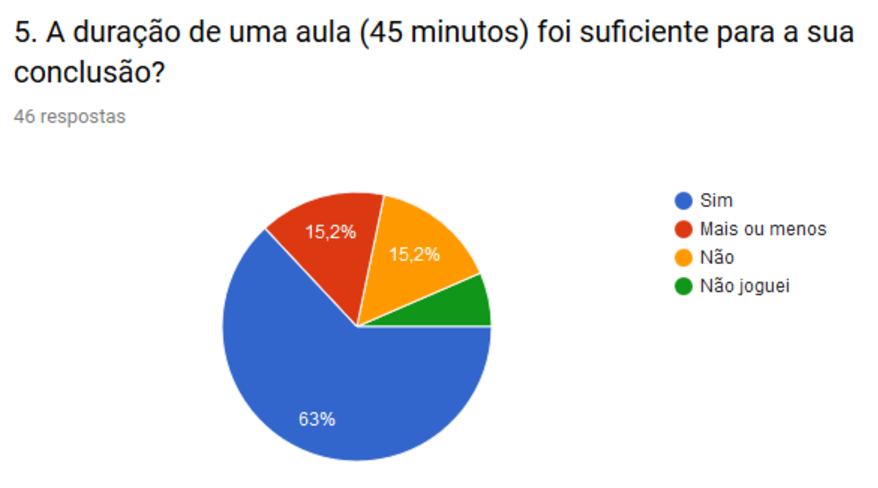
\includegraphics[width=0.9 \textwidth]{Resultados_e_Discussoes/Img_pesq_fin/resp_pesq_fin_06}
	\caption{Resultado da Pesquisa Final - Pergunta 5}
	\label{appb_fig:pf_res_perg5}
\end{grafico}

\begin{grafico}[ht]
	\centering
	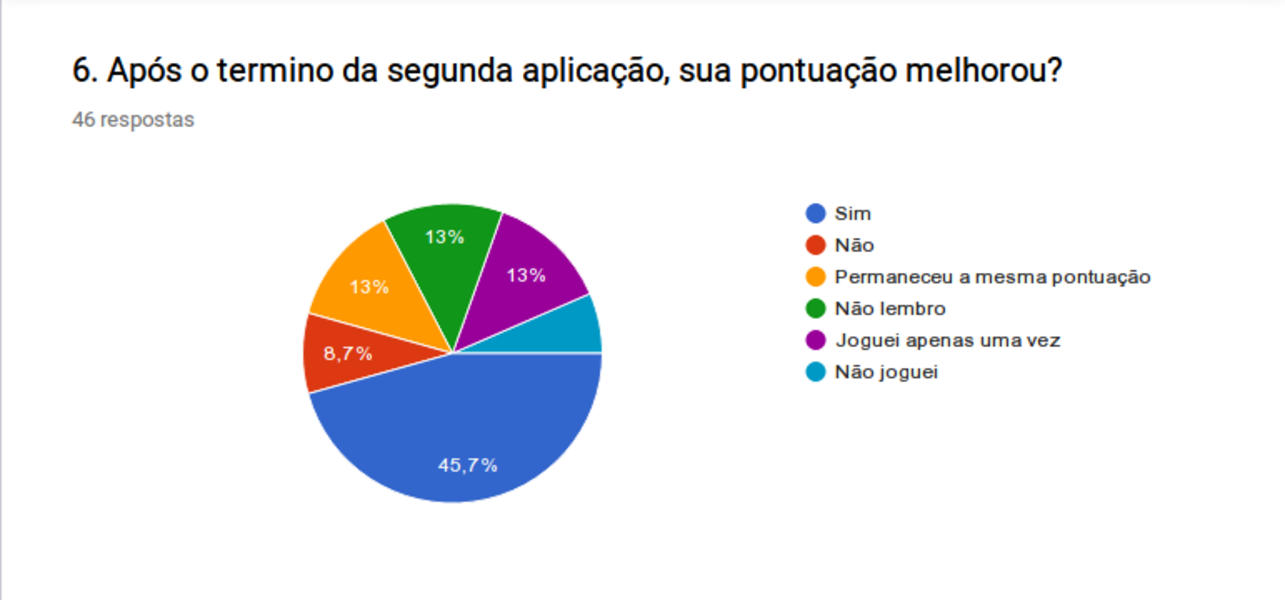
\includegraphics[width=0.9 \textwidth]{Resultados_e_Discussoes/Img_pesq_fin/resp_pesq_fin_07}
	\caption{Resultado da Pesquisa Final - Pergunta 6}
	\label{appb_fig:pf_res_perg6}
\end{grafico}

\newpage

\begin{grafico}[ht]
	\centering
	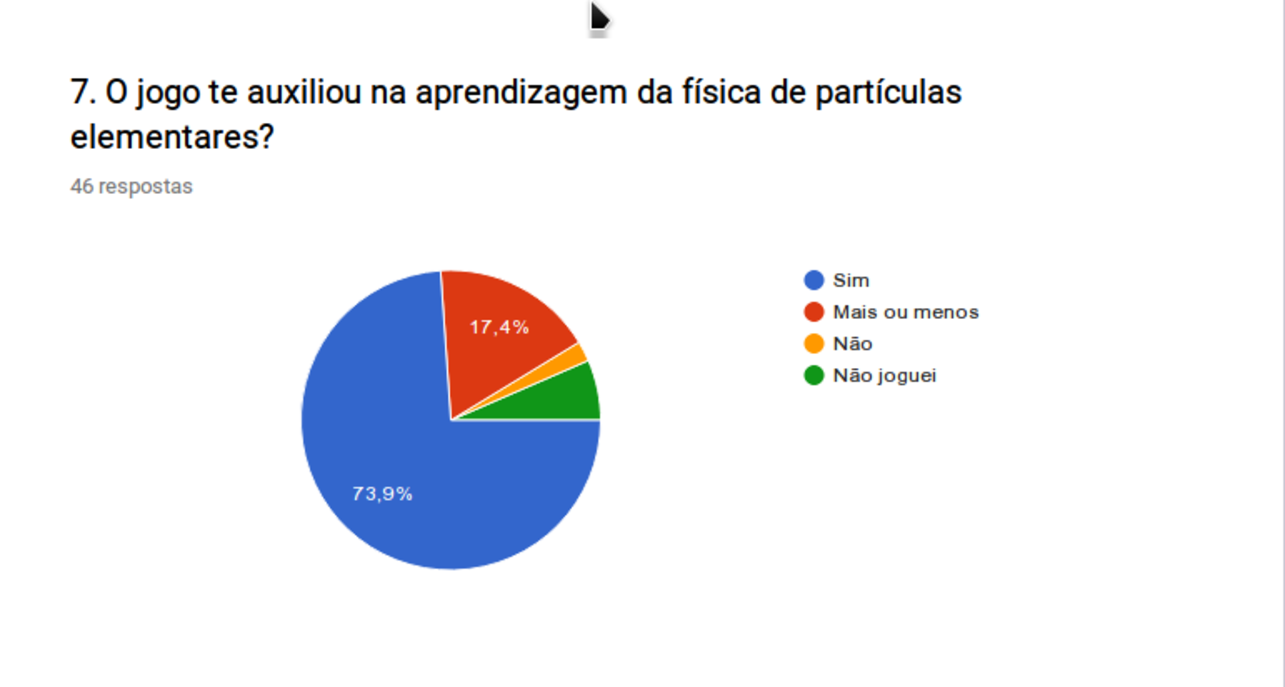
\includegraphics[width=0.9 \textwidth]{Resultados_e_Discussoes/Img_pesq_fin/resp_pesq_fin_08}
	\caption{Resultado da Pesquisa Final - Pergunta 7}
	\label{appb_fig:pf_res_perg7}
\end{grafico}

\begin{grafico}[ht]
	\centering
	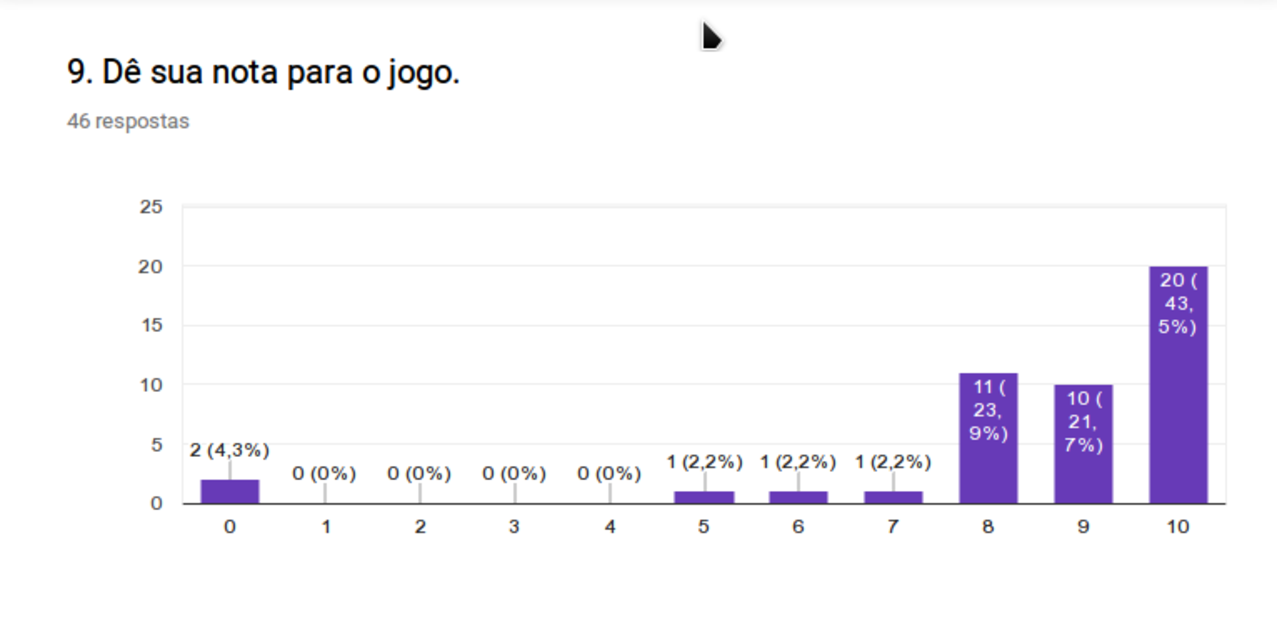
\includegraphics[width=0.9 \textwidth]{Resultados_e_Discussoes/Img_pesq_fin/resp_pesq_fin_15}
	\caption{Resultado da Pesquisa Final - Pergunta 9}
	\label{appb_fig:pf_res_perg9}
\end{grafico}

\newpage 

\begin{grafico}[ht]
	\centering
	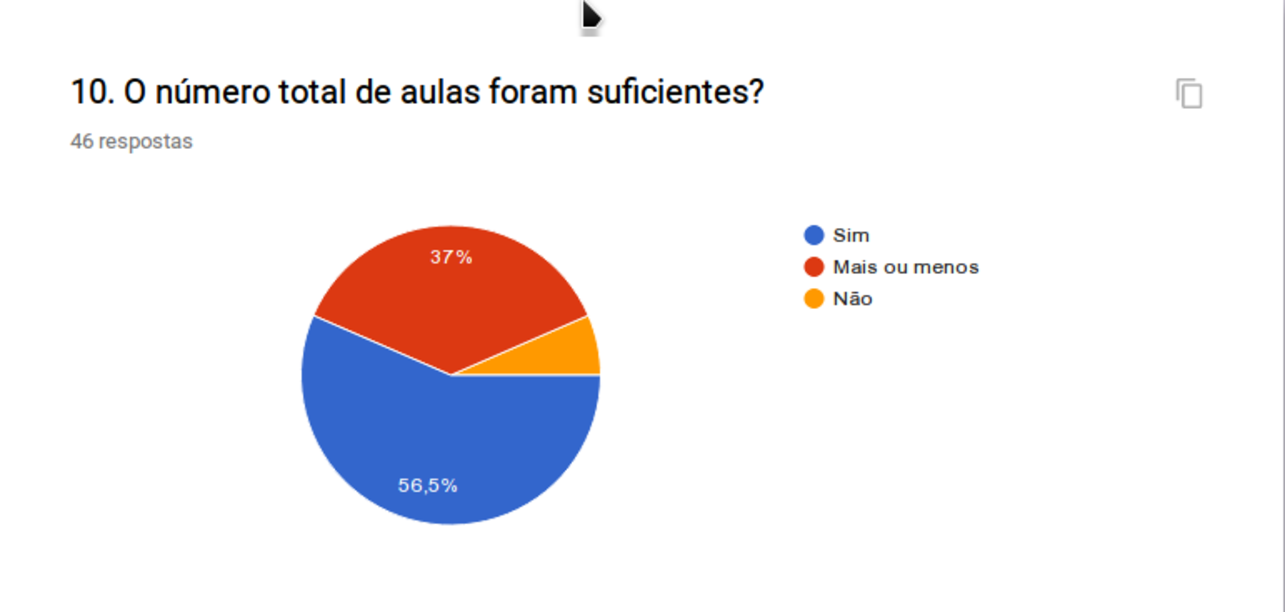
\includegraphics[width=0.9 \textwidth]{Resultados_e_Discussoes/Img_pesq_fin/resp_pesq_fin_16}
	\caption{Resultado da Pesquisa Final - Pergunta 10}
	\label{appb_fig:pf_res_perg10}
\end{grafico}

\begin{grafico}[ht]
	\centering
	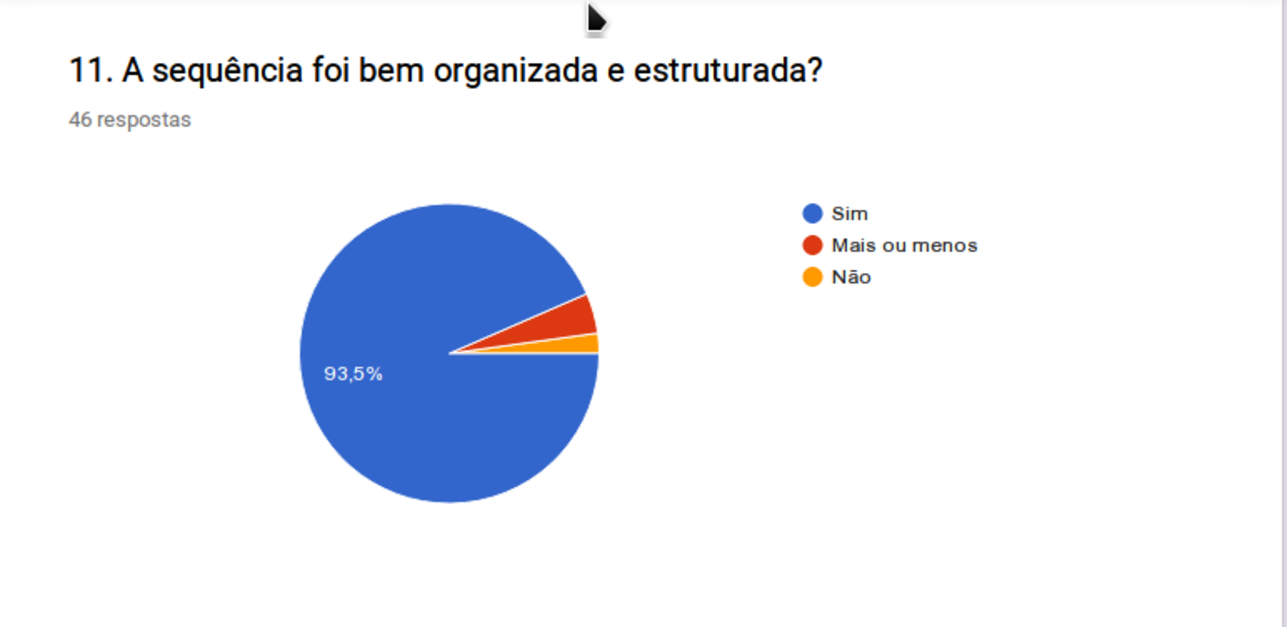
\includegraphics[width=0.9 \textwidth]{Resultados_e_Discussoes/Img_pesq_fin/resp_pesq_fin_17}
	\caption{Resultado da Pesquisa Final - Pergunta 11}
	\label{appb_fig:pf_res_perg11}
\end{grafico}

\newpage

\begin{grafico}[ht]
	\centering
	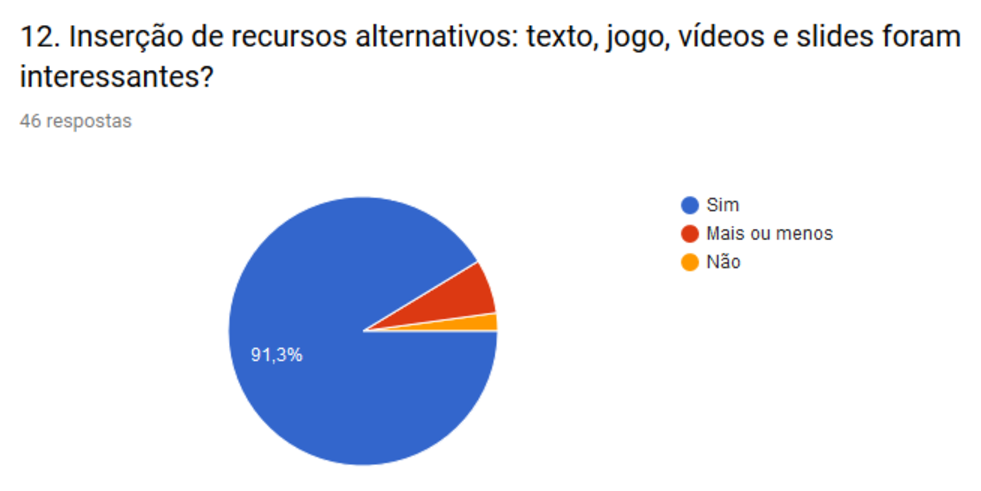
\includegraphics[width=0.9 \textwidth]{Resultados_e_Discussoes/Img_pesq_fin/resp_pesq_fin_18}
	\caption{Resultado da Pesquisa Final - Pergunta 12}
	\label{appb_fig:pf_res_perg12}
\end{grafico}

\begin{grafico}[ht]
	\centering
	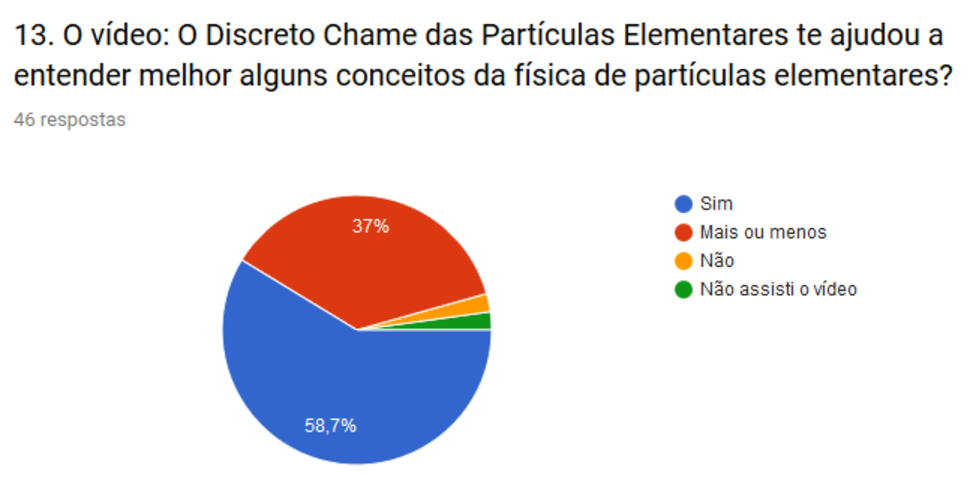
\includegraphics[width=0.8 \textwidth]{Resultados_e_Discussoes/Img_pesq_fin/resp_pesq_fin_19}
	\caption{Resultado da Pesquisa Final - Pergunta 13}
	\label{appb_fig:pf_res_perg13}
\end{grafico}

\newpage

\begin{grafico}[ht]
	\centering
	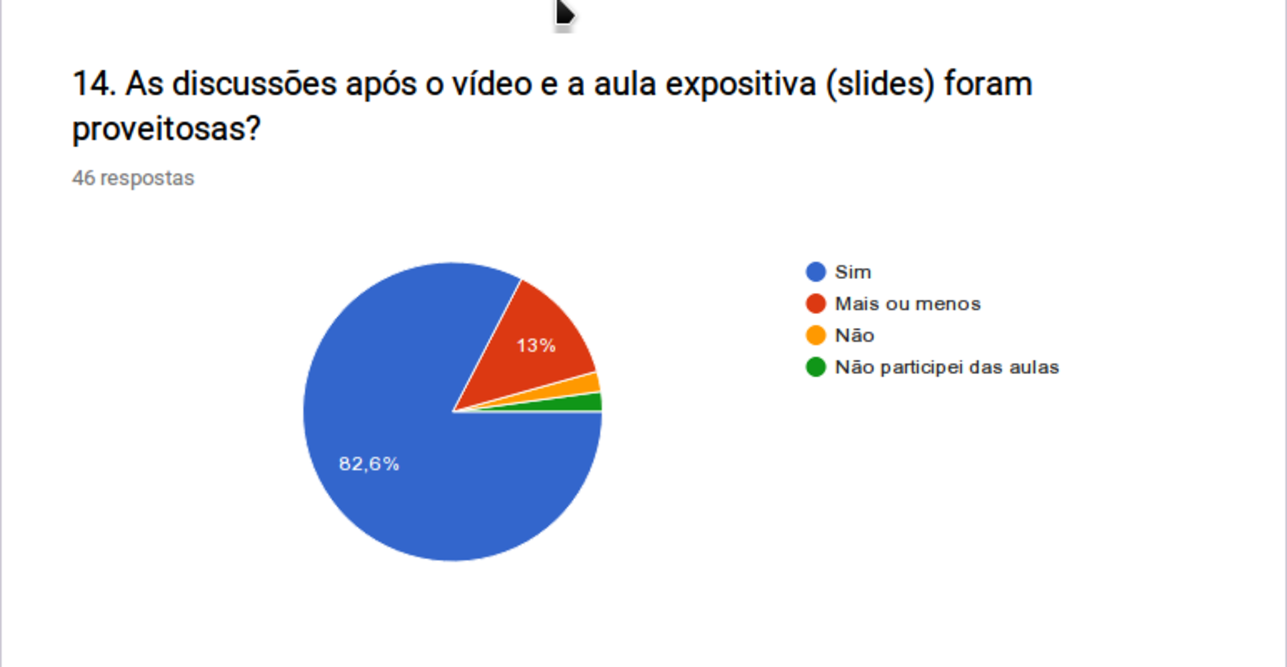
\includegraphics[width=0.8 \textwidth]{Resultados_e_Discussoes/Img_pesq_fin/resp_pesq_fin_20}
	\caption{Resultado da Pesquisa Final - Pergunta 14}
	\label{appb_fig:pf_res_perg14}
\end{grafico}

\begin{grafico}[ht]
	\centering
	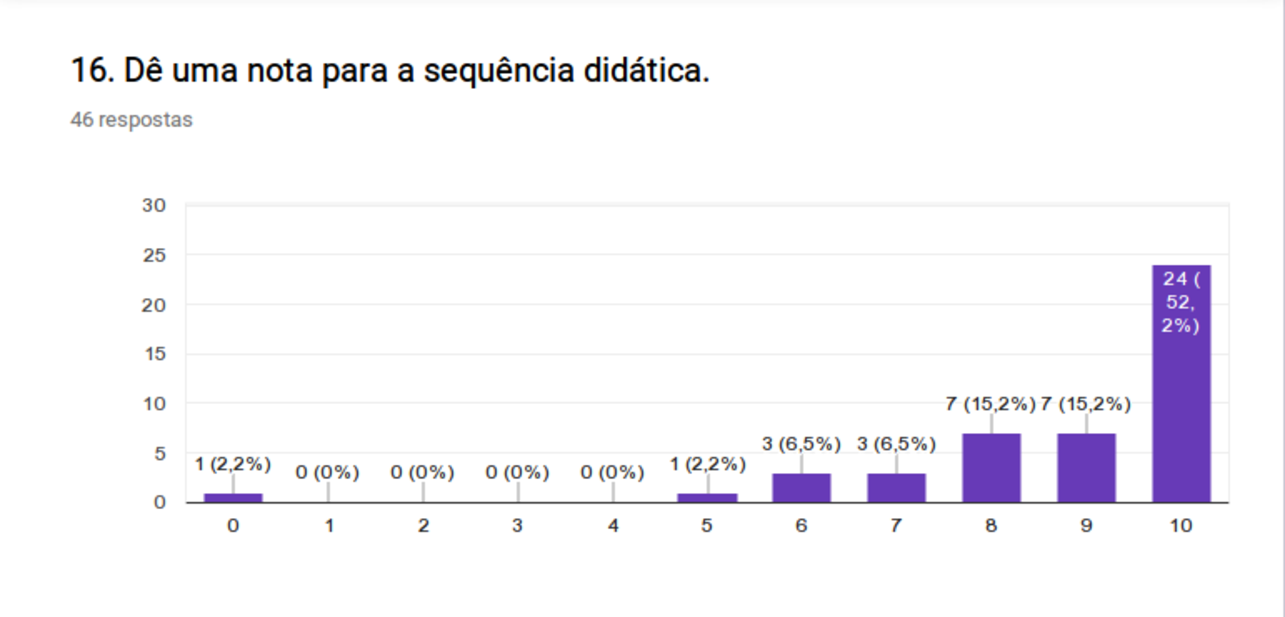
\includegraphics[width=0.8 \textwidth]{Resultados_e_Discussoes/Img_pesq_fin/resp_pesq_fin_25}
	\caption{Resultado da Pesquisa Final - Pergunta 16}
	\label{appb_fig:pf_res_perg16}
\end{grafico}

%\begin{figure}[h]
%\centering
%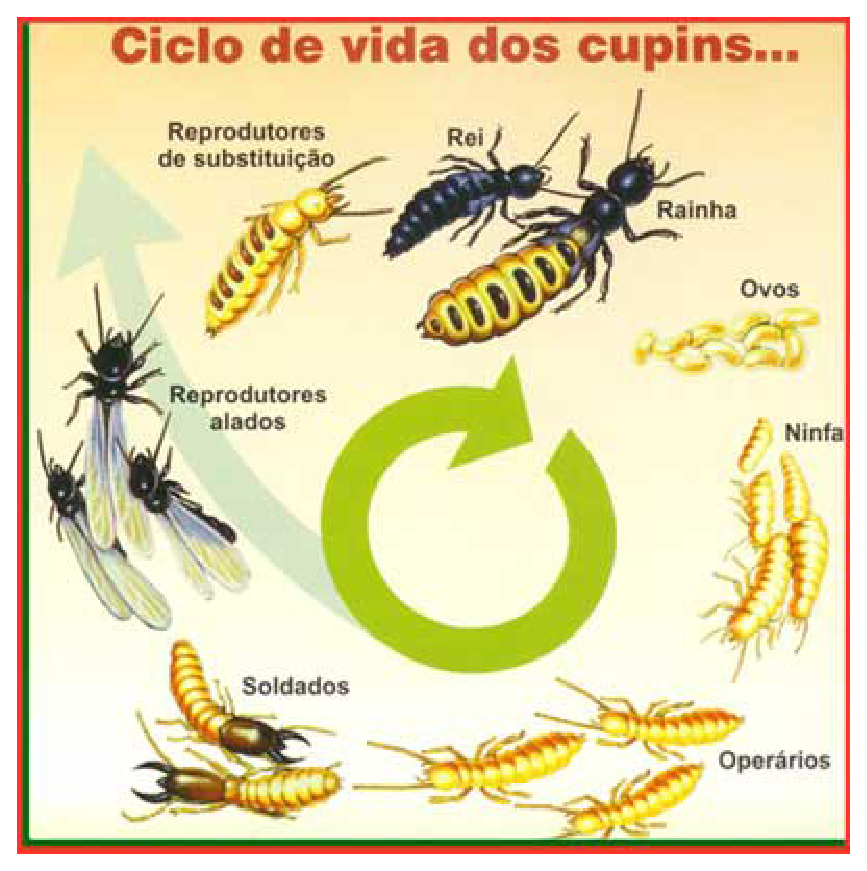
\includegraphics[height=5cm, width=5cm]{ApeA/pragas_ciclo_cupim}
%\caption{Uma figura que est� no ap�ndice}\label{FD}
%\end{figure}
